% CUSTOM_MAIN_TEX - do not overwrite (see report_builder.py preserve_existing_tex)
\documentclass[11pt,a4paper]{article}

\usepackage[a4paper,top=1.1in,bottom=1.1in,left=1.15in,right=1.15in]{geometry}
\usepackage[T1]{fontenc}
\usepackage{lmodern}
\usepackage{microtype}
\usepackage{ragged2e}
\usepackage{setspace}
\setstretch{1.15}
\usepackage{amsmath}
\usepackage{amssymb}
\usepackage{booktabs}
\usepackage{threeparttable}
\usepackage{longtable}
\usepackage{tabularx}
\usepackage{array}
\usepackage{enumitem}
\usepackage{caption}
\usepackage{float}
\usepackage{graphicx}
\usepackage{xcolor}
\usepackage{tikz}
\usepackage[round,authoryear,sort&compress]{natbib}
\usepackage{xurl}
\usepackage[colorlinks=true,linkcolor=black,citecolor=black,urlcolor=blue]{hyperref}
\usepackage{pdfpages}
\usepackage{fancyhdr}
\usepackage{titlesec}

\pagestyle{fancy}
\fancyhf{}
\fancyhead[L]{\small Simulation of Cyber-manipulation Susceptibility}
\fancyhead[R]{\small Ghent University}
\fancyfoot[C]{\thepage}
\setlength{\headheight}{14pt}
\setlength{\emergencystretch}{3em}

\setcounter{secnumdepth}{3}
\titleformat{\section}{\normalfont\large\bfseries}{\thesection}{0.6em}{}
\titleformat{\subsection}{\normalfont\normalsize\bfseries}{\thesubsection}{0.6em}{}
\titleformat{\subsubsection}{\normalfont\normalsize\itshape}{\thesubsubsection}{0.6em}{}
\titlespacing{\section}{0pt}{18pt}{6pt}
\titlespacing{\subsection}{0pt}{10pt}{4pt}
\titlespacing{\subsubsection}{0pt}{8pt}{3pt}

% APA-7 style: bold "Figure N." / "Table N." label, title on the next line in italics.
\DeclareCaptionLabelFormat{apa7}{\textbf{#1~#2.}}
\captionsetup{labelformat=apa7,labelsep=newline,textfont=it,justification=RaggedRight,%
  singlelinecheck=false,font=small,skip=3pt}

% Left-aligned floats (figures and tables are flush left, not centred).
\newcommand{\floatleft}{\setlength{\parindent}{0pt}\RaggedRight}
% APA-7 note placed underneath a figure or table.
\newcommand{\apanote}[1]{\par\vspace{3pt}\begingroup\footnotesize\setstretch{1.06}%
  \textit{Note.} #1\par\endgroup}
\newcommand{\suppheading}[1]{\par\vspace{10pt}\noindent{\small\bfseries #1\par}\vspace{3pt}}

\newcolumntype{Y}{>{\RaggedRight\arraybackslash}X}
\newcommand{\doiurl}[1]{\href{https://doi.org/#1}{https://doi.org/#1}}
\newcommand{\coverlinkoverlays}{%
  \begin{tikzpicture}[remember picture,overlay]
    \node[anchor=south west,inner sep=0pt] at ([xshift=143pt,yshift=278pt]current page.south west)
      {\href{https://github.com/stvsever/research_paper_on_cybermanipulation_susceptibility/tree/main}{\XeTeXLinkBox{\phantom{\rule{34pt}{13pt}}}}};
    \node[anchor=south west,inner sep=0pt] at ([xshift=143pt,yshift=260pt]current page.south west)
      {\href{https://github.com/stvsever/research_paper_on_cybermanipulation_susceptibility/tree/main/evaluation}{\XeTeXLinkBox{\phantom{\rule{34pt}{13pt}}}}};
  \end{tikzpicture}%
}

\begin{document}

\includepdf[pages=1,pagecommand={\thispagestyle{empty}\coverlinkoverlays}]{../assets/figures/cover.pdf}
\setcounter{page}{1}

\vspace*{1.9cm}
\begin{center}
\makebox[\linewidth][c]{%
\begin{minipage}{1.18\linewidth}
\centering
{\fontsize{26}{31}\bfseries\selectfont
Inter-individual Differences in Susceptibility to Cyber-manipulation of Political Opinions: An Ontology-based Multi-agent Simulation Approach\par}
\end{minipage}}
\vspace{1.2em}

{\normalsize
Stijn Van Severen$^{1}$ \quad Thomas De Schryver$^{1}$ \quad Mira Ostyn$^{1}$\par}
\vspace{0.4em}
{\small $^{1}$ Department of Experimental Psychology, Ghent University, Ghent, Belgium\par}
\end{center}

\vspace{1.0em}

\begin{abstract}
\noindent
Cyber-attacks increasingly target human cognition in addition to conventional
cybersecurity assets, yet investigating who is more susceptible by deliberately
manipulating citizens' opinions remains ethically untenable. Therefore, an ontology-based
multi-agent simulation pipeline is developed to audit adversarial influence in silico.
Three formal state spaces are constructed and crossed to sample scenarios from
(1)~high-resolution synthetic profiles, (2)~DISARM-based influence vectors represented as
ordered Plan, Prepare, and Execute operations, and (3)~opinion targets carrying an
adversarial direction. Across a maximum-entropy sample of 10,000 scenarios scored by
DeepSeek V4 Flash, simulated attacks shifted opinions toward the adversarial goal in 89\%
of scenarios (median $+14.4$ on a 2,001-position scale, Cohen's $d_z = 1.23$). The opinion
targeted dominated the outcome: issue domains differed markedly in manipulability
(Kruskal-Wallis $H = 579$, $p < .001$, $\varepsilon^2 = 0.067$), with infrastructure and
supranational-integration positions the most movable, with the political issue domains
explaining roughly thirty times more between-scenario variance than the entire 159-feature
profile battery. Susceptibility was nonetheless strongly heterogeneous across individuals
while only weakly aligned with measured traits: openness and neuroticism predicted greater
movement ($\beta = +0.042$, $q = .004$; $\beta = +0.030$, $q = .040$), conscientiousness
predicted resistance ($\beta = -0.035$, $q = .012$), and the political-attitude batteries
contributed little (cross-validated $R^2 \approx 0$). Because the estimates are produced in
silico, they are interpreted as directional hypotheses for subsequent human validation.
\end{abstract}

\vspace{0.6em}

\clearpage
\section{Introduction}

\subsection{Cyber-manipulation as a Cognitive-security Problem}

Cyberattacks have grown into a pervasive and escalating threat, increasing in both
volume and sophistication \citep{councileu2025cyber,liliu2021comprehensive}. Their harm
is multidimensional: economic, through value extraction and loss; operational, because
the most prominent threats target the availability of systems and data; and social and
psychological, as victims report anxiety, trauma, and helplessness
\citep{bada2020social,councileu2025cyber}. It also cuts across every level of
organisation, reaching the individual whose wellbeing and data are targeted, the
company whose viability a disruption can threaten, and the nation and supranational body,
for which attacks on critical infrastructure are a strategic concern
\citep{bada2020social,ryan2025impact}.

Within this landscape, the frontline has shifted from breaching systems to exploiting
people directly. Identity-centric intrusions and social engineering, increasingly
powered by AI-generated deepfakes and phishing, now dominate the threat picture
\citep{bada2020social,inkster2023cybersecurity,mcconkey2026annual}. The same
human-centric techniques are turned on political opinion. The European Union treats
foreign information manipulation and interference (FIMI), in which cyber capabilities
and coordinated influence operations converge to shape public discourse and steer
attitudes on questions such as alliances and foreign powers, as a core threat, amplified
by AI-generated content and aimed at elections, journalists, and public sentiment
\citep{enisa2023elections,enisaeeas2022fimi}. This unfolds as political attitudes harden.
Affective polarisation has risen across many democracies \citep{reiljan2020fear}, and a
polarised public is not uniformly more persuadable but rather more entrenched against
opposing messages while more open to influence that confirms its existing identity and
commitments. Understanding who can be moved, on which issues, and by which technique
therefore becomes a question of democratic resilience rather than individual security
alone. Cyber-defence on this surface is a cognitive-security problem: the asset under
attack is the citizen's capacity to form and revise political beliefs autonomously.

\subsection{Formalizing Cyber-manipulation Attacks in the Information Environment}

The covert movement of political opinion is treated here as adversarial influence rather
than ordinary persuasion. Following \citet{susser2019technology}, manipulation is the
covert exercise of influence: intentionally steering another person's choices by
targeting and exploiting their decision-making vulnerabilities, in a way the target is
neither aware of nor could easily become aware of. Covertness is what separates it from
persuasion, which is forthright, offering reasons the target can consciously weigh and
accept or reject, so that deliberation stays intact and the influence is recognised for
what it is \citep{botes2023autonomy,sheikh2023persuasion}. Deception and coercion sit on
the same side as manipulation: deception plants false beliefs, and coercion narrows a
person's options until the intended choice becomes the only rational one
\citep{botes2023autonomy}. What unites these three and divides them from persuasion is
that each bypasses or overrides autonomous deliberation rather than engaging it, which is
why each constitutes a harm to autonomy rather than a legitimate appeal to it
\citep{botes2023autonomy,susser2019technology}. Applied to political opinion this harm is
also collective, because democratic self-governance presupposes citizens who form and
revise their views autonomously \citep{susser2019technology}.

If manipulation is the harm, a structured account of how it is carried out is needed
before asking who is vulnerable to it. That account is drawn from DISARM, an openly
maintained, standardised taxonomy of disinformation tactics derived from cybersecurity
practice and endorsed by ENISA and the EEAS \citep{disarmfoundationnd,enisaeeas2022fimi}.
DISARM transposes the intrusion kill chain, the staged decomposition of an adversary
campaign from planning through preparation to objective \citep{hutchins2011intelligence},
from network defence to the information environment. It decomposes an influence operation
into ordered phases and the concrete, reusable techniques that realise them, which turns
an open-ended notion of an attack into a finite and comparable set of interventions that
can be instantiated as artifacts and crossed against individual profiles. Each DISARM
technique is accordingly treated as a candidate attack whose effect on political opinion
is the quantity of interest.

\subsection{Predictive Characteristics of Cyber-manipulation Susceptibility}

Susceptibility to such influence is theorised to be patterned by stable individual
differences, and the dimension most often invoked is personality as organised by the
five-factor model: openness, conscientiousness, extraversion, agreeableness, and
neuroticism. Two recent systematic reviews bracket the phenomenon from a legitimate and an
adversarial end. Reviewing persuasion strategies, \citet{palmtims2025influence} report that
responsiveness is graded by trait, with agreeableness the most susceptible and neuroticism
the least, and that appeals matched to a recipient's dominant trait outperform generic ones
whereas mismatched appeals can be actively counterproductive. Reviewing phishing,
\citet{lopezaguilar2025phishing} find that extraversion, agreeableness, and neuroticism are
generally associated with greater vulnerability, that conscientiousness emerges as
protective, and that openness remains inconclusive. Considered jointly, the two reviews converge
on agreeableness as susceptible and conscientiousness as resistant, and diverge on
neuroticism, which would be least susceptible to ordinary persuasion yet among the more
vulnerable to phishing. The tension eases once the content of the appeal is considered,
since neurotic individuals resist generic persuasion but respond to threat, urgency, and
scarcity \citep{lopezaguilar2025phishing,palmtims2025influence}.

Overall susceptibility is therefore a coarse summary, as traits respond selectively to
particular influence principles rather than to influence as such
\citep{palmtims2025influence}. The evidence is also largely correlational and drawn mostly
from consumer, health, and security settings rather than political opinion. In the political
domain itself, \citet{decker2023personality} found no extraversion effect on microtargeted
persuasion and argued that a single trait is too thin a basis for targeting in a domain as
complex as democratic discourse. Personality thus plausibly conditions who is moved, but
contingently on which technique meets which trait and on which opinion is targeted.

\subsection{Ethical Limitations of Research on Cyber-manipulation}

Studying this mechanism directly in human populations is sharply constrained. The strongest
designs are also the least transferable to adversarial cyber-attack research. The Cambridge
Analytica episode of 2016 made the ambition concrete and public: the firm claimed to fuse
social-media traces with psychometric profiles in order to link information vectors to
individual susceptibility and to microtarget political advertising that would sway votes,
and the ensuing data scandal exposed both the commercial appetite for such methods and the
scale at which they could be attempted \citep{susser2019technology,isaak2018user}. Its
actual electoral impact, however, was never demonstrated and remains contested, because the
firm's effectiveness claims were promotional rather than evidential. Controlled evidence that
psychological targeting can shift behaviour at scale comes instead from randomized controlled
field experiments. Large platform experiments have moved real political behaviour at
population scale through social cues \citep{bond2012experiment} and have altered emotional
state through feed manipulation \citep{kramer2014experimental}, and personality-matched
advertising has raised engagement and conversion in live campaigns
\citep{matz2017psychological}, even as later estimates place the persuasive returns to
political microtargeting as real but modest \citep{tappin2023quantifying}.

These same experiments mark the ethical boundary of the field. The designs that would most
cleanly estimate susceptibility, randomly exposing citizens to covert manipulation,
systematically varying hostile tactics, and optimising persuasion against vulnerable
subgroups, are precisely the designs that cannot be run on real people without violating
consent and autonomy \citep{kramer2014experimental,susser2019technology}. Deliberately
manipulating citizens' political opinions to learn who is most movable is ethically
untenable, and even a fully consented study could not map the combinatorial space of who is
moved by which technique on which issue without an impractically large factorial. The
mechanism therefore remains under-measured exactly where it matters most, which motivates an
approach that can explore the adversarial state space before any human is exposed.

\subsection{Semantic Technologies for In-silico Susceptibility Auditing}

Generative artificial intelligence has made this form of influence cheap, fast, and
scalable. Messages written by openly available large language models (LLMs) shift policy
attitudes in the advocated direction, with effects that are small but comparable to those of
lay human authors and largely indistinguishable from human-authored text to readers
\citep{bai2025llm}. The more acute concern is not generic AI text but tailoring: pairing
automated generation with psychological profiles inferred from digital traces yields a
pipeline that can microtarget at population scale with little human input
\citep{matz2024potential,simchon2024persuasive}. Appeals matched to a recipient's
personality, ideology, or moral foundations tend to be rated more persuasive than
non-personalised ones and accumulate into consequential aggregate effects once distributed
across many recipients \citep{matz2024potential,simchon2024persuasive}.

The same semantic technologies that scale the threat also make it auditable. LLMs conditioned
on demographic and attitudinal backstories can serve as proxies for human subpopulations,
reproducing population-level patterns of opinion with what \citet{argyle2023out} term
algorithmic fidelity. Together with a longer tradition of agent-based modelling of
heterogeneous social actors \citep{macy2002factors,cioffirevilla2002invariance} and of LLM
agents that reason over rich social contexts \citep{park2023generative}, this makes it
possible to instantiate a population of synthetic personas, expose each to a manipulative
artifact, and measure the resulting shift in opinion before any human is exposed. Ontology-based
state-space modelling supplies the missing structure for such an audit. Rather than improvising
prompts, the simulated person, the adversarial operation, and the opinion target are each
represented as an explicit hierarchical ontology that fixes the admissible universe of values
before any model call is made. A profile encodes an individual's attributes (demographics,
socioeconomics, the five-factor model, a political-psychology battery, moral foundations,
religion, and digital literacy); an attack encodes a manipulative intervention drawn from
DISARM and instantiated as a realistic operation; and an opinion encodes a target belief
dimension carrying an adversarial direction, so that any movement can be scored as success or
resistance. Crossing these components yields scenarios in which an agent reports a baseline
opinion, is exposed to the attack, and reports its opinion again; the signed, direction-aware
change is the attack's effectivity, positive when the agent moves toward the attacker's goal
and negative when it resists or backfires.

\subsection{The Present Study}

Opinion change is not only an individual event but a socially embedded one. People are also
moved by exposure to the views of those around them, and a surrounding network can reinforce
or counteract a given message \citep{bail2018exposure}. The framework therefore comprises two
layers: an individual layer, in which susceptibility is measured for a person scored in
isolation, and an exposure-network layer built on an empirical social-media network, in which
opinions formed in isolation are compared with opinions formed under network exposure. These
strands are rarely examined jointly; prior work tends to isolate one factor while holding the
others fixed, leaving the interaction of technique, profile, opinion, and network largely
open.

The present framework is designed as a hypothesis-generating instrument for investigating the
high-resolution dynamics of influence vectors across the joint space of profiles, attacks, and
opinions. Because the tests are conducted in silico, the resulting estimates are read as
predictions to be validated in human populations rather than as established human effects. Two
research questions organise the work, one on the individual layer and one on the network layer:

\begin{enumerate}[label=\textbf{RQ\arabic*.},leftmargin=3.4em,itemsep=3pt]
\item To what extent, and in which direction, do DISARM-based attacks shift political
opinions, and which profile characteristics moderate this directional effectivity,
conditional on the attack used and the opinion targeted?
\item How do private susceptibility differences translate into network-conditioned
cyber-manipulation effects, and does population-level amplification depend on whether
susceptible or resilient profiles occupy high-reach positions in an empirical exposure network?
\end{enumerate}

\noindent The methodology and results first develop the individual layer and then extend the
same profile, attack, and opinion framework into the empirical exposure-network layer. The
directional hypotheses associated with both research questions are stated, with the design, in
Section~\ref{sec:hypotheses}.

\section{Method}

\subsection{Simulation Design Overview}

The study uses an ontology-based simulation design in which each observation is a structured
scenario linking one synthetic profile, one DISARM-red influence operation, and one opinion
issue-domain cluster. Figure~\ref{fig:pipeline} gives the architecture end to end: three
independent ontological state spaces are defined, a maximum-entropy sampler crosses them into
scenarios, schema-constrained LLM agents return a private baseline and a post-attack opinion
for every opinion leaf, a direction-aware effect is constructed per leaf, and the inferential
layer estimates attack effectiveness, opinion and attack-factor effects, profile moderation,
and reliability.

Each opinion cluster contains multiple directional opinion leaves, which are scored in a single
cluster-batched measurement and then expanded to per-leaf records for analysis. The design is
attacked-only, because the estimand is not the average effect of attack presence versus absence
but direction-aware susceptibility conditional on a specified profile, operation, and opinion
target. For a profile $i$ and opinion leaf $\ell$ with adversarial direction
$d_\ell \in \{-1,+1\}$, the private baseline opinion $B_{i\ell}$ and post-attack opinion
$P_{i\ell}$ define adversarial effectivity
$\mathrm{AE}_{i\ell} = (P_{i\ell}-B_{i\ell})\,d_\ell$, the signed distance moved toward the
attacker's goal. This individual effect is $\Delta_{\text{direct}}$ in the terms of RQ1. The
unit of analysis is the scenario: the roughly fifteen opinion-leaf measurements within a
scenario are averaged before any profile-level model, so each scenario contributes one
independent value and clustered leaves are not treated as independent observations.

\begin{figure}[ht]
\floatleft
\caption{Ontology-based Simulation Pipeline with Network Exposure Layer}
\label{fig:pipeline}
\vspace{2pt}
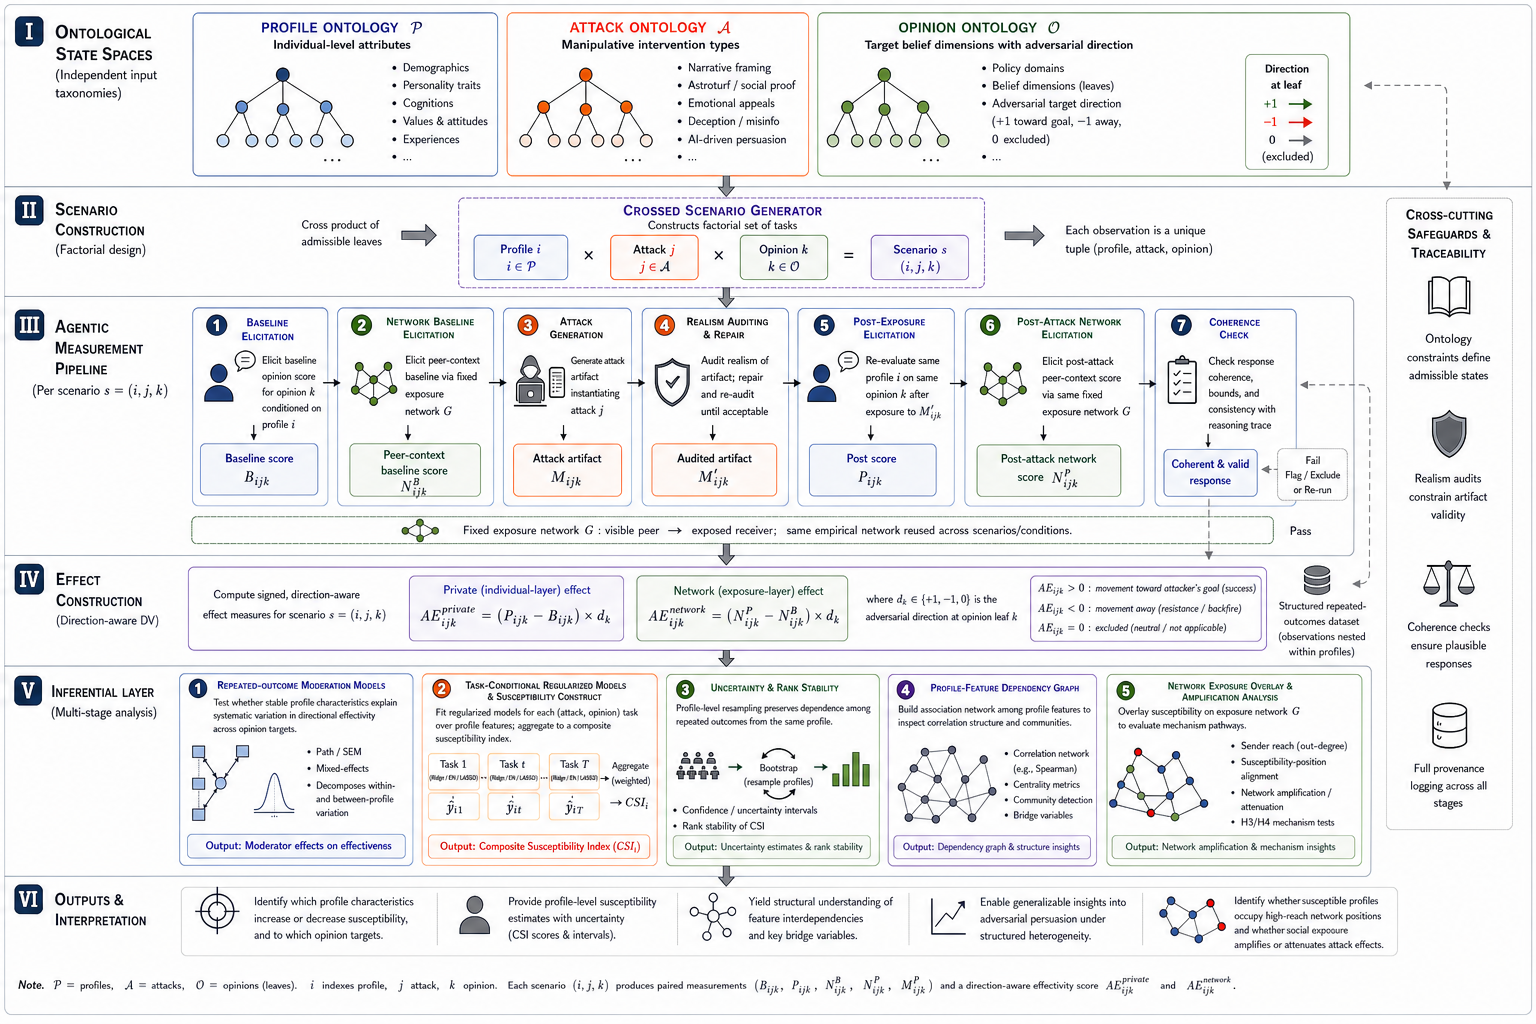
\includegraphics[width=\linewidth]{../assets/figures/main/MAIN1_pipeline_network_layer.png}
\apanote{From left to right: (I)~three ontological state spaces (profile, attack, opinion)
define the admissible universe; (II)~a maximum-entropy sampler crosses one profile, one
DISARM-red triplet, and one opinion leaf into each scenario; (III)~schema-constrained
agents elicit private baseline opinions $B$, baseline opinions after exposure to the empirical
peer network $N^B$, private post-attack opinions $P$, and post-attack opinions after the same
network exposure $N^P$; (IV)~direction-aware private and network effect measures are
constructed using the adversarial direction $d$; (V)~the inferential layer estimates
individual susceptibility, task-conditional effects, profile moderation, and network-exposure
mechanisms. The fixed exposure graph $G$ is reused across network-conditioned measurements,
with edges directed from visible peer to exposed receiver.}
\end{figure}

\subsection{Ontological State Spaces}

The pipeline begins from three independent state spaces: profile, attack, and opinion. These
are not loose prompt templates but formal ontologies that define the admissible universe of
simulated persons, adversarial operations, and measurable opinion targets before any model
call is made. This matters because the central threat to inference in a simulation of this kind
is range restriction: if profiles are sampled from a narrow demographic frame, attacks from a
small set of familiar manipulations, or opinions from a few salient policy items, any estimated
susceptibility pattern may reflect design convenience rather than the structure of the
phenomenon. Each ontology is represented as a recursively populated tree with stable paths.
Terminal leaves carry structural metadata (modality type, sampling role, exclusivity group,
prevalence weight, adversarial direction, and compatibility constraints), and higher-level rules
propagate metadata over whole subtrees. LLM assistance during ontology construction was limited
to candidate generation, naming, and wording under human curation; the executed simulation does
not allow a model to add, remove, or reweight ontology leaves, and the ontologies do not encode
downstream hypotheses such as a link between neuroticism and fear-appeal susceptibility. Those
relationships are estimated from the simulated outcomes, not assumed by the design.
Table~\ref{tab:spaces} summarises the three spaces and their production frames.

\subsubsection{Profile ontology}

The profile ontology represents a high-resolution synthetic person as a nested hierarchy of
individual-difference constructs rather than a flat list of variables. Its branches span
demographic position (age, sex, ethnocultural background, citizenship, migration history),
household and life-course context, education and work, socioeconomic position, geography and
urbanicity, religion and worldview, media habits and digital literacy, and a deep psychological
core. That core carries the five-factor model resolved to its facets, a political-psychology
battery (right-wing authoritarianism, social dominance orientation, system justification,
populist attitudes, collective narcissism, nationalism and cosmopolitanism, political trust and
legitimacy, political efficacy, and a dual-process motivational model), the two-axis ideological
space (economic left-right, socio-cultural liberal-conservative, the GAL-TAN dimension, and the
libertarian-authoritarian dimension), and moral-foundations theory (care, fairness, loyalty,
authority, and sanctity). This breadth is deliberate, because susceptibility is not expected to
reduce to a single variable family: a profile may resist a claim because of prior knowledge,
identity-consistent opposition, low trust in the implied source, or conflict with moral and
ideological commitments, and an ontology that omitted any of these channels would confound
absence of measurement with absence of effect.

The sampler reads the structural metadata attached to each leaf and assembles coherent
full-profile assignments. Categorical variables are drawn as mutually exclusive options subject
to coherence rules; continuous psychometric constructs are drawn as percentile-valued dimensions
or facets; ordinal variables preserve their order; and trait scalars such as age are drawn on
their native scale. Sampling follows a maximum-entropy principle balanced against realistic
prevalence, so the frame spans the admissible space broadly, and counteracts range restriction,
without collapsing into deterministic stereotypes or implausible attribute combinations.
Coherence rules are applied before a profile is released, which removes logically incompatible
assignments while leaving the joint distribution otherwise unconstrained. The Issue Position
Taxonomy is excluded from the profile space, because issue positions are the outcomes an
adversary attempts to move, not stable background features to be sampled as attributes. The full
production frame contains 272 categorical variables with 1,467 options, 41 continuous scale
groups with 181 scale leaves, 26 ordinal variables, 6 trait scalars, and 7 identifiers. For the
present run the profile was reduced to roughly 159 analysis features, retaining the full
hierarchical Big Five, the core demographic markers, and the political-psychology, ideology, and
moral-foundations batteries, while dropping the most granular socioeconomic, life-circumstance,
and identity spectra that are peripheral to RQ1; this reduction keeps the moderator space
interpretable while preserving the constructs theorised to predict susceptibility.

\subsubsection{Opinion ontology}

The opinion ontology represents the targets that an operation can move and is restricted, for
attack measurement, to the Issue Position Taxonomy. Issue-position leaves are concrete,
survey-like policy statements that can be scored on a bipolar opinion scale and assigned a
defensible adversarial direction, which makes them suitable outcomes; broader psychological
constructs are valuable for profile definition but lack a clear direction of adversarial
success and are therefore not scored as outcomes. The sampled frame contains 106 directional
issue-position leaves grouped into 7 issue-domain clusters: Critical Infrastructure and Energy
Sovereignty, Defense and National Security, Democratic Resilience and Institutions, Foreign
Policy and Geopolitics, Information Integrity and Platforms, Supranational and Regional
Integration, and Macroeconomic and Fiscal Policy. The clusters are substantively distinct
attack surfaces, ranging from technocratic-infrastructural positions (for example, nuclear-power
investment, energy-sovereignty investment, supply-chain resilience) through security and
geopolitical positions (common defense capacity, cyber-defense standards) to institutional and
informational positions (judicial independence, platform accountability, journalistic trust).

Each leaf carries an adversarial direction $d_\ell \in \{-1,+1\}$, encoding the goal an attacker
would pursue against that position: $+1$ where the goal is to amplify support and $-1$ where the
goal is to erode it. Direction-neutral leaves remain in the broader ontology for completeness
but are excluded from primary effectivity scoring, because a movement on a neutral item cannot
be scored as success or resistance. The direction is a property of the opinion target rather
than of any particular attack, which is what allows the signed effectivity to be compared across
heterogeneous operations. Clusters are measured as coherent issue domains so the agent reasons
with full topical context and adjacent positions are not stripped of their relationships, but
every inferential outcome is computed at the leaf level, because the same person can plausibly
support one position in a domain while opposing another, and averaging across opposing directions
within a domain would cancel genuine movement. The single-leaf Macroeconomic and Fiscal Policy
domain is retained in the ontology but excluded from every analysis and figure as a statistical
outlier, which leaves 6 analysed domains.

\subsubsection{Attack ontology: DISARM-red triplets}

The attack ontology is drawn from an external DISARM-red frame rather than a small bespoke
taxonomy, which reduces the risk that the study tests only familiar or easily imagined attacks
and makes the attack space analytically decomposable. DISARM is the openly maintained
counter-disinformation counterpart of the adversarial kill chain and of the technique
catalogues used in network defence: it organises an influence operation into ordered tactical
phases and, within each phase, a catalogue of concrete techniques and procedures
\citep{disarmfoundationnd,enisaeeas2022fimi,hutchins2011intelligence}. The Red frame describes
the attacker side of that model, so that an attack can be specified at the same level of
structure that defenders use to detect and categorise real operations.

Each attack is represented as a three-phase Plan, Prepare, and Execute triplet that mirrors the
staged logic of a campaign. The Plan phase fixes the strategic objective and audience logic
(for example, planning around objectives versus target-audience analysis); the Prepare phase
fixes the assets and enabling conditions (developing content or narratives, establishing assets
or legitimacy, microtargeting, or selecting channels and affordances); and the Execute phase
fixes the delivery or manipulation technique (for example, delivering content, conducting pump
priming, maximising exposure, driving online harms or offline activity, or persisting in the
information environment). This triplet structure is central to the design. Campaign-like attacks,
including astroturfing, multi-persona amplification, synthetic-content operations, and platform
gaming, cannot be reduced to a single message read once; the simulation therefore passes the
resolved triplet and its signal attributes to the agent as an operation specification, and the
agent estimates the profile's likely opinion state under that operation rather than rating the
literary quality of one generated text. Each configuration additionally carries a complexity
tier, from atomic single-technique operations (T1) through campaign (T2) and synthetic-media
(T3) to fully orchestrated multi-component operations (T4), which supports a dose-response test
of operational sophistication, together with a quantitative opinion-manipulation signal score
and an inclusion route that record how strongly and through which pathway a configuration is
expected to bear on opinion.

The source frame begins from 3,317 Plan, 8,059 Prepare, and 8,318 Execute leaves, a full
Cartesian upper bound of 222,354,305,554 possible triplets. A coherence-and-relevance filter
retains plausible opinion-manipulation configurations and removes support-only, logistics-only,
access-only, and operational-security-only combinations, yielding 48,991 filtered configurations
over 17,941 distinct leaves. This filtering keeps the attack space large enough to resist range
restriction while excluding combinations that could not realistically bear on a political
opinion. The full attack ontology is treated as dual-use material and is not reproduced here.

\begin{table}[htbp]
\floatleft
\caption{The Three Ontological State Spaces and Their Production Frames}
\label{tab:spaces}
\vspace{2pt}
\begingroup\small
\begin{tabularx}{\linewidth}{@{}p{0.13\linewidth}YYp{0.17\linewidth}@{}}
\toprule
State space & Hierarchical structure and metadata & Production-frame cardinality & Role in a
scenario \\
\midrule
Profile & Recursive tree of individual-difference constructs: demographics, life context,
five-factor facets, political psychology, ideology, moral foundations, socioeconomics,
information behaviour & 272 categorical variables / 1,467 options; 41 continuous groups / 181
scale leaves; 26 ordinal; 6 trait scalars; 7 identifiers ($\approx$159 features analysed) & The
simulated person whose attributes may moderate susceptibility \\[2pt]
Opinion & Issue Position Taxonomy of directional policy positions nested in issue-domain
clusters; each leaf carries $d_\ell \in \{-1,+1\}$ & 106 directional leaves in 7 clusters (6
analysed); neutral leaves excluded from scoring & The target moved by the attack and scored for
direction-aware effectivity \\[2pt]
Attack & DISARM-red Plan, Prepare, and Execute phases, each a catalogue of tactics and
techniques, with a complexity tier, signal score, and inclusion route & 48,991 filtered triplets
(17,941 distinct leaves) from a $2.2\times10^{11}$ Cartesian upper bound & The adversarial
operation specification presented to the agent \\
\bottomrule
\end{tabularx}
\endgroup
\apanote{Each ontology is a recursively populated tree with stable paths and leaf-level
metadata. The full attack ontology is dual-use and is not reproduced. Cardinalities are the
production frames before maximum-entropy sampling into scenarios.}
\end{table}

\subsection{Maximum-entropy Scenario Sampling}

The admissible state space is far too large to enumerate, and a convenience sample would
reintroduce range restriction through the back door, letting later moderator results be driven
by which profiles, attack families, or opinion domains happened to be included. The scenario
sampler is therefore designed as a coverage device that maximises entropy subject to structural
validity, source-distribution preservation, and interpretability, following the maximum-entropy
principle that a design should not impose unobserved assumptions or artificial concentration
unless a constraint requires it \citep{jaynes1957information,shannon1948mathematical}. The goal
is a high-coverage experimental frame, not a representative population survey.

The integrated set contains 10,000 scenarios. The 10,000 high-resolution profiles are used
bijectively, so each appears exactly once; opinion clusters are allocated almost perfectly
uniformly across the seven domains (1,428 to 1,429 scenarios each); and the attack set is
selected from the 48,991 filtered configurations by a multi-hop stochastic swap search (about
60,000 proposed moves) that preserves the Plan, Prepare, Execute, inclusion-route, and
signal-bin distributions while maximising distinct-leaf coverage, reaching 13,626 distinct attack
leaves (75.95\% of the filtered pool). The three factor lists are then shuffled independently and
zipped, and pairwise balance is verified: off-diagonal association between profile, attack, and
opinion factors is near zero (maximum cross-ontology Cram\'er's $V = 0.03$), so no demographic
band is confounded with an attack family or policy domain. The realised coverage, entropy
retention, and factor-independence diagnostics are reported in Figure~\ref{fig:s4}.

\subsection{Multi-agent Simulation of Cyber-manipulation Operations}

The measurement layer uses schema-constrained LLM agents as simulation instruments. Every call
is low-temperature, returns a JSON object validated against a fixed schema, and yields one score,
a confidence value, and a short rationale per opinion leaf. Opinion is scored on a high-resolution
bipolar scale from $-1000$ to $+1000$, treated as a 2,001-position slider on which negative values
indicate opposition, positive values support, and magnitude conviction. A private baseline
measurement produces $B_{i\ell}$; a private post-attack measurement, after exposure to the
operation specification, produces $P_{i\ell}$. In the post-attack phase the admissible response
interval is closed by the baseline and the adversarial direction: if $d_\ell = +1$ then
$P_{i\ell} \in [B_{i\ell}, +1000]$, and if $d_\ell = -1$ then $P_{i\ell} \in [-1000, B_{i\ell}]$,
with full resistance represented by $P_{i\ell} = B_{i\ell}$. Counter-goal movement is treated as a
measurement failure rather than substantive backfire, because the estimand is distance moved along
a predefined adversarial direction; this interval rule does not claim that real attacks never
backfire, and the consequent repair and clamp diagnostics are retained so its footprint stays
visible.

The credibility of a silicon-sample study of this kind depends less on any single defensible
configuration than on holding the many configuration decisions fixed and explicit, because such
decisions can move the correspondence between simulated and human data substantially and are easy
to vary post hoc \citep{cummins2025threat}. The analytic decisions held constant across the
present run are therefore enumerated as design parameters in Table~\ref{tab:design}, rather than
treated as silent researcher degrees of freedom. They cover the scoring model, the decision to
disable model reasoning traces (which otherwise destabilise strict JSON scoring), the decoding
temperature, the response schema, the bipolar opinion scale, the private baseline-then-post
measurement order, the direction-clamped response interval, the cluster-batched prompting of
opinion leaves, and the maximum-entropy bijective sampling. The exact run provenance for
reproduction (model release, call counts, seed, concurrency, and timeout) is listed in
Table~\ref{tab:s4config}.

\begin{table}[htbp]
\floatleft
\caption{Analytical Decisions Held Constant Across the Multi-agent Simulation}
\label{tab:design}
\vspace{2pt}
\begingroup\small
\begin{tabularx}{\linewidth}{@{}p{0.26\linewidth}p{0.27\linewidth}Y@{}}
\toprule
Decision dimension & Fixed setting & Rationale \\
\midrule
Scoring model & DeepSeek V4 Flash via OpenRouter & One instrument across all scenarios removes
model as a hidden moderator \\
Reasoning traces & Disabled & Reasoning-only responses break strict JSON scoring and inflate
variance \\
Decoding temperature & 0.15 & Near-deterministic scoring while retaining minimal variation \\
Response format & Fixed JSON schema (score, confidence, rationale) & Comparable, machine-checkable
outputs per leaf \\
Opinion scale & Bipolar $-1000$ to $+1000$ (2,001 positions) & High-resolution, signed, and
direction-ready \\
Measurement order & Private baseline, then private post-attack & Isolates the attack from social
or order cues \\
Response interval & Closed by baseline and direction $d_\ell$ & Confines movement to the
predefined adversarial axis \\
Prompt batching & Cluster-batched leaves, leaf-level scoring & Preserves topical context without
averaging directions \\
Scenario sampling & Maximum-entropy, bijective profiles & Counteracts range restriction across
the joint space \\
\bottomrule
\end{tabularx}
\endgroup
\apanote{Configuration decisions are fixed in advance and reported as design parameters rather
than left as undocumented analytic flexibility, following the silicon-sample reproducibility
argument of \citet{cummins2025threat}. Exact run-level provenance appears in
Table~\ref{tab:s4config}.}
\end{table}

\subsection{Direction-aware Outcome Construction}

The primary outcome is direction-aware adversarial effectivity,
\begin{equation}
\mathrm{AE}_{i\ell} = (P_{i\ell}-B_{i\ell})\,d_\ell ,
\end{equation}
positive when the profile moves toward the adversary's goal on leaf $\ell$, zero under full
resistance, and larger for greater susceptibility conditional on that profile, operation, and
leaf. The identity holds exactly on all 151,448 leaf measurements, and the per-scenario mean of
$\mathrm{AE}_{i\ell}$ over its leaves is the analysis-level outcome.

\subsection{Multi-level Analyses of Attack-based Effectivity Scores}

\subsubsection{Confirmatory hypothesis tests}

All confirmatory tests are computed on the independent scenario-level mean effectivity, one value
per profile-attack pair formed by averaging the leaf measurements within a scenario, after
excluding the single-leaf macroeconomic domain, leaving 8,572 scenarios across 6 domains. The
average attack effect (H1) is tested with a one-sided Wilcoxon signed-rank test against a null
median of zero, with the standardised mean difference $d_z$ as the effect size. Differences in
effectivity across the DISARM operation factors (Plan, Prepare, and Execute tactic, and the
four-level complexity tier) and across the issue domains (H3, H4) are tested with Kruskal-Wallis
omnibus tests, with the epsilon-squared rank statistic as the omnibus effect size, followed by
all pairwise Mann-Whitney $U$ contrasts whose two-sided $p$ values are corrected by the
Benjamini-Hochberg false-discovery rate within each family of comparisons, the rank-biserial
correlation serving as the pairwise effect size. A monotonic dose-response of effectivity on the
ordered complexity tier is tested with a Spearman rank correlation, and the amplify-versus-erode
asymmetry (H4) is tested with a leaf-level Mann-Whitney $U$ on the per-leaf mean effectivity.
Between-individual heterogeneity is quantified with the leaf-level one-way between-profile
intraclass correlation, ICC(1), whose significance is established by a label-permutation test that
reshuffles profile identifiers and recomputes the between-profile sum of squares over 1,000
permutations.

\subsubsection{Profile-moderation models}

The trait component of H2 is estimated separately for each ontology family rather than by entering
all 159 features into one under-identified model. For each family (Big Five, political psychology,
ideology, moral foundations, and demographics) two complementary quantities are reported: the
adjusted in-sample variance explained, from an ordinary-least-squares fit of the standardised
family features on scenario-mean effectivity, and a five-fold cross-validated $R^2$ from ridge
regression with the penalty selected by nested generalised cross-validation over a logarithmic
grid, ridge being preferred because it stabilises coefficients when family features are collinear
\citep{hoerl1970ridge}. Each family's unique (commonality) variance is the decrease in the
full-model cross-validated $R^2$ when that family is withheld. Construct-level moderation is
summarised by standardised slopes from ordinary-least-squares regressions of standardised
scenario-mean effectivity on each standardised construct, with heteroskedasticity-consistent
(HC3) standard errors and 95\% confidence intervals; these are reported both univariately, with
Benjamini-Hochberg correction applied within each family \citep{benjamini1995controlling}, and
jointly, in a single compact cross-family model over one interpretable score per construct, and
they are re-estimated within each issue domain to expose domain-conditional moderation. All
confidence intervals shown in the figures are scenario-clustered nonparametric bootstraps that
resample whole profiles, so within-profile dependence is preserved \citep{cameron2008bootstrap}.
Finally, to adjudicate whether susceptibility is driven more by what is attacked than by who is
attacked, the proportion of between-scenario effectivity variance attributable to the issue domain
(the $R^2$ of a one-way fixed-effects model on the domain indicators) is contrasted with the
out-of-sample variance that the full standardised profile battery explains under five-fold ridge
cross-validation.

\subsection{Empirical Exposure-Network Layer}\label{sec:network-method}

\subsubsection{Embedding private susceptibility in an empirical exposure network}

The individual-layer experiment was designed as a broad exploration of the ontology-defined state
space of cybermanipulation susceptibility. In that layer, the central aim is to estimate how attack
effects vary across inter-individual profile differences, opinion targets, and manipulation tactics
when susceptibility is measured as a private response. This provides the necessary basis for the
network analysis: before asking how an exposure network may amplify or attenuate manipulation
effects, we first need to know how strongly different profiles move when exposed to an attack in
isolation. The network layer therefore does not repeat the full individual-layer state-space
exploration. Instead, it translates the individual susceptibility problem into an applied exposure
experiment: a carefully selected and balanced subset of profiles, opinions, and attacks is embedded
in an empirical social-media exposure graph to test how private differences in susceptibility
interact with network position.

\subsubsection{Network-layer scenario panel}

For this network-layer experiment, the scenario space was narrowed deliberately to preserve both
scientific control and valid peer-context construction. We used a fixed full-factorial panel of 100
deterministic profiles, seven production opinion leaves, and five social-media-relevant attack
leaves, yielding 3,500 profile $\times$ opinion $\times$ attack scenarios. The seven opinions were
selected from the directionally encoded production issue-position taxonomy so that the network run
remained aligned with the paper-level opinion domains. The five attacks were selected because their
mechanisms are plausible on social-media platforms: headline and lede misframing, quote-context
stripping, credentialed-domain persona fabrication, repost-bot amplification, and petition
astroturfing. This selection is not intended to exhaust the full ontology. Its purpose is to create
a controlled and interpretable network experiment in which the same profile panel can be compared
across all opinion $\times$ attack conditions while preserving complete same-condition peer sets
for network exposure assessment.

\subsubsection{Empirical exposure substrate}

The empirical exposure substrate was derived from PolitiSky24, a Bluesky dataset for the 2024 U.S.
presidential election that provides user-level political stance labels together with engagement
metadata, interaction graphs, and user posting histories \citep{rostami2025politisky24}. We use
this dataset to move the simulation from isolated private responses into a social-media-derived
network in which information can plausibly propagate between users. Such a network is valuable
because political influence rarely unfolds as a single person encountering a single message in
isolation: people interact, observe others' posts, amplify content, and encounter information
through platform-mediated exposure. PolitiSky24 therefore supplies a contemporary, platform-native
political interaction structure from which we can reconstruct a realistic exposure substrate for
modelling how opinions formed privately may be reinforced or attenuated by surrounding social
information. This substrate does not directly observe what every user read; rather, it provides
engagement-based interaction traces from which plausible exposure relations can be constructed. In
our implementation, it is represented as the \texttt{politisky24\_bluesky\_v1} exposure graph,
where directed edges encode plausible exposure from a visible peer to an exposed receiver.

This design addresses the network-layer research question: whether private susceptibility becomes
more consequential when susceptible or resilient profiles occupy influential positions in a real
exposure network. Each generated profile was assigned to one empirical position in this exposure
graph. The fixed-position analysis estimates the network layer under one deterministic empirical
profile-position assignment. To test H6 and H7 more directly, we then introduced a counterfactual
assignment design: within each opinion $\times$ attack condition, profiles were reordered across
the same empirical network positions so that high-reach sender positions were occupied by profiles
ranging from comparatively resilient to comparatively susceptible. This manipulation changes the
alignment between private susceptibility and sender reach, while holding the profile set, opinion
targets, attack vectors, and empirical graph fixed. It therefore isolates the network-position
mechanism from changes in who was sampled, what was attacked, which attack was used, or which graph
carried the exposure process. In this way, the network layer extends the individual-layer analysis
from the question of who is privately susceptible to the applied question of when those
susceptibility differences become structurally amplified through exposure.

\subsubsection{Private and network-conditioned opinion states}

The network layer extends the individual baseline-and-post design by measuring each opinion state
both privately and after exposure to empirical peer context. This creates a four-state measurement
backbone (Table~\ref{tab:network-states}). First, the agent reports a private baseline opinion
($B$). Second, the same baseline opinion is re-estimated after the agent is shown incoming peer
baseline evaluations from its assigned empirical network neighbourhood ($N^B$). Third, after the
attack operation, the agent reports a private post-attack opinion ($P$). Fourth, the post-attack
opinion is re-estimated after the agent is shown same-condition incoming peer post-attack
evaluations ($N^P$). This structure separates private susceptibility from the additional shift
associated with network-conditioned peer exposure.

\begin{table}[htbp]
\floatleft
\caption{Network-layer Opinion-state Measurement Backbone}
\label{tab:network-states}
\vspace{2pt}
\begingroup\small
\begin{tabularx}{\linewidth}{@{}p{0.16\linewidth}Y@{}}
\toprule
Symbol & Meaning \\
\midrule
$B$ & Private baseline opinion. \\
$N^B$ & Baseline opinion after exposure to incoming peer baseline evaluations. \\
$P$ & Private post-attack opinion. \\
$N^P$ & Post-attack opinion after exposure to same-condition incoming peer post-attack
evaluations. \\
\bottomrule
\end{tabularx}
\endgroup
\apanote{All four scores are measured on the same bipolar opinion scale. Superscripts on
$N^B$ and $N^P$ distinguish baseline and post-attack network-conditioned states, not powers.}
\end{table}

For every opinion leaf, $d$ denotes the adversarial direction of the target: $+1$ means upward
movement is attack-aligned, and $-1$ means downward movement is attack-aligned. All attack-effect
quantities are therefore expressed directionally, so positive values indicate movement toward the
attacker's goal and lower or negative values indicate resistance, attenuation, or movement away from
that goal. The primary individual susceptibility variable is private adversarial effectivity,
\(\mathrm{AE}^{\mathrm{private}}\), not the raw difference \(P-B\), because the hypotheses concern
movement toward the attacker's objective rather than unsigned opinion change. The core network
deltas are summarised in Table~\ref{tab:network-deltas}.

\begin{table}[htbp]
\floatleft
\caption{Direction-aware Private and Network-effect Quantities}
\label{tab:network-deltas}
\vspace{2pt}
\begingroup\small
\begin{tabularx}{\linewidth}{@{}p{0.27\linewidth}p{0.24\linewidth}Y@{}}
\toprule
Quantity & Formula & Interpretation \\
\midrule
Private susceptibility & $\mathrm{AE}^{\mathrm{private}} = (P-B)d$ &
Direction-aware private attack success for one profile. \\
Baseline network increment & $N^B-B$ &
How baseline peer context shifts the pre-attack opinion. \\
Post-network increment & $N^P-P$ &
How same-condition peer context shifts the post-attack opinion. \\
Post-network effectivity & $(N^P-P)d$ &
Whether peer context amplifies or dampens the attack direction. \\
Network-conditioned attack effect & $(N^P-N^B)d$ &
Direction-aware attack effect between the network-conditioned baseline and post-attack states. \\
Total network attack effect & $\mathrm{AE}^{\mathrm{total}} = (N^P-B)d$ &
Final direction-aware attack effect after private and network exposure. \\
\bottomrule
\end{tabularx}
\endgroup
\apanote{Multiplication by $d$ places all attack effects on the same interpretation scale:
positive values indicate movement toward the adversarial goal.}
\end{table}

\subsubsection{Counterfactual alignment of susceptibility and network influence}

To test whether private susceptibility becomes consequential at the network level, we
experimentally varied the alignment between a profile's private susceptibility and the network
influence of the empirical position it occupied. In this analysis, network influence was
operationalised as direct sender reach: the outgoing exposure potential of a position in the
empirical graph,
\begin{equation}
R_p = \sum_q w_{pq},
\end{equation}
where $w_{pq}$ is the normalised exposure weight on the directed edge from visible sender position
$p$ to exposed receiver position $q$. We used direct sender reach as the primary influence metric
because the present exposure design models a single network-conditioned update rather than a
multi-stage cascade. More recursive centrality measures, such as eigenvector centrality or
multi-step reach, would be appropriate in designs where information can propagate across repeated
rounds, because they capture whether a position is connected to other influential positions and
can generate downstream exposure. Such multi-stage extensions are methodologically possible within
the same framework, but were not included here to keep the experimental design and computational
cost bounded.

For each opinion $\times$ attack condition, private susceptibility was first computed for every
profile as \(\mathrm{AE}^{\mathrm{private}} = (P-B)d\) and standardised within that condition. The
same 100 profiles and the same 100 empirical network positions were then retained, but the mapping
between profiles and positions was varied so that high-influence positions were occupied by
profiles ranging from comparatively resilient to comparatively susceptible. To isolate this
mechanism, we did not change the empirical graph or regenerate the profile panel. Instead, within
each opinion $\times$ attack condition, the same profiles were reassigned across the same empirical
positions. These reassignments are counterfactual in the methodological sense: they are controlled
alternatives to the observed profile-position mapping, used to test how the same exposure network
behaves when susceptibility is concentrated in different parts of the graph. This lets us study
propagation as a joint property of the exposure structure and the information being circulated:
the same graph can produce different network-level effects depending on which profiles occupy
influential positions and how those profiles respond to the relevant opinion target and attack
vector.

Direct sender reach was measured by each position's outgoing visibility weight and normalised
across the 100 positions. For each condition, achieved alignment, \(A_c\), was computed as the
reach-weighted mean of standardised private susceptibility after assignment. Negative values
indicate that higher-influence positions were occupied mainly by comparatively resilient profiles;
positive values indicate that these positions were occupied mainly by comparatively susceptible
profiles; values near zero indicate little systematic relation between susceptibility and network
influence.

Seven planned alignment levels were used: \(-0.90\), \(-0.60\), \(-0.30\), \(0.00\), \(+0.30\),
\(+0.60\), and \(+0.90\). These levels range from resilient high-influence placement to susceptible
high-influence placement, with intermediate levels producing progressively weaker alignment.
Across the 35 opinion $\times$ attack condition cells, each level appeared five times, and each
attack vector was paired with all seven levels once. This balancing prevents the alignment
manipulation from being reducible to one attack vector, one opinion target, or one region of the
scenario panel. The design therefore holds constant the profile set, opinion targets, attack
vectors, and exposure substrate, and changes only the relation between private susceptibility and
network influence. The planned levels define the assignment pattern, but the exact degree of
alignment is measured after assignment for each condition. The statistical analysis therefore uses
this measured alignment as the continuous condition-level predictor; the planned levels serve as
design anchors rather than as categorical treatment groups.

\subsubsection{Condition-level test of network amplification}

The network-amplification test was conducted at the condition level. A condition was defined as
one opinion target paired with one attack vector, yielding 35 opinion $\times$ attack cells. Within
each cell, the same 100 profiles provided the profile-level measurements from which the condition
mean was estimated. These profile rows were therefore not treated as 3,500 independent inferential
observations for H6 and H7. Instead, they were used to estimate the average network response for
each manipulated condition.

The predictor for each condition was achieved sender-reach susceptibility alignment, denoted
\(A_c\). This variable measures the realised extent to which profiles with higher private attack
susceptibility occupied higher-reach sender positions. We used achieved alignment, rather than the
nominal target level, because it captures the actual profile-position assignment obtained in each
condition.

We evaluated two condition-level outcomes. The primary outcome was post-network amplification,
\begin{equation}
Y^{\mathrm{amp}}_c = \frac{1}{100}\sum_{i=1}^{100}(N^P_{ic}-P_{ic})d_c ,
\end{equation}
which measures whether peer exposure after the attack moved opinions further in the attack-aligned
direction beyond the private post-attack state. The secondary outcome was the total network attack
effect,
\begin{equation}
Y^{\mathrm{total}}_c = \frac{1}{100}\sum_{i=1}^{100}(N^P_{ic}-B_{ic})d_c ,
\end{equation}
which measures the final direction-aware attack effect after both private attack exposure and
network-conditioned peer exposure.

For each outcome, we estimated the same condition-level fixed-effects model:
\begin{equation}
Y_{k,c} = \beta_0 + \beta_1 A_c + \alpha_{\mathrm{opinion}(c)}
 + \gamma_{\mathrm{attack}(c)} + \varepsilon_c ,
\end{equation}
where \(Y_{k,c}\) is either \(Y^{\mathrm{amp}}_c\) or \(Y^{\mathrm{total}}_c\). Opinion and attack
fixed effects were included because the design intentionally spans multiple opinion targets and
attack vectors. The coefficient \(\beta_1\) therefore estimates whether conditions with higher
achieved alignment show stronger network amplification after accounting for systematic differences
between opinions and attacks. Because the number of condition cells is modest, inference used HC3
robust standard errors. As a design-aware robustness check, we also used a directional
within-attack permutation test: achieved alignment values were randomly reassigned within each
attack vector, and the same fixed-effects model was refitted. This preserves the attack-balanced
structure of the design while testing whether the observed positive alignment effect is stronger
than expected under random reassignment within attack type.

The hypothesis test is directional. H6 predicts \(\beta_1 > 0\): network-wide attack effects
should increase when more susceptible profiles occupy higher-reach sender positions. H7 is tested
through the same coefficient from the opposite side of the alignment gradient. If
\(\beta_1 > 0\), then negative-alignment conditions, where comparatively resilient profiles occupy
higher-reach sender positions, imply attenuation of network-wide attack effects. The planned
alignment levels were therefore used to construct the experimental range, but the inferential test
uses the measured continuous alignment achieved in each condition.

\subsection{Hypotheses}\label{sec:hypotheses}

The individual-layer research question (RQ1) is addressed through four directional hypotheses,
and the exposure-network research question (RQ2) through three network-layer hypotheses. Each maps
onto an explicit estimator in the analytic strategy.

\begin{itemize}[leftmargin=2.6em,itemsep=3pt]
\item[\textbf{H1.}] Adversarial operations produce reliable directional opinion change on average
(mean effectivity $> 0$).
\item[\textbf{H2.}] Directional effectivity varies systematically across profiles; in particular,
the five-factor and political-psychology dimensions moderate susceptibility.
\item[\textbf{H3.}] The most effective attack is trait-dependent: threat, urgency, and scarcity
framings are comparatively more effective for high-neuroticism profiles, whereas reciprocity- and
rapport-based framings are comparatively more effective for high-agreeableness profiles, and
high-conscientiousness profiles are comparatively resistant
\citep{lopezaguilar2025phishing,palmtims2025influence}.
\item[\textbf{H4.}] Effectivity is opinion-dependent: opinions anchored by strong prior attitudes
or identity show smaller adversarial movement, consistent with motivated reasoning, and
counter-attitudinal appeals are less effective than attitude-congruent ones
\citep{decker2023personality}.
\item[\textbf{H5.}] Network-conditioned susceptibility is related to, but not reducible to,
private susceptibility.
\item[\textbf{H6.}] Network-wide attack effects increase when comparatively susceptible profiles
occupy higher-reach sender positions in the exposure graph.
\item[\textbf{H7.}] Network-wide attack effects are attenuated when comparatively resilient
profiles occupy higher-reach sender positions in the exposure graph.
\end{itemize}

\section{Results}

\subsection{Adversarial Effectivity of the Simulated Attack}

Across the 151,448 opinion measurements, exposure to the DISARM operation moved the private
opinion toward the attacker's goal in 88\% of leaves and in 89\% of the 8,572 independent
scenarios (Figure~\ref{fig:overview}a). On independent scenario means the movement is large and
highly reliable: a one-sided Wilcoxon signed-rank test rejects no-effect with
$p < 1\mathrm{e}{-300}$ and Cohen's $d_z = 1.23$, with a median scenario shift of $+14.4$ and a
per-leaf mean of $+17.3$ on the 2,001-position scale. The post-attack opinion sits almost entirely
on the attacker-intended side of the no-change diagonal (Figure~\ref{fig:overview}d), indicating
that the movement is direction-consistent rather than diffuse. H1 is supported.

\begin{figure}[H]
\floatleft
\caption{Individual-layer Susceptibility Overview}
\label{fig:overview}
\vspace{2pt}
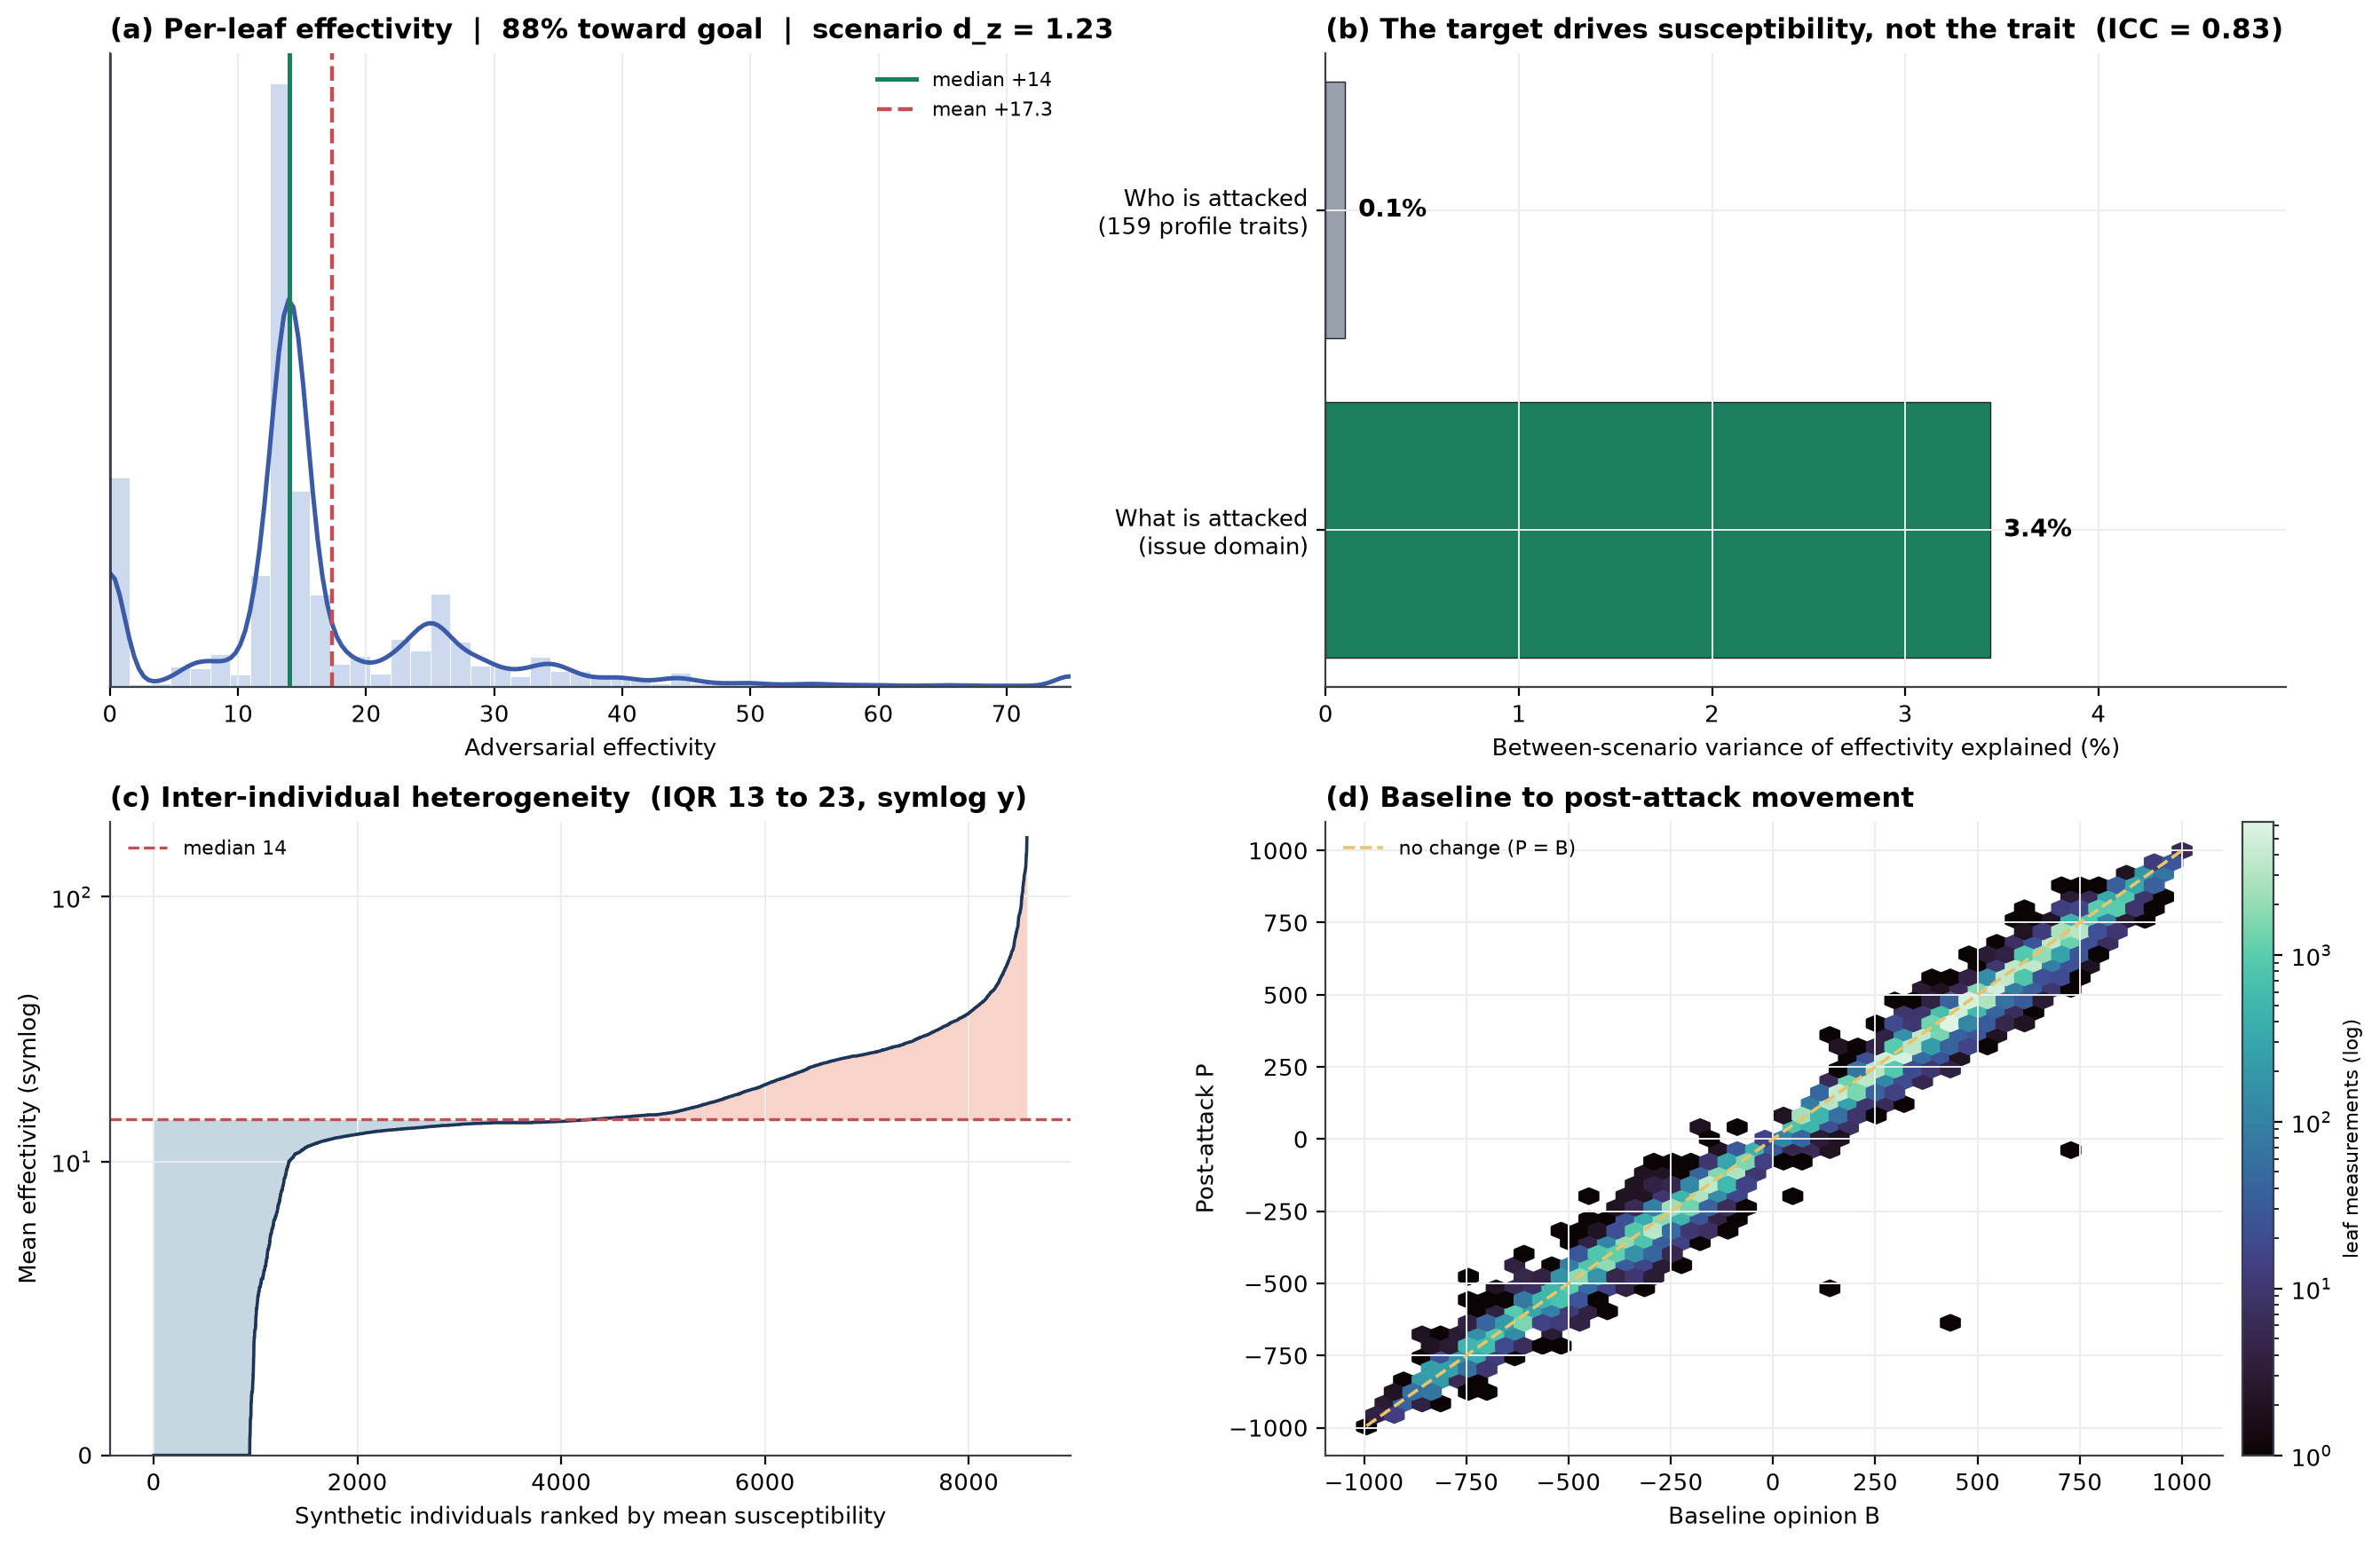
\includegraphics[width=0.92\linewidth]{../assets/figures/main/MAIN2_susceptibility_overview.png}
\apanote{(a)~Distribution of per-leaf adversarial effectivity; 88\% of measurements move toward
the attacker goal (median in teal, mean in red). (b)~Share of between-scenario effectivity
variance explained by what is attacked (issue domain, 3.4\%) versus who is attacked (the full
159-feature profile battery, 0.1\% out of sample), an approximately thirty-fold gap. (c)~Synthetic
individuals ranked by mean susceptibility (symmetric-log $y$): movability is strongly
heterogeneous between people (interquartile range 13 to 23, between-profile $SD \approx 14.7$).
(d)~Baseline opinion $B$ against post-attack opinion $P$ (log-density); the mass lies on the
attacker-intended side of the no-change diagonal. Values are on the 2,001-position bipolar opinion
scale.}
\end{figure}

\subsection{Variance Decomposition of Effectivity: Target Versus Profile}

A sharp asymmetry separates the two sources of variance an attacker could exploit. The issue
domain that is targeted explains 3.4\% of the between-scenario variance in mean effectivity,
whereas the entire 159-feature profile battery explains only 0.1\% out of sample, an approximately
thirty-fold gap (Figure~\ref{fig:overview}b). Knowing which opinion is attacked is thus far more
informative about how far it will move than knowing everything the profile records about the
person attacked. People are nonetheless not interchangeable: susceptibility is strongly
heterogeneous between individuals, with a between-profile intraclass correlation of
ICC(1) $= 0.83$, that is, 83\% of the leaf-level variance in effectivity lies between individuals
rather than within them, and a permutation test rejects exchangeability ($p = 0.001$). The
heterogeneity is large and stable (Figure~\ref{fig:overview}c) but largely orthogonal to what
standard trait inventories measure, a tension quantified in Section~\ref{sec:moderation}.

\subsection{Issue-domain Differences in Effectivity}

Movability is strongly opinion-dependent. A Kruskal-Wallis test across the six issue domains is
highly significant ($H = 579.1$, $p = 6.8\mathrm{e}{-123}$, $\varepsilon^2 = 0.067$;
Figure~\ref{fig:domains}A), and every domain is more movable than the least-movable reference
after false-discovery-rate correction. Two domains stand clearly above the rest: opinions about
critical infrastructure and energy sovereignty are the most movable (scenario-mean median $+19.0$),
followed by supranational and regional integration ($+16.8$); the remaining four domains cluster
together near $+13.5$ to $+14.3$ (Figure~\ref{fig:domains}B, Table~\ref{tab:domains}). The
rank-biserial effect size for the extreme contrast, critical infrastructure versus foreign policy,
reaches 0.46. The technocratic, instrumentally framed infrastructure and integration domains move
most, while the domains that anchor national identity and the integrity of democratic institutions
move least, a pattern consistent with motivated reasoning. Within every domain, however, individual
leaves range from highly movable to essentially inert (Figures~\ref{fig:s5} and \ref{fig:s6}), so
domain membership predicts movability only on average. The direction of the adversarial goal
carries no main effect: amplify and erode leaves do not differ in effectivity (Mann-Whitney
$p = 1.0$; Figure~\ref{fig:s6}c).

\begin{figure}[H]
\floatleft
\caption{Adversarial Effectivity by Issue Domain}
\label{fig:domains}
\vspace{2pt}
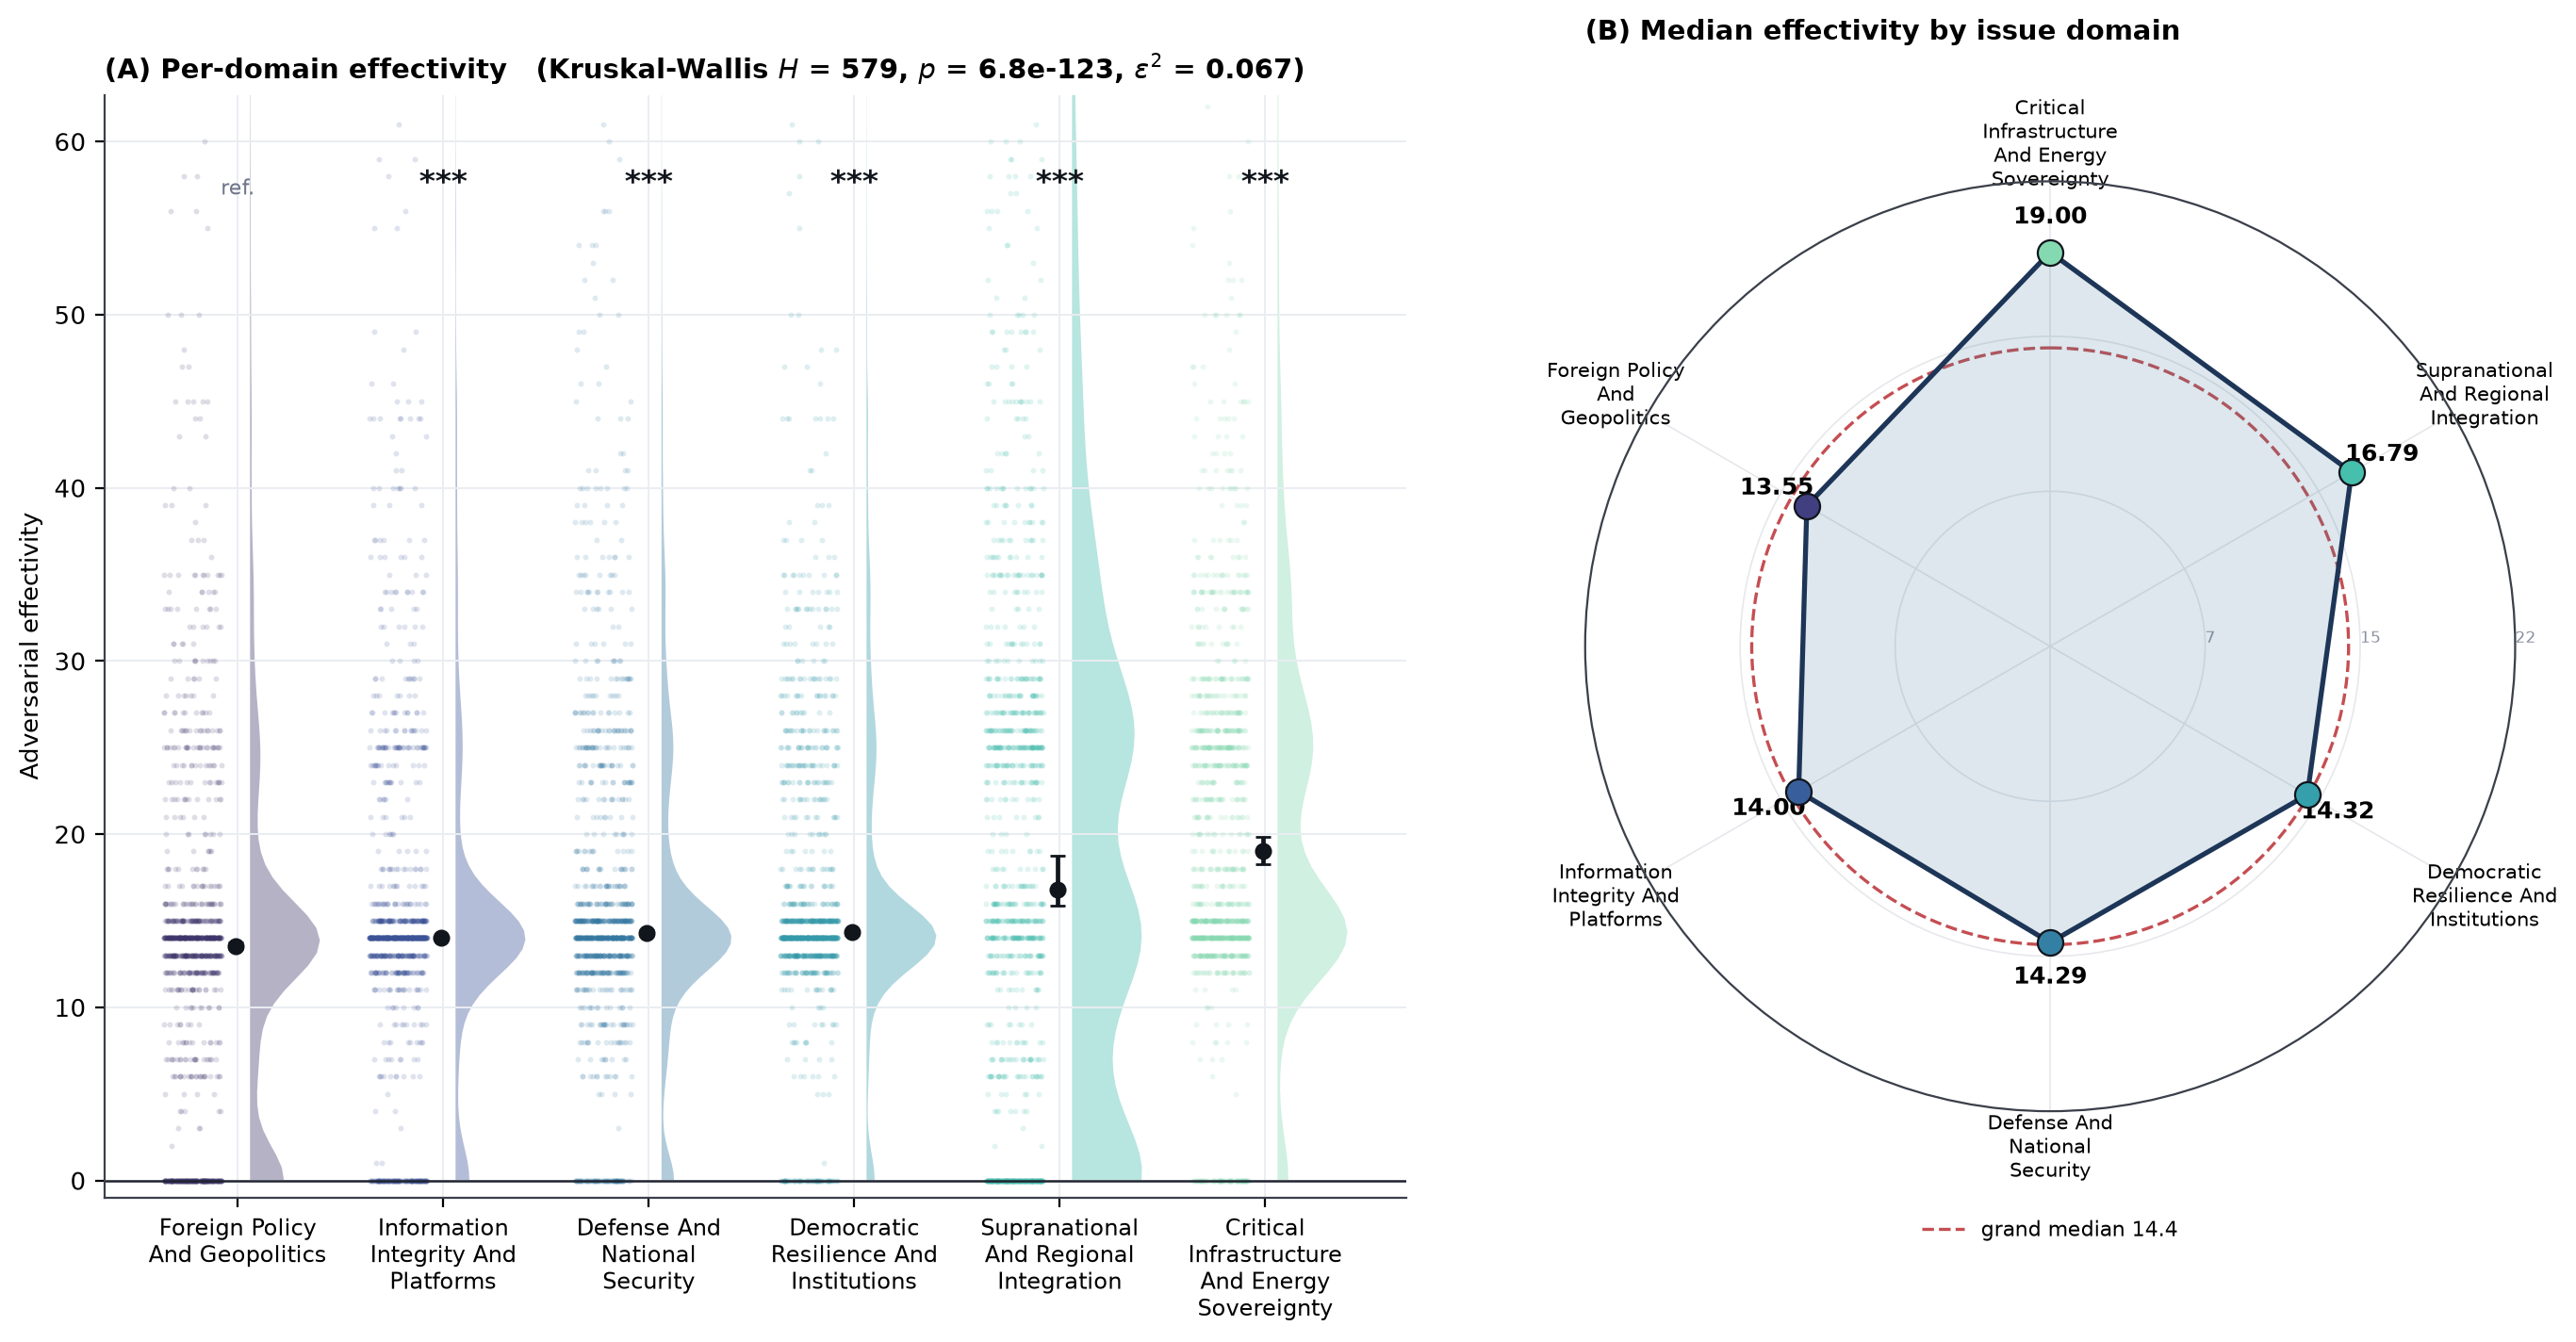
\includegraphics[width=0.97\linewidth]{../assets/figures/main/MAIN3_domain_susceptibility.png}
\apanote{(A)~Per-domain rainclouds (half-violin density, raw scenario points, and the
scenario-clustered median with a 95\% bootstrap confidence interval), ordered by movability with
the scenario-level Kruskal-Wallis omnibus in the panel header. Stars give each domain's
Mann-Whitney contrast against the least-movable reference domain (foreign policy) after
Benjamini-Hochberg correction, shown only where the rank-biserial effect also exceeds 0.10 so
that trivial large-sample differences are not flagged ($^{*}\,q<.05$, $^{**}\,q<.01$,
$^{***}\,q<.001$). (B)~Radar of the per-domain median effectivity, gradient-coloured, with the
dashed grand-median ring. Critical-infrastructure and supranational-integration opinions are the
most movable; the four remaining domains cluster lower.}
\end{figure}

\subsection{Effects of DISARM Operation Structure}

In contrast to the opinion target, the structure of the attack operation has little effect
(Figure~\ref{fig:attack}). Effectivity does not differ across the six DISARM Execute tactics
(Kruskal-Wallis $p = 0.54$) or across the four operation-complexity tiers ($p = 0.068$), and there
is no dose-response of effectivity on complexity (Spearman $\rho = -0.015$, $p = 0.16$). Only the
two Plan tactics differ, yet only marginally (planning around objectives versus target-audience
analysis; $p = 0.039$, rank-biserial $= 0.03$). The manipulation is therefore broadly effective
regardless of which operational variant delivers it. This bounds H3: the trait-matched-tactic
predictions require tactic families to differ in effectiveness so the difference can be moderated
by personality, and with essentially no tactic main effect to moderate, the specific matching
hypothesis is not supported at the level of DISARM tactic families. The trait directions that H3
shares with H2, neuroticism more movable and conscientiousness more resistant, do hold and are
reported next.

\begin{figure}[H]
\floatleft
\caption{Attack-phase Diagnostics Across the DISARM Operation Hierarchy}
\label{fig:attack}
\vspace{2pt}
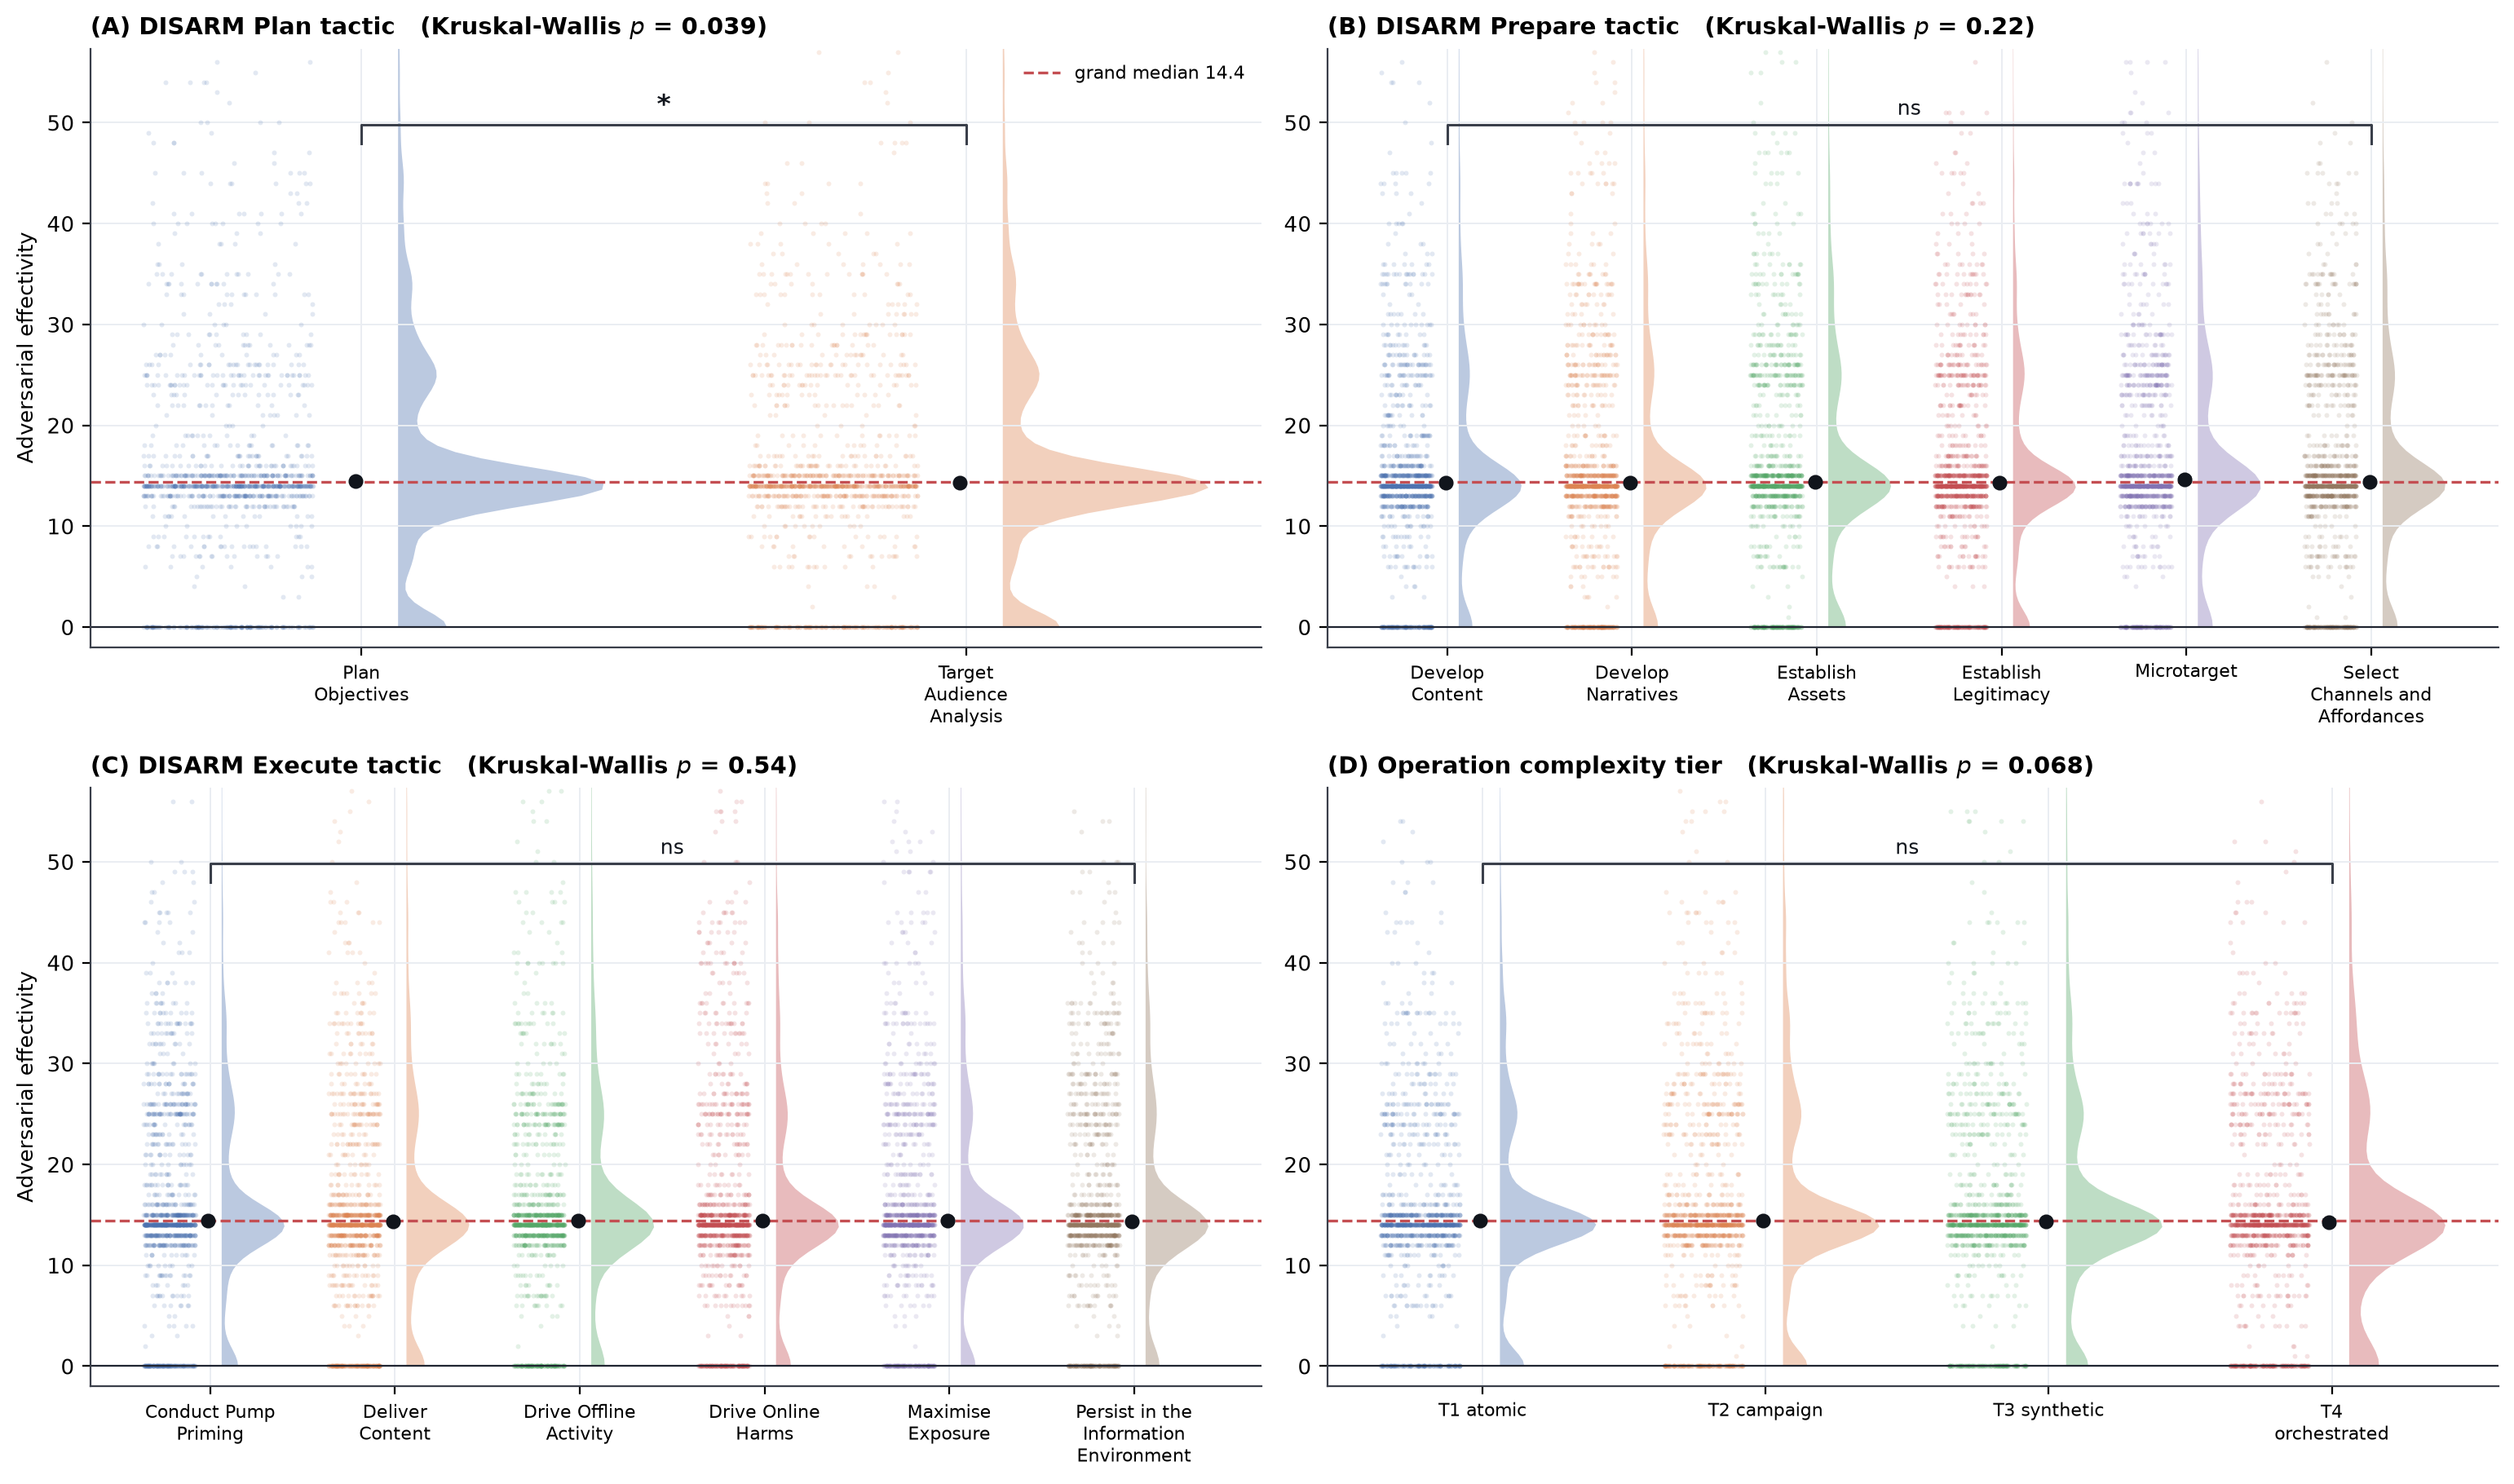
\includegraphics[width=0.92\linewidth]{../assets/figures/main/MAIN4_attack_phase_diagnostics.png}
\apanote{Adversarial effectivity by (A)~DISARM Plan tactic, (B)~Prepare tactic, (C)~Execute
tactic, and (D)~operation-complexity tier, each shown as rainclouds (half-violin density, raw
points, and the scenario-clustered median with 95\% confidence interval). The scenario-level
Kruskal-Wallis omnibus $p$ heads each panel. Only the two-level Plan tactic differs ($p = 0.039$);
Prepare, Execute, and complexity-tier contrasts are non-significant.}
\end{figure}

\subsection{Profile Moderation of Effectivity}\label{sec:moderation}

Although profiles differ markedly in susceptibility (ICC(1) $= 0.83$), the measured trait families
capture only a small part of that difference, in an interpretable order. Analysed each on its own
footing, the Big Five personality family carries the most signal (adjusted $R^2 = 0.32\%$ and the
only positive cross-validated $R^2$, $+0.0024$), ahead of political psychology (0.16\%), ideology
(0.06\%), moral foundations (0.03\%), and demographics (0.00\%); the full battery's cross-validated
$R^2$ is 0.0012 (Table~\ref{tab:moderation}, Figure~\ref{fig:moderation}a). General personality
therefore predicts susceptibility better than specific political attitudes do.

At the construct level, three Big Five traits survive the strict cross-family model with
false-discovery-rate control (Figure~\ref{fig:moderation}b, Table~\ref{tab:moderation}): openness
($\beta = +0.042$, 95\% CI $[0.020, 0.063]$, $q = 0.004$) and neuroticism ($\beta = +0.030$,
$[0.009, 0.050]$, $q = 0.040$) predict greater movability, and conscientiousness predicts resistance
($\beta = -0.035$, $[-0.055, -0.014]$, $q = 0.012$). Twenty-four traits are significant at the finer
facet level within their family. These directions match H2 and the phishing-vulnerability literature
\citep{lopezaguilar2025phishing,palmtims2025influence}: openness and neuroticism raise
susceptibility, conscientiousness lowers it. Their magnitudes are small, indicating that standard
trait axes capture only a minor, though real and sensible, part of who is movable. H2 is therefore
supported in direction but qualified in magnitude, and the political-psychology battery in particular
adds little beyond personality.

Re-estimating the construct moderators within each issue domain shows that the few sizeable trait
effects are domain-specific (Figure~\ref{fig:s7}, Table~\ref{tab:bydomain}): openness in the
information-integrity domain ($\beta = +0.101$, $q = 0.005$), political trust as a buffer in the
democratic-resilience domain ($\beta = -0.083$), and agreeableness alongside a traditionalist
orientation in foreign policy ($\beta = +0.068$ and $-0.075$). Finally, reliability bounds these
claims: under re-scoring by the primary model and across five independent providers the opinion
levels were reproducible whereas the signed per-item delta was substantially noisier
(Figures~\ref{fig:s1} to~\ref{fig:s3}), so the aggregate, direction-level findings are emphasised
over fine-grained per-scenario delta magnitudes.

\begin{figure}[H]
\floatleft
\caption{Person-level Moderators of Adversarial Effectivity}
\label{fig:moderation}
\vspace{2pt}
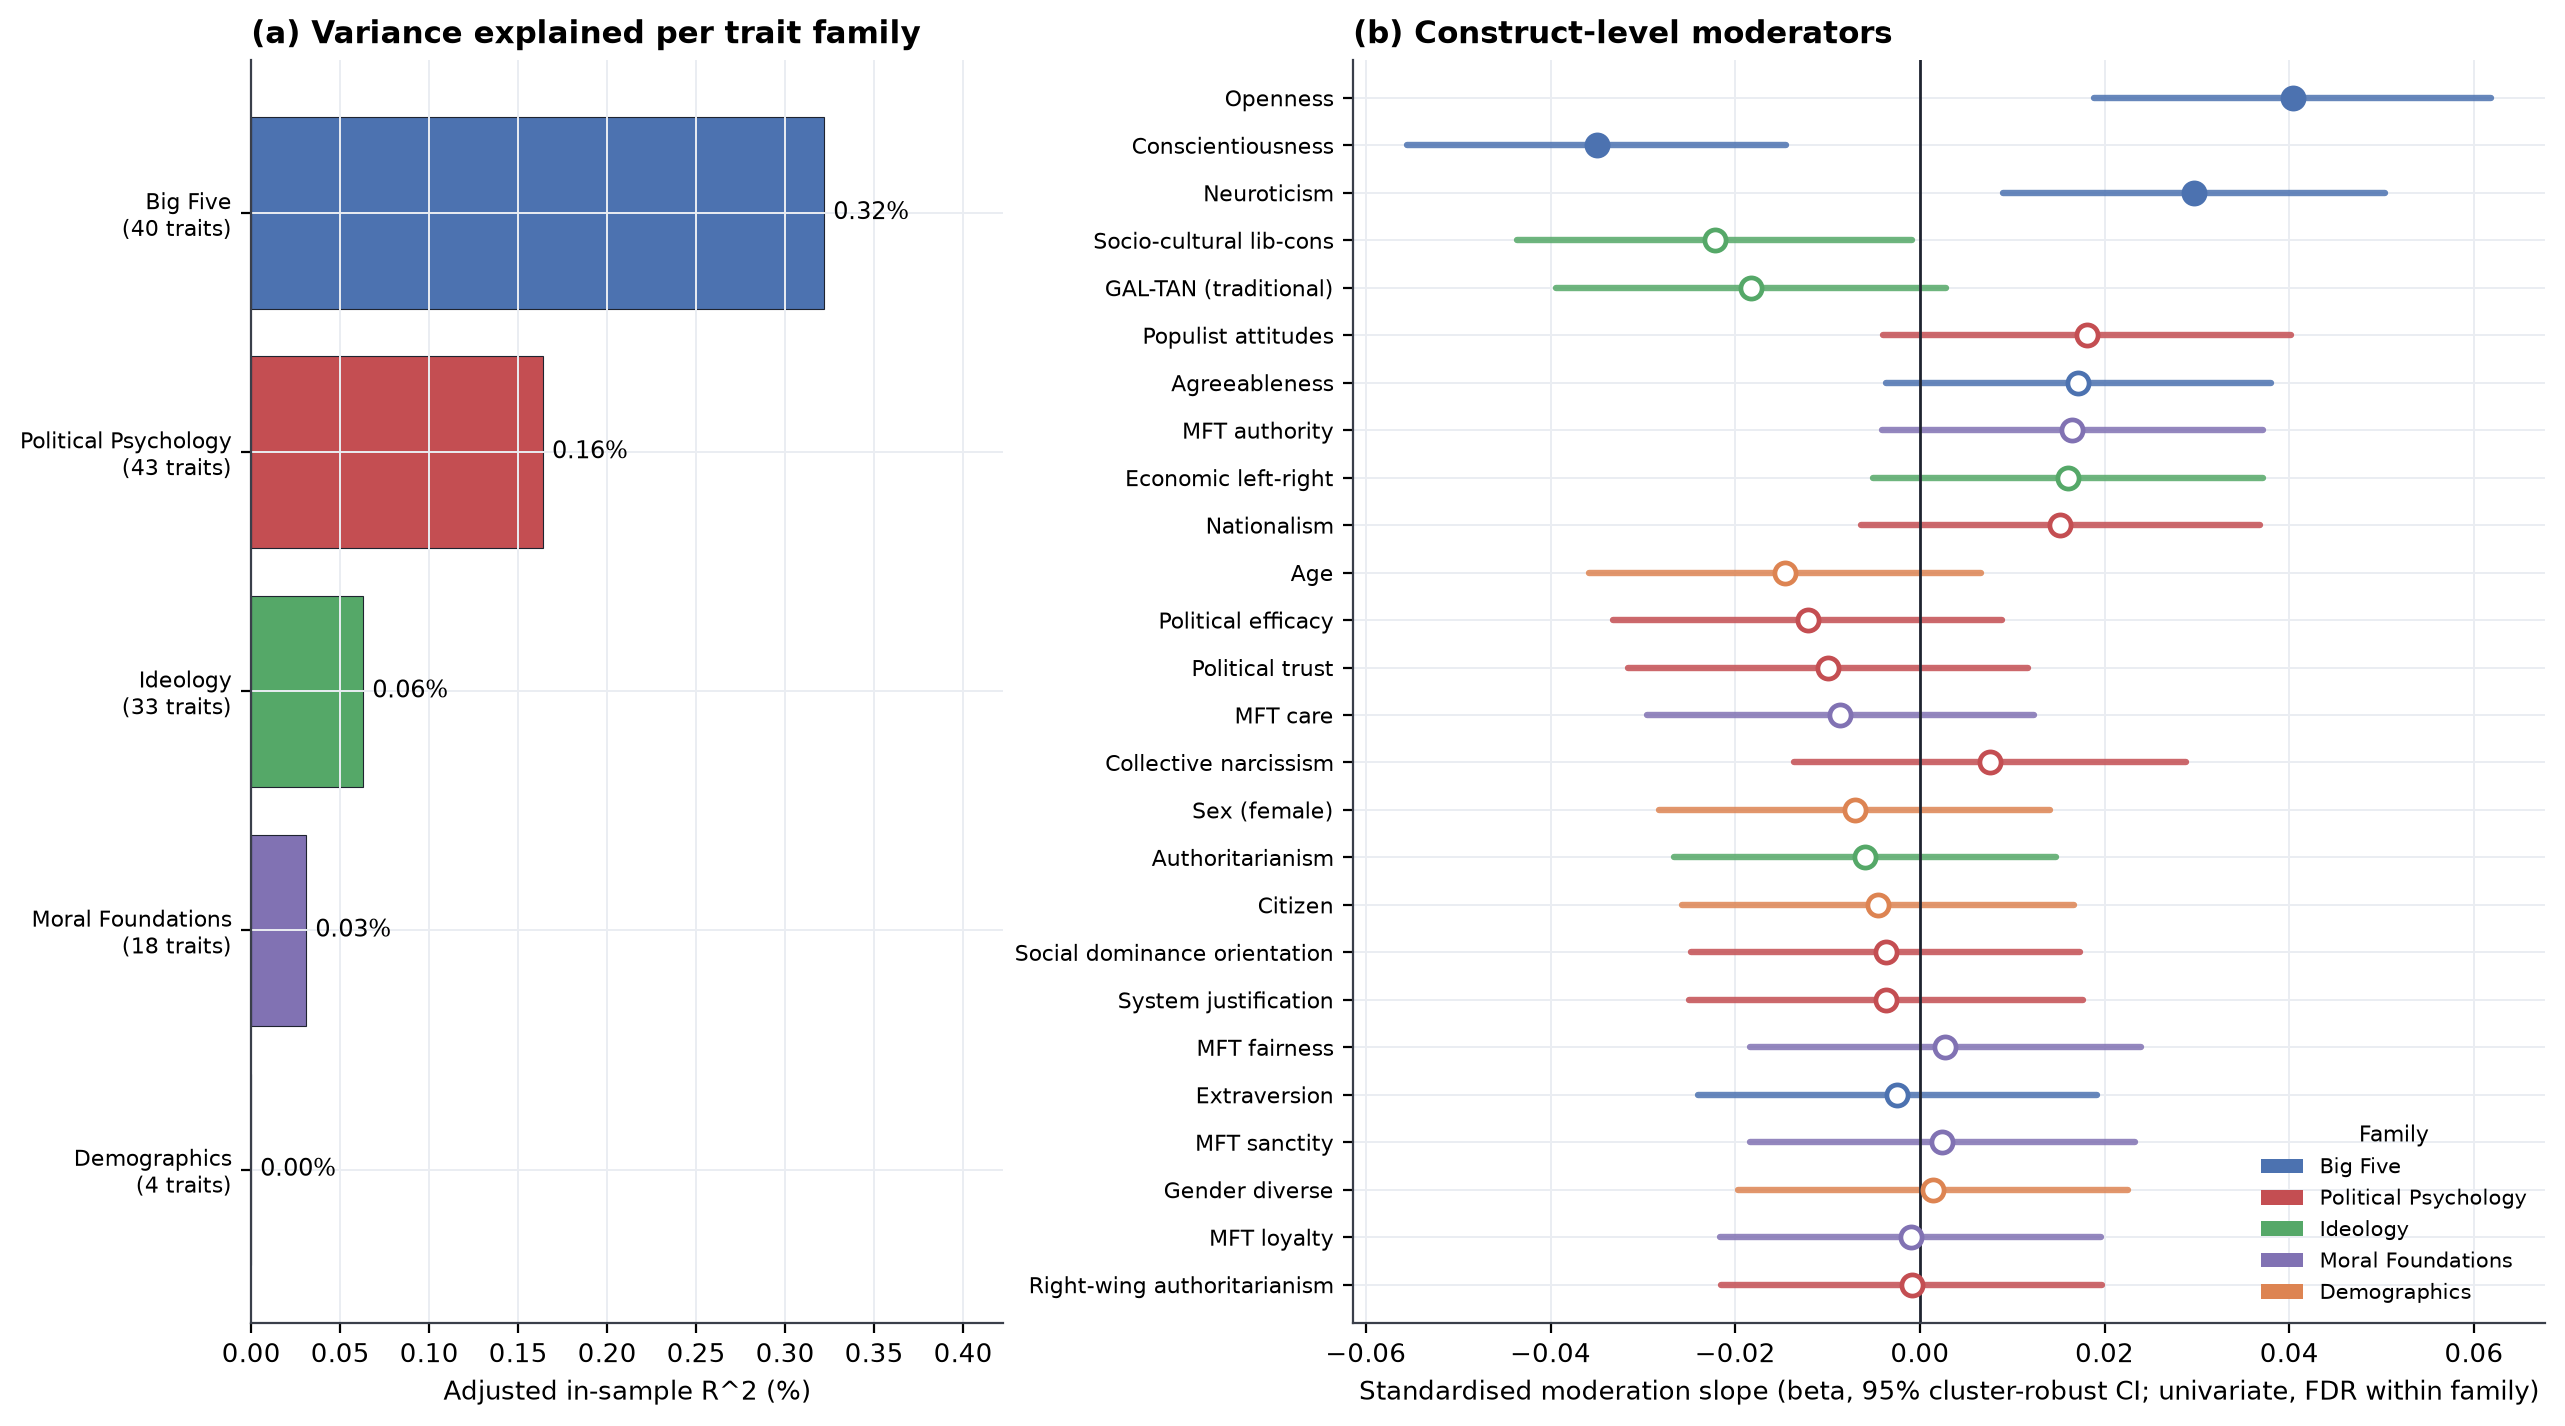
\includegraphics[width=0.97\linewidth]{../assets/figures/main/MAIN5_profile_moderation.png}
\apanote{(a)~Variance of susceptibility explained by each profile family (adjusted in-sample
$R^2$, non-negative). The Big Five carry the most signal, ahead of political psychology, ideology,
moral foundations, and demographics. (b)~Construct-level moderator forest, ordered by absolute
slope: univariate standardised slopes with 95\% cluster-robust confidence intervals,
false-discovery-rate corrected within family; filled markers are significant at $q<.05$ and colour
denotes trait family. Openness and neuroticism predict greater movability and conscientiousness
predicts resistance.}
\end{figure}

\begin{table}[H]
\floatleft
\caption{Profile Moderation: Family Predictive Signal and Significant Person-level Moderators}
\label{tab:moderation}
\vspace{2pt}
\begingroup\small
\begin{tabularx}{\linewidth}{@{}Yccccc@{}}
\multicolumn{6}{@{}l}{\textit{Panel A. Variance explained by trait family}}\\
\toprule
Profile family & Traits ($k$) & Adj. $R^2$ (\%) & \multicolumn{2}{c}{CV $R^2$} & \\
 & & & Standalone & Unique & \\
\midrule
Big Five & 40 & 0.322 & $+0.0024$ & $+0.0029$ & \\
Political Psychology & 43 & 0.164 & $-0.0014$ & $0.0000$ & \\
Ideology & 33 & 0.063 & $-0.0006$ & $0.0000$ & \\
Moral Foundations & 18 & 0.031 & $-0.0017$ & $0.0000$ & \\
Demographics & 4 & 0.000 & $-0.0011$ & $0.0000$ & \\
\bottomrule
\end{tabularx}

\vspace{5pt}
\begin{tabularx}{\linewidth}{@{}Yp{2.0cm}p{2.8cm}p{1.4cm}Y@{}}
\multicolumn{5}{@{}l}{\textit{Panel B. Significant cross-family moderators (OLS, HC3,
BH-FDR $q<.05$)}}\\
\toprule
Moderator & $\beta_{\text{std}}$ & 95\% CI & $q$ & Direction \\
\midrule
Openness & $+0.042$ & $[+0.020, +0.063]$ & .004 & More movable \\
Conscientiousness & $-0.035$ & $[-0.055, -0.014]$ & .012 & More resistant \\
Neuroticism & $+0.030$ & $[+0.009, +0.050]$ & .040 & More movable \\
\bottomrule
\end{tabularx}
\endgroup
\apanote{Panel A: adjusted in-sample $R^2$ is non-negative; standalone and unique cross-validated
(CV) $R^2$ are five-fold ridge estimates, with unique variance the drop in full-model CV $R^2$
when the family is removed. The full-battery CV $R^2$ is 0.0012. Panel B: standardised slopes from
a single cross-family ordinary-least-squares model with HC3 robust standard errors; 3 of 26 curated
constructs survive false-discovery-rate control, all from the Big Five.}
\end{table}

\subsection{Profile Predictors of Direct and Network-Conditioned Susceptibility}
\label{sec:profile-network-bridge}

The preceding section shows that standard profile traits capture only a small part of private
adversarial effectivity. The exposure-network layer asks a related but distinct question: whether
the profiles that are more susceptible in isolation are also the profiles whose opinions are most
amplified after network exposure. To answer this, each profile was summarised across the 35
opinion-by-attack condition cells in the network experiment, yielding one profile-level mean for
direct private susceptibility, \(\mathrm{AE}_{\mathrm{private}}=(P-B)d\), and one profile-level mean
for post-network amplification, \((N^P-P)d\). The unit of inference in this analysis is therefore
the profile (\(n=100\)), not the scenario row.

Direct private susceptibility and post-network amplification were positively but only moderately
associated (Figure~\ref{fig:profile-network-bridge}a), \(r=.28\), 95\% bootstrap CI
\([.08,.47]\). Thus, profiles that moved more strongly after the private attack also tended to show
larger network-conditioned amplification, but the relationship was far from deterministic. The
network increment is therefore not simply a restatement of private movability.

The same pattern appears in the profile-predictor models (Figure~\ref{fig:profile-network-bridge}b).
The direct and network-conditioned coefficient profiles overlapped, but they did not coincide.
Neuroticism predicted both direct susceptibility and post-network amplification. Openness was more
strongly tied to the direct private effect, whereas conscientiousness, extraversion, and
agreeableness were more pronounced in the network-increment model. This suggests that exposure to
peer context preserves part of the individual susceptibility structure while introducing an
additional social-context-dependent component.

The strongest evidence for this distinction comes from the direct-adjusted network model
(Figure~\ref{fig:profile-network-bridge}c). Direct susceptibility alone explained 7.8\% of the
profile-level variation in post-network amplification. The profile-trait model explained 30.0\%.
Adding direct susceptibility to the trait model increased explained variance only from
\(R^2=.300\) to \(R^2=.301\). In that adjusted model, direct susceptibility was no longer a
meaningful predictor of post-network amplification, \(\beta=.043\), 95\% HC3 CI
\([-.207,.293]\), \(p=.736\). Together, these results support H5: private susceptibility and
post-network amplification shared a moderate profile-level association, but network-conditioned
susceptibility was not reducible to private susceptibility once profile traits were modelled
jointly. This result motivates the next analysis: if network exposure creates a distinct
susceptibility component, then the network-wide effect of an attack should depend on where
susceptible or resilient profiles are positioned in the exposure graph.

\begin{figure}[H]
\floatleft
\caption{Network-Conditioned Susceptibility Is Not Reducible to Direct Private Susceptibility}
\label{fig:profile-network-bridge}
\vspace{2pt}
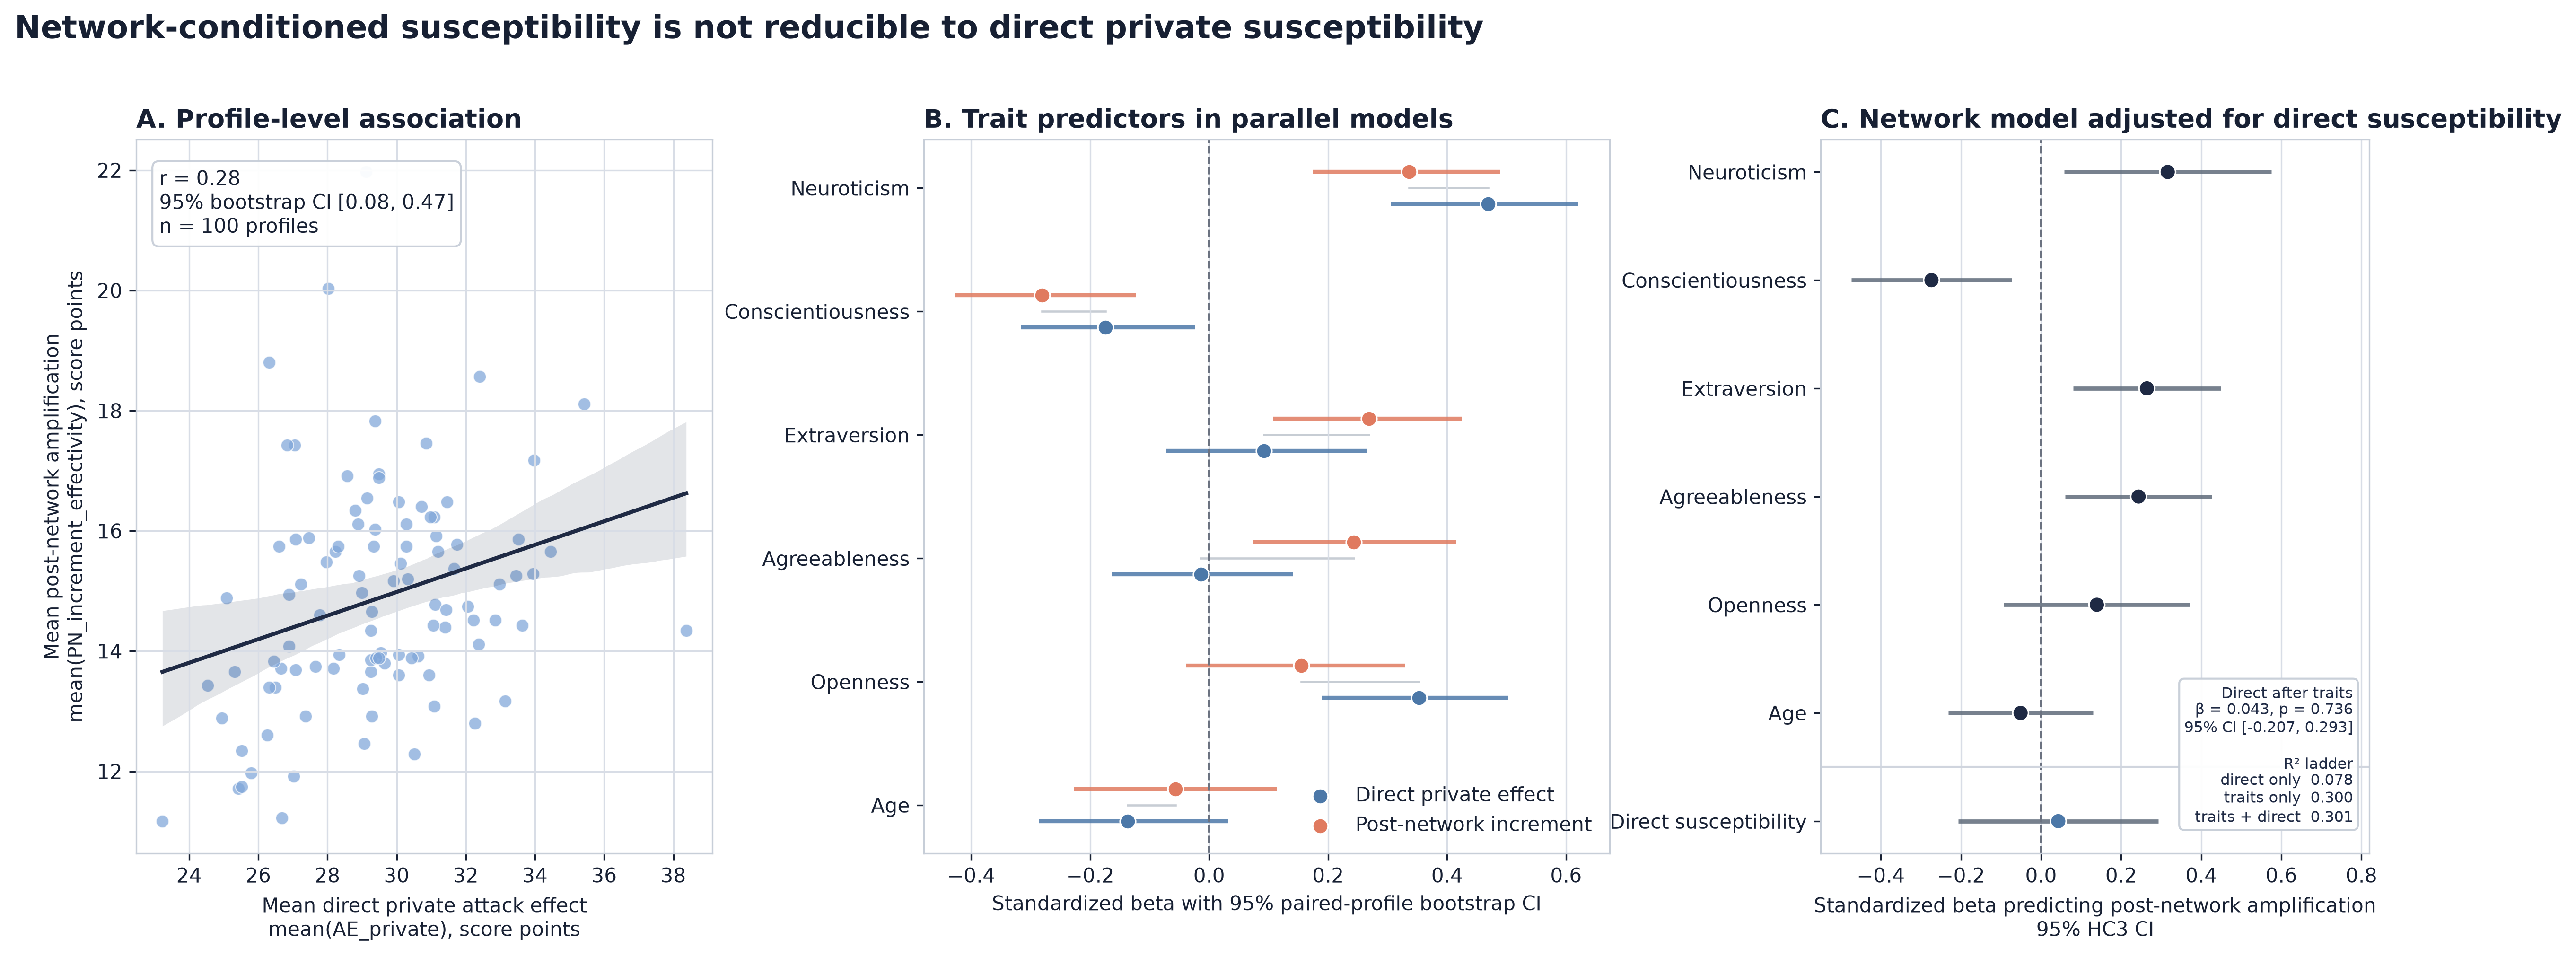
\includegraphics[width=0.99\linewidth]{../assets/figures/main/MAIN6_profile_direct_vs_network.png}
\apanote{Each point in Panel A is one profile (\(n=100\)), averaged across the 35
opinion-by-attack condition cells. Direct susceptibility is
\(\mathrm{AE}_{\mathrm{private}}=(P-B)d\). Post-network amplification is \((N^P-P)d\), where
\(B\) is the private baseline, \(P\) the private post-attack opinion, \(N^P\) the post-attack
opinion after network exposure, and \(d\) the adversarial direction. Panel A uses score-point means
and paired-profile bootstrap uncertainty. Panels B and C use standardised outcomes and predictors;
models adjust for sex indicators. Panel B shows paired-profile bootstrap confidence intervals, and
Panel C shows HC3 robust confidence intervals. Positive values indicate movement in the
attack-aligned direction.}
\end{figure}

\subsection{Influential Sender Positions Convert Private Susceptibility Into Network Amplification}
\label{sec:network-results}

We finally tested whether private susceptibility becomes more consequential when it is located at
influential positions in the exposure graph. The fixed-position production run used one
profile-position mapping and therefore described the network response under that realised
assignment. However, that mapping produced only limited variation in the alignment between private
susceptibility and sender reach. To test H6 and H7 more directly, we used the counterfactual
alignment design described in Section~\ref{sec:network-method}: the same profiles, opinion targets,
attack vectors, and empirical graph were held fixed, while the assignment between profiles and
network positions was varied across 35 opinion $\times$ attack condition cells.

The alignment manipulation behaved as intended. Across the 35 condition cells, each summarising the
same 100 profiles, planned and achieved alignment were almost perfectly matched
($r=0.9999$), with a maximum absolute target error of 0.027 and an achieved-alignment range from
$-0.892$ to $+0.920$. Negative alignment means that comparatively resilient profiles occupied
higher-reach positions; positive alignment means that comparatively susceptible profiles occupied
higher-reach positions. In the most resilient high-reach conditions, the top-20 sender positions
had a mean private-susceptibility $z$ score of approximately $-1.16$; in the most susceptible
high-reach conditions, the corresponding mean was approximately $+1.16$.

\begin{figure}[H]
\floatleft
\caption{Private Susceptibility Becomes Network-consequential When It Aligns With Sender Reach}
\label{fig:network-amplification}
\vspace{2pt}
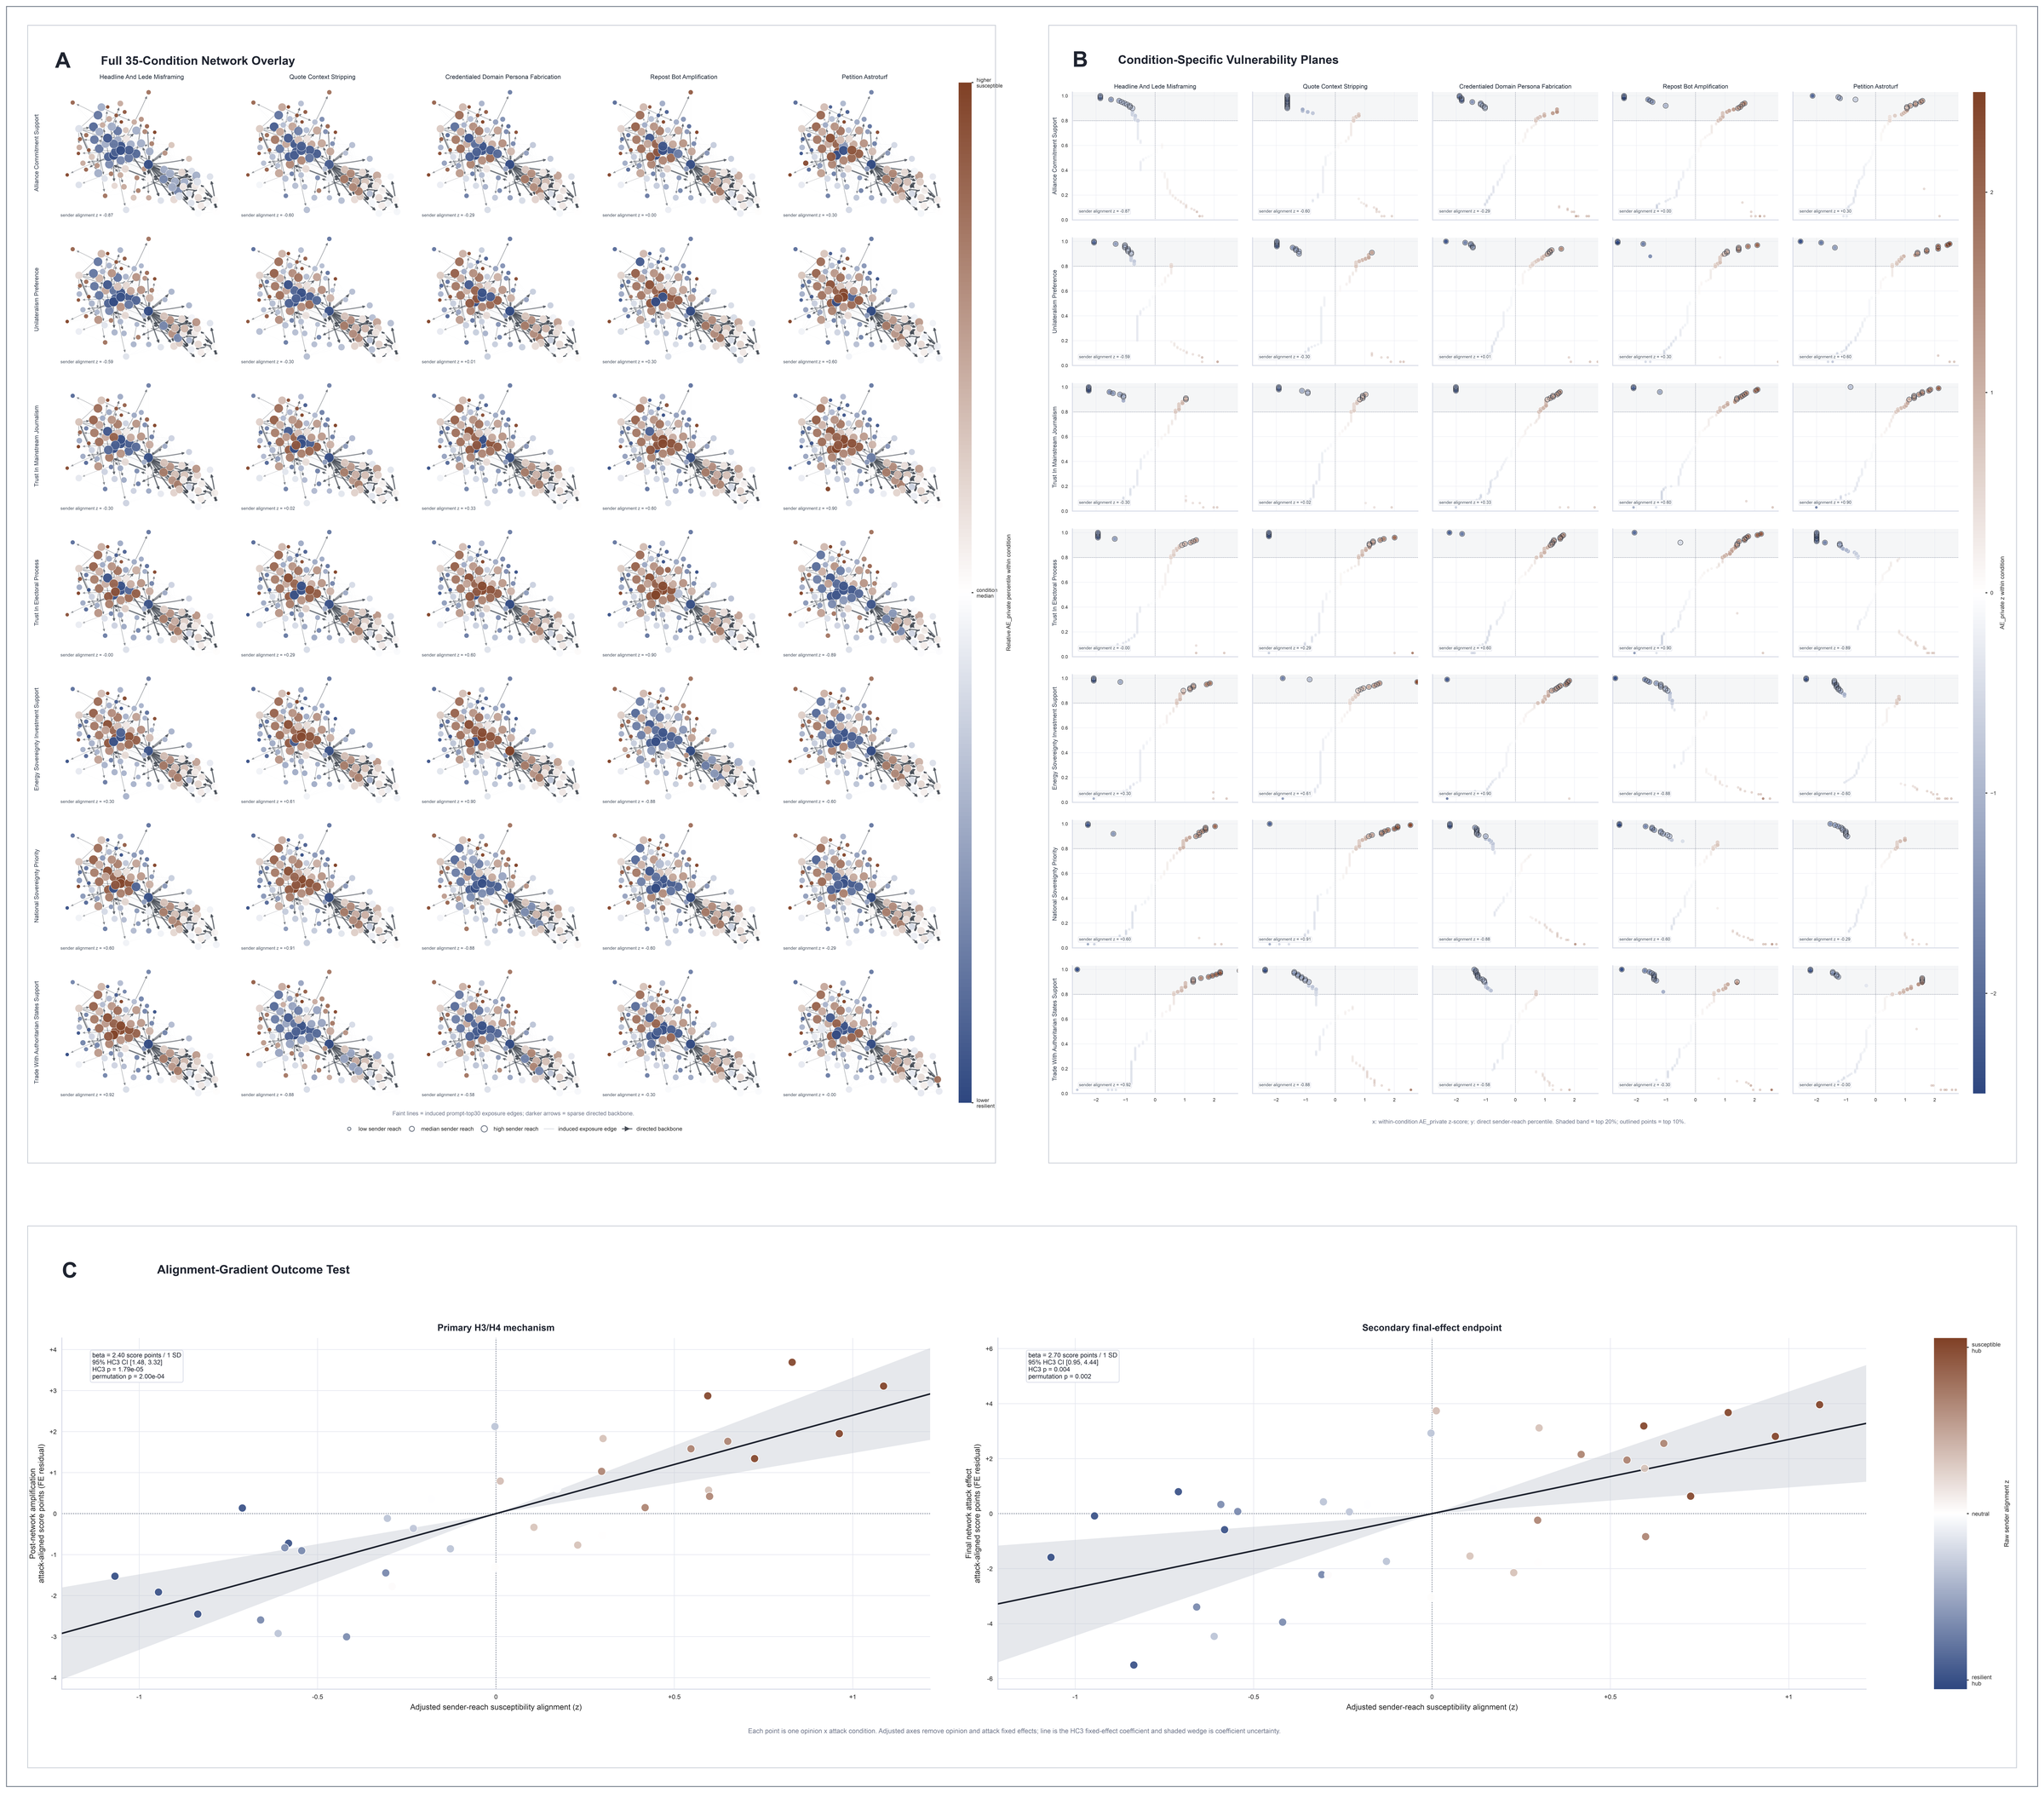
\includegraphics[width=0.98\linewidth]{../assets/figures/main/MAIN7_susceptibility_network_amplification_.png}
\apanote{Panel A overlays the empirical exposure graph across all 35 condition cells; node colour
shows within-condition private susceptibility, \(\mathrm{AE}^{\mathrm{private}}=(P-B)d\), node
size shows direct sender reach, \(R_p=\sum_q w_{pq}\), and directed edges run from visible sender
positions to exposed receiver positions. Panel B shows the corresponding condition-specific
vulnerability planes, with private-susceptibility position on the horizontal axis and sender-reach
position on the vertical axis. Panel C shows the condition-level fixed-effect outcome test. Each
point is one opinion $\times$ attack condition cell averaging 100 profiles. The left outcome is
post-network amplification, \(\mathrm{mean}((N^P-P)d)\); the right outcome is total network attack
effect, \(\mathrm{mean}((N^P-B)d)\). Axes in Panel C are residualised for opinion and attack fixed
effects. The shaded wedges show HC3 coefficient uncertainty for the alignment slope, not prediction
intervals.}
\end{figure}

Figure~\ref{fig:network-amplification} shows the mechanism visually. Panels A and B confirm that
the empirical exposure substrate is held fixed while susceptibility is redistributed across
network influence. Panel C then estimates whether the achieved condition-level alignment,
\(A_c\), predicts stronger network amplification after removing opinion and attack fixed effects.
For the primary endpoint, post-network amplification \(\mathrm{mean}((N^P-P)d)\), the alignment
slope was positive and large: \(\beta=2.399\) score points per one-standard-deviation increase in
alignment, with HC3 95\% CI \([1.478,3.320]\), \(p=1.79\mathrm{e}{-05}\), and directional
within-attack permutation \(p=0.00020\). Moving from \(A_c=-0.9\) to \(A_c=+0.9\) therefore
corresponds to an estimated increase of 4.32 attack-aligned score points in post-network
amplification.

The secondary endpoint, total network attack effect \(\mathrm{mean}((N^P-B)d)\), showed the same
direction. The fixed-effect slope was \(\beta=2.697\), with HC3 95\% CI \([0.953,4.440]\),
\(p=0.00398\), and directional within-attack permutation \(p=0.00200\). Across the same alignment
range from \(-0.9\) to \(+0.9\), this implies an estimated increase of 4.85 attack-aligned score
points in the final network-conditioned attack effect.

These results support H6 and H7 as complementary sides of the same network mechanism. H6 is
supported because network-wide attack effects increased when comparatively susceptible profiles
occupied higher-reach sender positions. H7 is supported because negative-alignment conditions, in
which comparatively resilient profiles occupied those higher-reach positions, attenuated the
network-wide effect. This should be interpreted as a controlled network-mechanism test, not as a
claim that real platforms naturally assign susceptible users to influential positions.

\section{Discussion}

\subsection{Main Findings}

\noindent\textit{[Placeholder. To be completed.]}

\subsection{Limitations}

Several limitations bound the interpretation of these results, the most fundamental being one
of coverage. The 10,000 scenarios sample a negligible fraction of the joint state space from
which they are drawn: the filtered attack ontology alone admits 48,991 triplets, and crossing
these against the 106 directional opinion leaves already yields on the order of five million
attack-by-opinion configurations before any profile variation is considered. Because profiles
are assigned bijectively, no synthetic person recurs, so within any fixed attack-by-opinion
cell the sample available for estimating higher-order interactions is effectively one.
Factor-level attribution, such as identifying which specific Plan, Prepare, and Execute triplet
is most effective for a given personality on a given target, is therefore not licensed by the
present data. This is a deliberate trade: the maximum-entropy design prioritises breadth over
within-cell depth, which is the appropriate choice for a first survey of a previously unmapped
space, but it defers fine-grained interaction hypotheses to a targeted factorial follow-up with
planned replication.

The weak profile moderation invites a related caution. The full 159-feature battery explains
almost no out-of-sample variance (cross-validated $R^2 = 0.001$), which admits two
non-exclusive readings. The first is substantive: opinion-domain membership explains roughly
thirty times more between-scenario variance ($R^2 = 0.034$), and the high between-profile
ICC(1) of 0.83 indicates that susceptibility is strongly person-specific yet poorly aligned
with the constructs standard inventories encode. The second is a power-and-design artefact,
because maximum-entropy sampling favours coverage over dense representation of trait-defined
subgroups, so the extreme-trait profiles that carry the most leverage for slope estimation
appear only in proportion to their share of the space rather than being oversampled.
Attenuation toward zero is thus expected even where true effects exist. Consistent with this,
exploratory runs that restricted the prompt to the personality and demographic subset, holding
attack and opinion content fixed, recovered moderation of moderate magnitude. The three Big
Five moderators that survive correction at small slopes ($|\beta| = 0.030$ to $0.042$) are
accordingly better read as lower bounds than as overfitted noise.

Part of this attenuation may originate in the measurement instrument itself. Each agent call
presents roughly 159 profile features, a three-phase DISARM triplet, and a full opinion cluster
at once, and the primary model is run without reasoning traces, a choice that stabilises strict
JSON scoring but removes the stepwise integration that a prompt of this density arguably
requires. It is not established that a large mixture-of-experts model differentially weights
individual lower-order constructs, such as specific Big Five facets or narrow ideology
subscales, when it must return a numeric score for every leaf under this load. The subset tests
noted above are consistent with such dilution, since trait-relevant signal that the
full-profile condition suppressed re-emerged once the surrounding profile content was removed.
Whether the mechanism is context saturation, signal dilution, or a prompt-engineering artefact
cannot be settled without systematic ablation across prompt-density levels, and the concern
bears most directly on the null results for the political-psychology, ideology, and
moral-foundations families, whose effects depend on integrating fine-grained attitudinal
context.

A further constraint follows from holding the instrument fixed. Scoring every scenario with a
single model family removes model identity as a hidden moderator but replicates that model's
idiosyncrasies across the whole dataset without dilution. Re-scoring a held-out subset with five
independent providers showed that opinion levels were moderately reproducible (baseline and
post-attack ICC(A,1) of 0.57 and 0.43) whereas the signed effectivity delta was not
(ICC(A,1) $= 0.01$, mean pairwise Spearman $= 0.12$). This gap is expected, because a
direction-adjusted difference amplifies level noise, but it implies that part of the
between-scenario effectivity variance, and of the apparent moderation gradients, may track the
primary model's scoring tendencies rather than stable properties of the profiles, attacks, or
opinions. The aggregate and directional findings, such as the sign of the significant
moderators and the movability ordering of the issue domains, are therefore treated as more
dependable than individual scenario-level magnitudes, with cross-model replication the proper
standard for confirmation.

These instrument-level concerns sharpen a more basic one about construct validity. The design
assumes that an LLM agent conditioned on a synthetic profile is an adequate proxy for a human
respondent under adversarial influence. Population-level evidence supports such proxies for
survey opinion \citep{argyle2023out}, and LLM-authored appeals shift human attitudes comparably
to lay-authored ones \citep{bai2025llm}, yet the present use is more demanding, requiring the
agent to infer both a plausible opinion state from a high-resolution profile and its
direction-aware shift under a structured operation. Probing the internal geometry of a large
language model is not equivalent to eliciting the meta-analytic response of a human population:
the model may generate opinion adjustments through surface-level consistency heuristics rather
than through the motivated reasoning, identity-protective cognition, and source-credibility
judgements that govern human persuasion, and its internal representation of
personality-opinion covariation has not been shown to match the human one for this task. Such
a gap could inflate mean effectivity, consistent with the 89\,percent movement rate, and could
distort the trait gradients. The estimates are accordingly read as simulation-internal
directional predictions, and validation in human samples remains the necessary next step.

A final limitation anticipates the network layer reported in the next section. Its exposure
graph is derived from a political-discourse subset of the BlueSky platform, whose political user
base is concentrated in particular demographic and ideological communities and whose recorded
ties capture following and reply relations rather than the verified content co-exposure that
actually drives opinion diffusion. Whether the topology and community structure of this
substrate generalise to mass-reach platforms or to offline contexts is unestablished, so the
external validity of the network-layer conclusions is bounded by how representative BlueSky is
of social interaction in the wider information environment.

\subsection{Future Directions}

\noindent\textit{[Placeholder. To be completed.]}

\section{Conclusion}

\noindent\textit{[Placeholder. To be completed.]}

\clearpage
\begin{thebibliography}{99}
\setlength{\itemsep}{0.45em}

\bibitem[Argyle et~al.(2023)]{argyle2023out}
Argyle, L. P., Busby, E. C., Fulda, N., Gubler, J. R., Rytting, C., \& Wingate, D. (2023). Out of
one, many: Using language models to simulate human samples. \textit{Political Analysis, 31}(3),
337-351. \doiurl{10.1017/pan.2023.2}

\bibitem[Bada \& Nurse(2020)]{bada2020social}
Bada, M., \& Nurse, J. R. C. (2020). The social and psychological impact of cyber-attacks. In
\textit{Emerging Cyber Threats and Cognitive Vulnerabilities} (pp. 73-92). Academic Press.
\doiurl{10.1016/B978-0-12-816203-3.00004-6}

\bibitem[Bai et~al.(2025)]{bai2025llm}
Bai, H., Voelkel, J. G., Muldowney, S., Eichstaedt, J. C., \& Willer, R. (2025). LLM-generated
messages can persuade humans on policy issues. \textit{Nature Communications, 16}, Article 6037.
\doiurl{10.1038/s41467-025-61345-5}

\bibitem[Bail et~al.(2018)]{bail2018exposure}
Bail, C. A., Argyle, L. P., Brown, T. W., Bumpus, J. P., Chen, H., Fallin Hunzaker, M. B., Lee, J.,
Mann, M., Merhout, F., \& Volfovsky, A. (2018). Exposure to opposing views on social media can
increase political polarization. \textit{Proceedings of the National Academy of Sciences,
115}(37), 9216-9221. \doiurl{10.1073/pnas.1804840115}

\bibitem[Benjamini \& Hochberg(1995)]{benjamini1995controlling}
Benjamini, Y., \& Hochberg, Y. (1995). Controlling the false discovery rate: A practical and
powerful approach to multiple testing. \textit{Journal of the Royal Statistical Society: Series B
(Methodological), 57}(1), 289-300. \doiurl{10.1111/j.2517-6161.1995.tb02031.x}

\bibitem[Bond et~al.(2012)]{bond2012experiment}
Bond, R. M., Fariss, C. J., Jones, J. J., Kramer, A. D. I., Marlow, C., Settle, J. E., \& Fowler,
J. H. (2012). A 61-million-person experiment in social influence and political mobilization.
\textit{Nature, 489}(7415), 295-298. \doiurl{10.1038/nature11421}

\bibitem[Botes(2023)]{botes2023autonomy}
Botes, M. (2023). Autonomy and the social dilemma of online manipulative behavior. \textit{AI and
Ethics, 3}(1), 315-323. \doiurl{10.1007/s43681-022-00157-5}

\bibitem[Cameron et~al.(2008)]{cameron2008bootstrap}
Cameron, A. C., Gelbach, J. B., \& Miller, D. L. (2008). Bootstrap-based improvements for inference
with clustered errors. \textit{The Review of Economics and Statistics, 90}(3), 414-427.
\doiurl{10.1162/rest.90.3.414}

\bibitem[Cioffi-Revilla(2002)]{cioffirevilla2002invariance}
Cioffi-Revilla, C. (2002). Invariance and universality in social agent-based simulations.
\textit{Proceedings of the National Academy of Sciences, 99}(suppl.\ 3), 7314-7316.
\doiurl{10.1073/pnas.082081499}

\bibitem[Council of the European Union(2025)]{councileu2025cyber}
Council of the European Union. (2025, June 30). \textit{Cyber threats in the EU: Facts and figures}
(ENISA 2024). \url{https://www.consilium.europa.eu/en/policies/top-cyber-threats/}

\bibitem[Cummins(2025)]{cummins2025threat}
Cummins, J. (2025). \textit{The threat of analytic flexibility in using large language models to
simulate human data} [Preprint]. arXiv. \doiurl{10.48550/arXiv.2509.13397}

\bibitem[Decker \& Kr\"amer(2023)]{decker2023personality}
Decker, H., \& Kr\"amer, N. (2023). Is personality key? Persuasive effects of prior attitudes and
personality in political microtargeting. \textit{Media and Communication, 11}(3), 250-261.
\doiurl{10.17645/mac.v11i3.6627}

\bibitem[DISARM Foundation(2023)]{disarmfoundationnd}
DISARM Foundation. (2023). \textit{DISARM Red framework}.
\url{https://www.disarm.foundation/framework}

\bibitem[ENISA(2023)]{enisa2023elections}
European Union Agency for Cybersecurity. (2023, October 19). \textit{EU elections at risk with rise
of AI-enabled information manipulation}.
\url{https://www.enisa.europa.eu/news/eu-elections-at-risk-with-rise-of-ai-enabled-information-manipulation}

\bibitem[ENISA \& EEAS(2022)]{enisaeeas2022fimi}
European Union Agency for Cybersecurity, \& European External Action Service. (2022).
\textit{Foreign information manipulation and interference (FIMI) and cybersecurity: Threat
landscape}. ENISA. \doiurl{10.2824/930829}

\bibitem[Hoerl \& Kennard(1970)]{hoerl1970ridge}
Hoerl, A. E., \& Kennard, R. W. (1970). Ridge regression: Biased estimation for nonorthogonal
problems. \textit{Technometrics, 12}(1), 55-67. \doiurl{10.1080/00401706.1970.10488634}

\bibitem[Hutchins et~al.(2011)]{hutchins2011intelligence}
Hutchins, E. M., Cloppert, M. J., \& Amin, R. M. (2011). Intelligence-driven computer network
defense informed by analysis of adversary campaigns and intrusion kill chains. \textit{Leading
Issues in Information Warfare \& Security Research, 1}(1), 80-106.

\bibitem[Inkster et~al.(2023)]{inkster2023cybersecurity}
Inkster, B., Knibbs, C., \& Bada, M. (2023). Cybersecurity: A critical priority for digital mental
health. \textit{Frontiers in Digital Health, 5}, Article 1242264.
\doiurl{10.3389/fdgth.2023.1242264}

\bibitem[Isaak \& Hanna(2018)]{isaak2018user}
Isaak, J., \& Hanna, M. J. (2018). User data privacy: Facebook, Cambridge Analytica, and privacy
protection. \textit{Computer, 51}(8), 56-59. \doiurl{10.1109/MC.2018.3191268}

\bibitem[Jaynes(1957)]{jaynes1957information}
Jaynes, E. T. (1957). Information theory and statistical mechanics. \textit{Physical Review,
106}(4), 620-630. \doiurl{10.1103/PhysRev.106.620}

\bibitem[Kramer et~al.(2014)]{kramer2014experimental}
Kramer, A. D. I., Guillory, J. E., \& Hancock, J. T. (2014). Experimental evidence of
massive-scale emotional contagion through social networks. \textit{Proceedings of the National
Academy of Sciences, 111}(24), 8788-8790. \doiurl{10.1073/pnas.1320040111}

\bibitem[Li \& Liu(2021)]{liliu2021comprehensive}
Li, Y., \& Liu, Q. (2021). A comprehensive review study of cyber-attacks and cyber security:
Emerging trends and recent developments. \textit{Energy Reports, 7}, 8176-8186.
\doiurl{10.1016/j.egyr.2021.08.126}

\bibitem[L\'opez-Aguilar et~al.(2025)]{lopezaguilar2025phishing}
L\'opez-Aguilar, P., Urruela, C., Batista, E., Machin, J., \& Solanas, A. (2025). Phishing
vulnerability and personality traits: Insights from a systematic review. \textit{Computers in Human
Behavior Reports, 20}, Article 100784. \doiurl{10.1016/j.chbr.2025.100784}

\bibitem[Macy \& Willer(2002)]{macy2002factors}
Macy, M. W., \& Willer, R. (2002). From factors to actors: Computational sociology and agent-based
modeling. \textit{Annual Review of Sociology, 28}, 143-166.
\doiurl{10.1146/annurev.soc.28.110601.141117}

\bibitem[Matz et~al.(2017)]{matz2017psychological}
Matz, S. C., Kosinski, M., Nave, G., \& Stillwell, D. J. (2017). Psychological targeting as an
effective approach to digital mass persuasion. \textit{Proceedings of the National Academy of
Sciences, 114}(48), 12714-12719. \doiurl{10.1073/pnas.1710966114}

\bibitem[Matz et~al.(2024)]{matz2024potential}
Matz, S. C., Teeny, J. D., Vaid, S. S., Peters, H., Harari, G. M., \& Cerf, M. (2024). The
potential of generative AI for personalized persuasion at scale. \textit{Scientific Reports,
14}(1), Article 4692. \doiurl{10.1038/s41598-024-53755-0}

\bibitem[McConkey et~al.(2026)]{mcconkey2026annual}
McConkey, K., Carey, M., Mullan, R., Smart, J., \& Wikoff, A. (2026, March 24). \textit{Annual
threat dynamics 2026: Cyber threats in motion}. PwC.
\url{https://www.pwc.com/gx/en/issues/cybersecurity/cyber-threat-intelligence/annual-threat-dynamics.html}

\bibitem[Palm \& Tims(2025)]{palmtims2025influence}
Palm, S., \& Tims, M. (2025). The influence of personality traits on the effect of persuasion
strategies: A systematic literature review. \textit{Personality and Individual Differences, 247},
Article 113412. \doiurl{10.1016/j.paid.2025.113412}

\bibitem[Park et~al.(2023)]{park2023generative}
Park, J. S., O'Brien, J. C., Cai, C. J., Morris, M. R., Liang, P., \& Bernstein, M. S. (2023).
Generative agents: Interactive simulacra of human behavior. In \textit{Proceedings of the 36th
Annual ACM Symposium on User Interface Software and Technology} (Article 2). Association for
Computing Machinery. \doiurl{10.1145/3586183.3606763}

\bibitem[Reiljan(2020)]{reiljan2020fear}
Reiljan, A. (2020). `Fear and loathing across party lines' (also) in Europe: Affective
polarisation in European party systems. \textit{European Journal of Political Research, 59}(2),
376-396. \doiurl{10.1111/1475-6765.12351}

\bibitem[Rostami et~al.(2025)]{rostami2025politisky24}
Rostami, P., Rahimzadeh, V., Adibi, A., \& Shakery, A. (2025). \textit{PolitiSky24: U.S.
political Bluesky dataset with user stance labels} [Preprint]. arXiv.
\doiurl{10.48550/arXiv.2506.07606}

\bibitem[Ryan et~al.(2025)]{ryan2025impact}
Ryan, M., Withers, G., \& den Hartog, F. (2025). The impact of extreme cyber-attacks on market
valuations: An in-depth economic analysis. \textit{Australian Journal of Management}. Advance
online publication. \doiurl{10.1177/03128962251383120}

\bibitem[Shannon(1948)]{shannon1948mathematical}
Shannon, C. E. (1948). A mathematical theory of communication. \textit{The Bell System Technical
Journal, 27}(3), 379-423. \doiurl{10.1002/j.1538-7305.1948.tb01338.x}

\bibitem[Sheikh(2023)]{sheikh2023persuasion}
Sheikh, A. (2023). Persuasion versus manipulation. \textit{Journal of Student Research, 12}(3).
\doiurl{10.47611/jsrhs.v12i3.4584}

\bibitem[Shrout \& Fleiss(1979)]{shrout1979intraclass}
Shrout, P. E., \& Fleiss, J. L. (1979). Intraclass correlations: Uses in assessing rater
reliability. \textit{Psychological Bulletin, 86}(2), 420-428.
\doiurl{10.1037/0033-2909.86.2.420}

\bibitem[Simchon et~al.(2024)]{simchon2024persuasive}
Simchon, A., Edwards, M., \& Lewandowsky, S. (2024). The persuasive effects of political
microtargeting in the age of generative artificial intelligence. \textit{PNAS Nexus, 3}(2),
Article pgae035. \doiurl{10.1093/pnasnexus/pgae035}

\bibitem[Susser et~al.(2019)]{susser2019technology}
Susser, D., Roessler, B., \& Nissenbaum, H. (2019). Technology, autonomy, and manipulation.
\textit{Internet Policy Review, 8}(2). \doiurl{10.14763/2019.2.1410}

\bibitem[Tappin et~al.(2023)]{tappin2023quantifying}
Tappin, B. M., Wittenberg, C., Hewitt, L. B., Berinsky, A. J., \& Rand, D. G. (2023). Quantifying
the potential persuasive returns to political microtargeting. \textit{Proceedings of the National
Academy of Sciences, 120}(25), Article e2216261120. \doiurl{10.1073/pnas.2216261120}

\end{thebibliography}

\clearpage
\section*{Supplementary Materials}

\suppheading{Supplementary Figures}
\renewcommand{\thefigure}{S\arabic{figure}}
\setcounter{figure}{0}

\begin{figure}[H]
\floatleft
\caption{Test-retest Reliability Across Two Identical Primary-model Iterations}
\label{fig:s1}
\vspace{2pt}
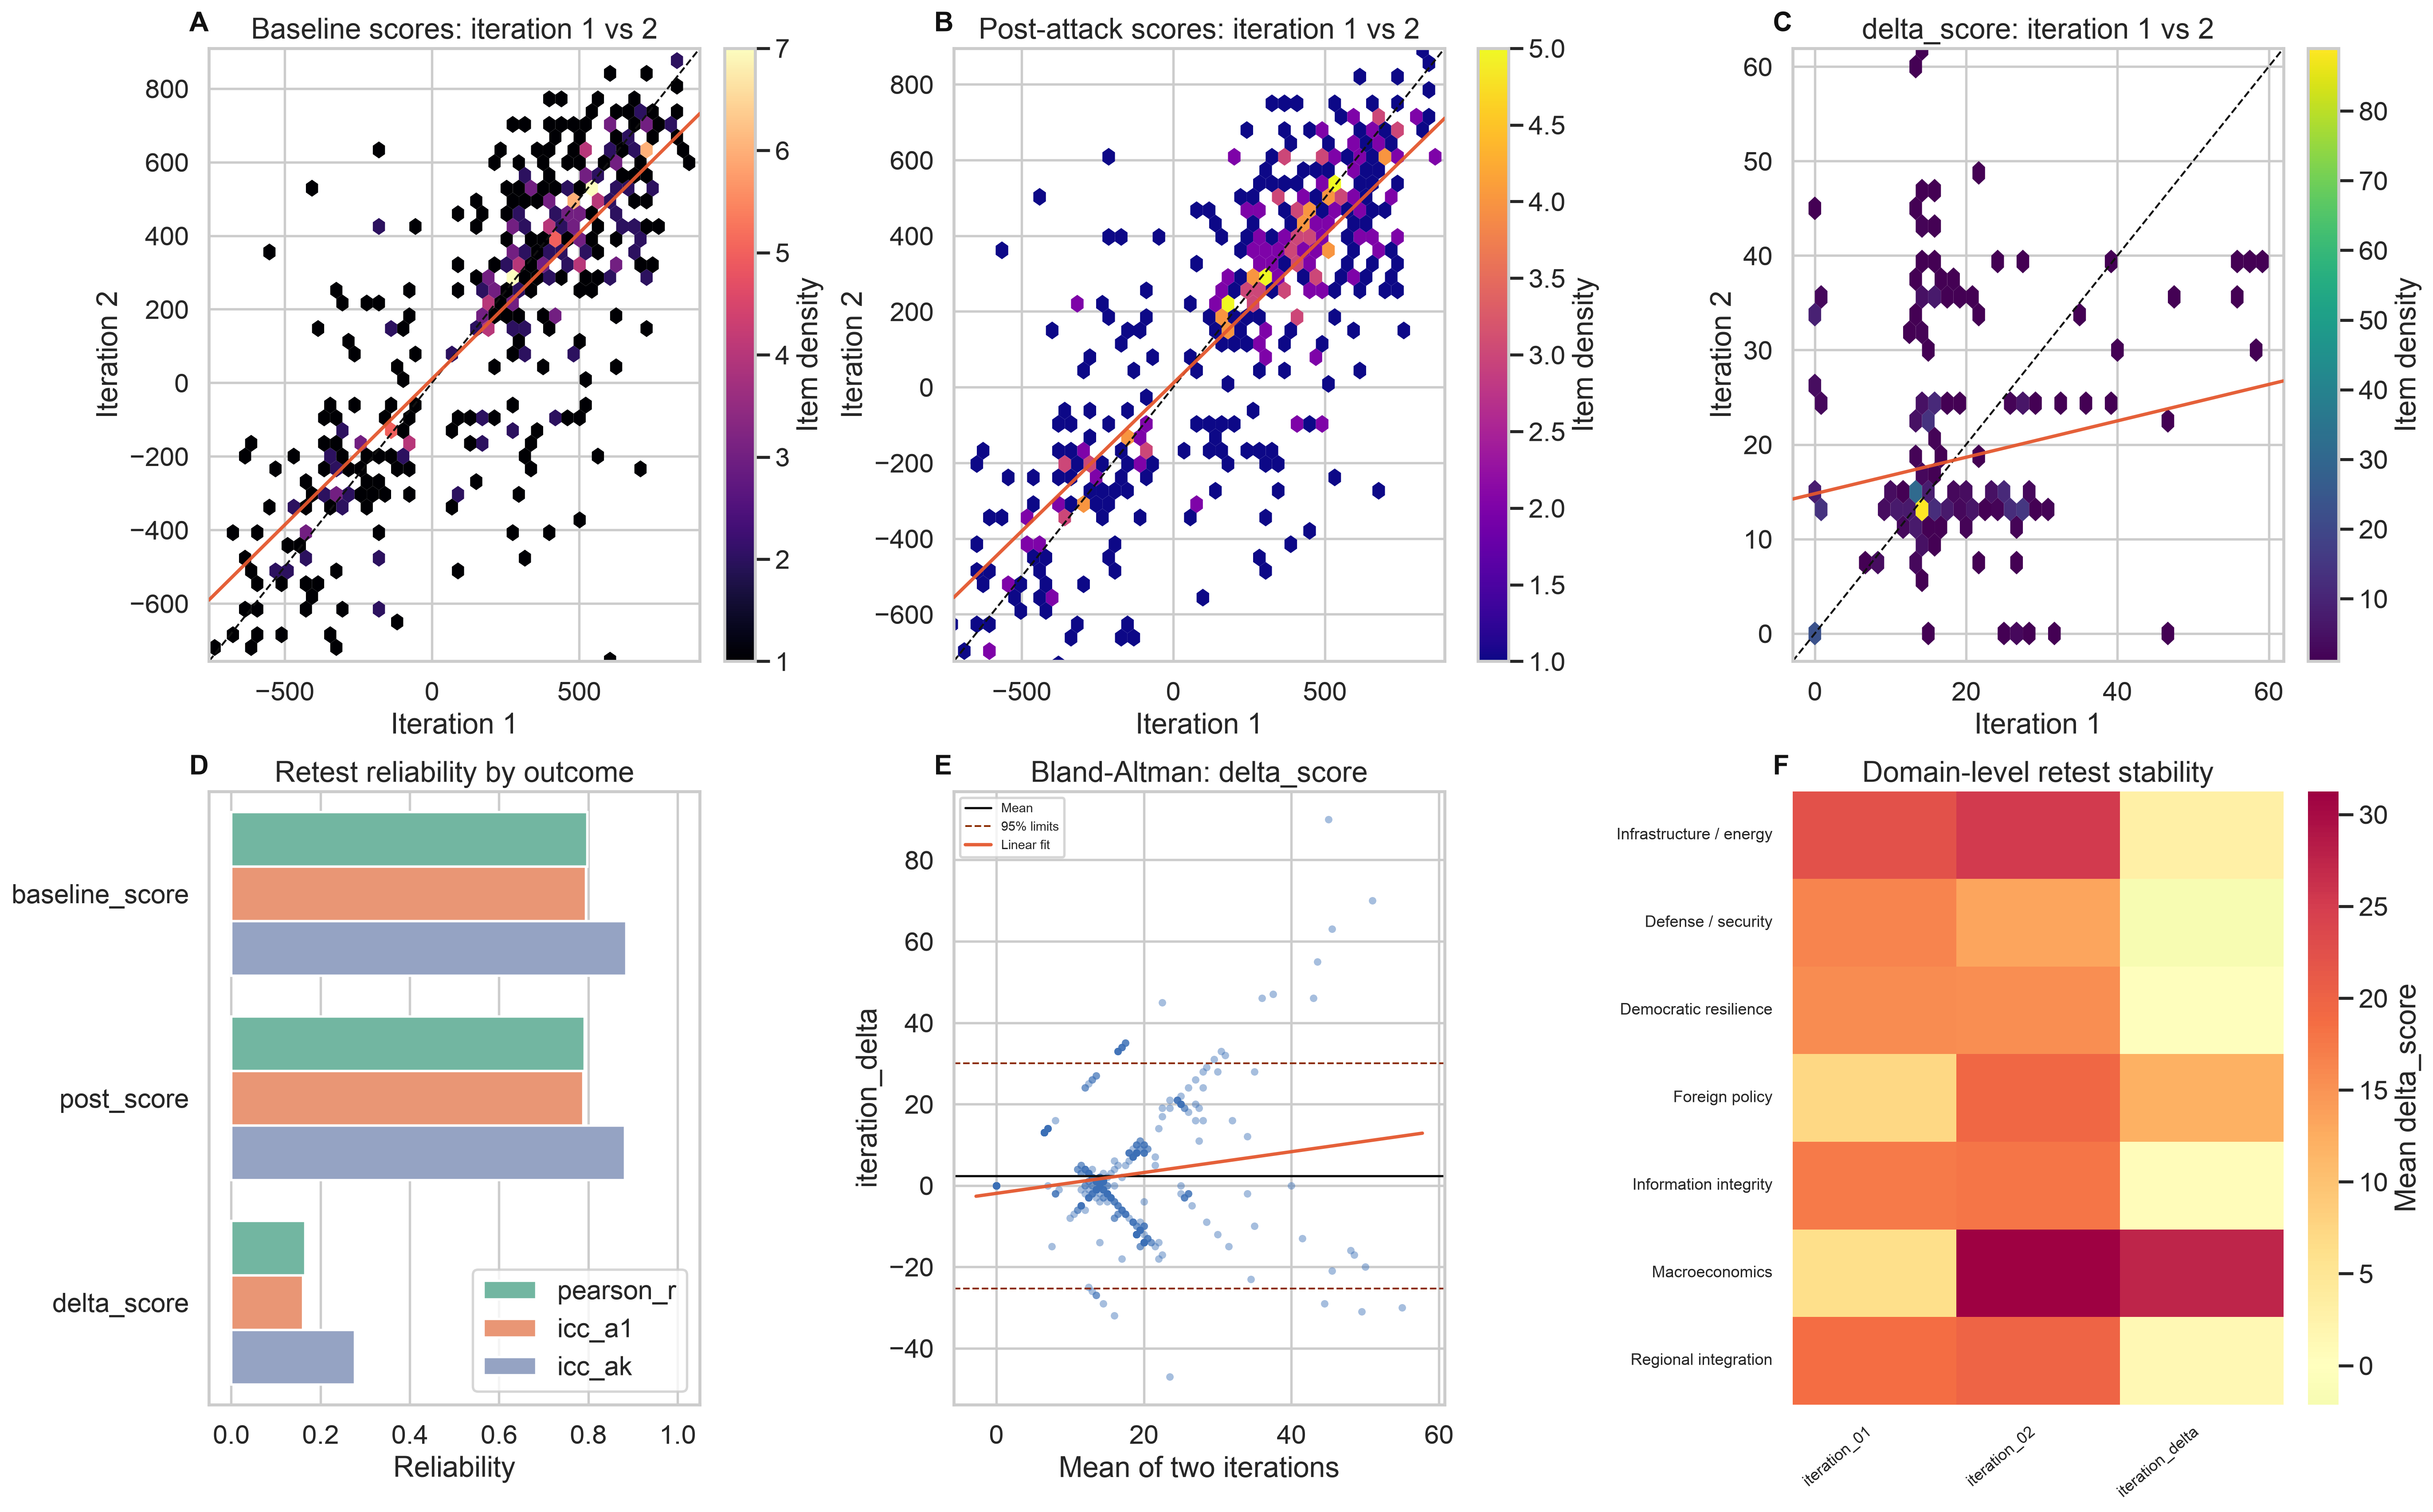
\includegraphics[width=0.9\linewidth]{../assets/figures/sup/SUP1_test_retest_reliability.png}
\apanote{Two identical DeepSeek V4 Flash re-scorings of a fixed subset ($n = 457$ items). (A to
C)~Iteration-1 versus iteration-2 agreement for baseline scores, post-attack scores, and the
per-item delta (hexbin density with identity and linear fit). (D)~Reliability by outcome (Pearson
$r$, ICC(A,1), ICC(A,$k$)). (E)~Bland-Altman plot for the delta. (F)~Domain-level retest stability.
Level scores are reproducible (baseline and post-attack ICC(A,1) $= 0.79$); the delta is noisier
(ICC $= 0.16$).}
\end{figure}

\clearpage

\begin{figure}[H]
\floatleft
\caption{Cross-provider Inter-rater Reliability}
\label{fig:s2}
\vspace{2pt}
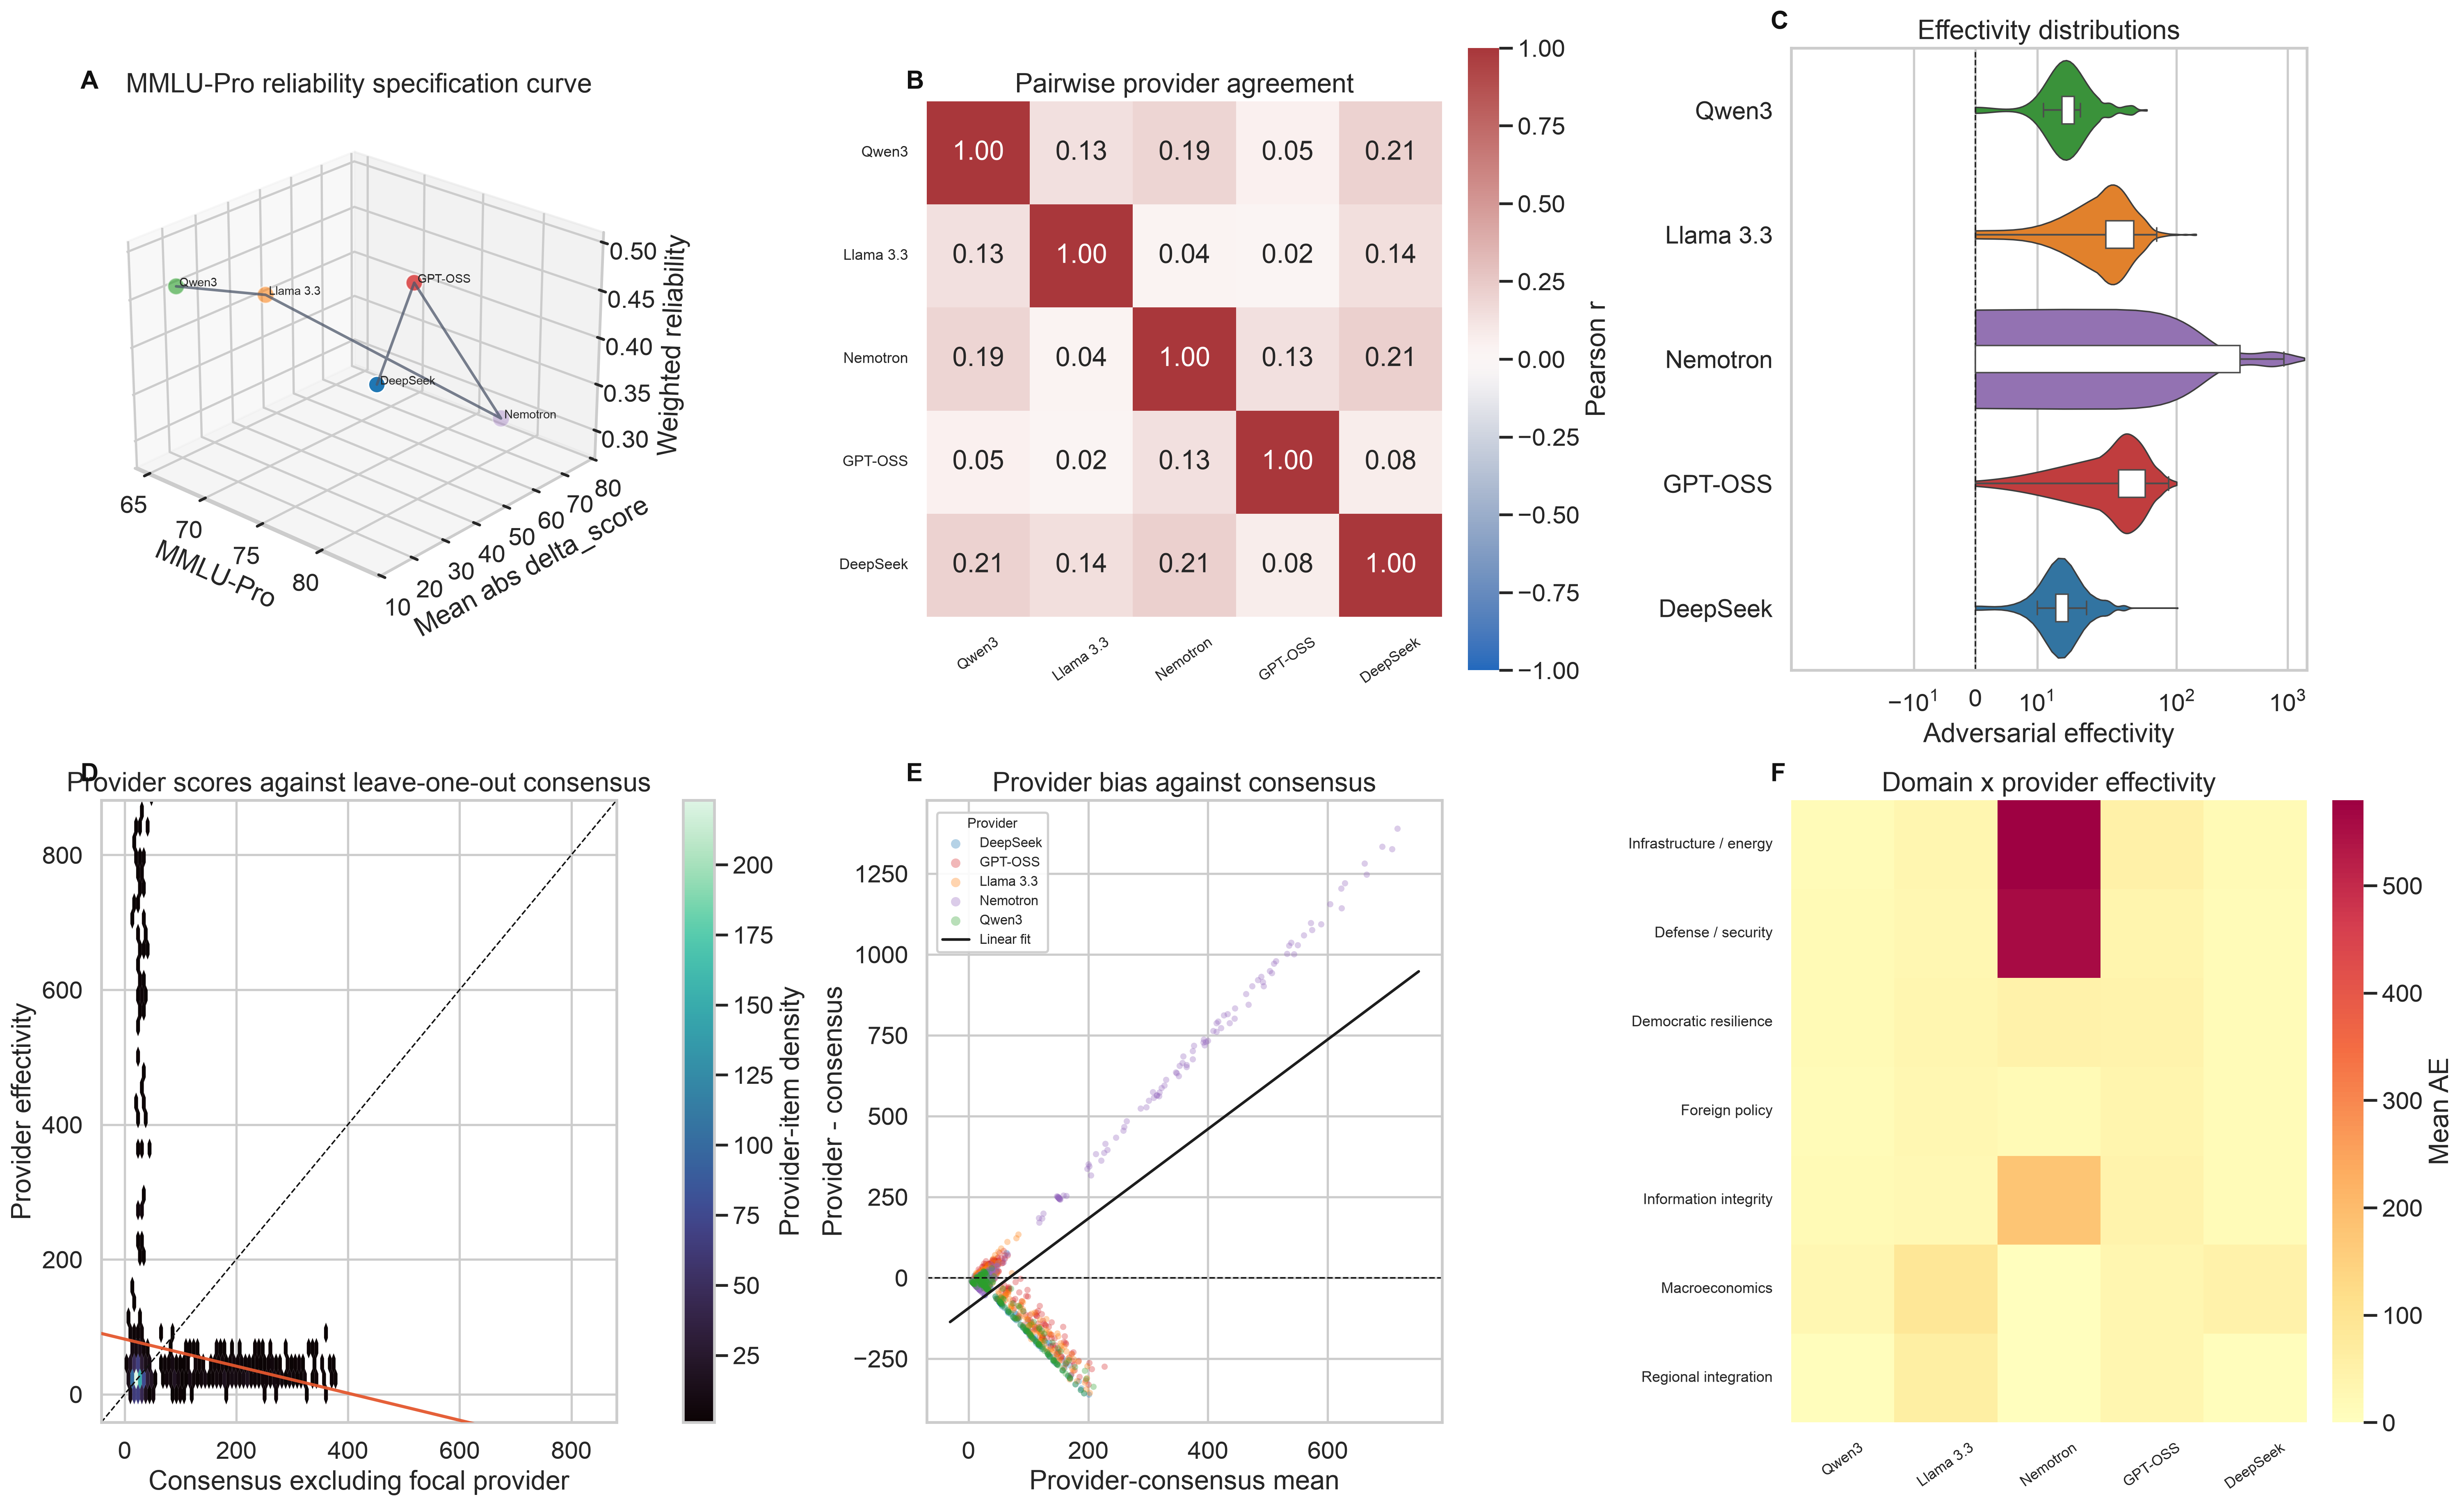
\includegraphics[width=0.9\linewidth]{../assets/figures/sup/SUP2_cross_provider_reliability.png}
\apanote{Five model families (DeepSeek V4 Flash, GPT-OSS 120B, Qwen3 32B, Nemotron 3 Nano 30B,
Llama 3.3 70B) re-score a fixed subset ($n = 311$ items). (A)~Benchmark-versus-reliability
specification curve. (B)~Pairwise provider agreement on effectivity. (C)~Effectivity distributions
by provider. (D)~Provider scores against the leave-one-out consensus. (E)~Provider bias against
consensus. (F)~Domain-by-provider mean effectivity. Opinion levels agree moderately across
providers (baseline ICC $= 0.57$, post-attack $= 0.43$); the raw signed delta agrees weakly (ICC
$= 0.01$).}
\end{figure}

\clearpage

\begin{figure}[H]
\floatleft
\caption{Cross-provider Raw, Percentile, and Rank Reliability Checks}
\label{fig:s3}
\vspace{2pt}
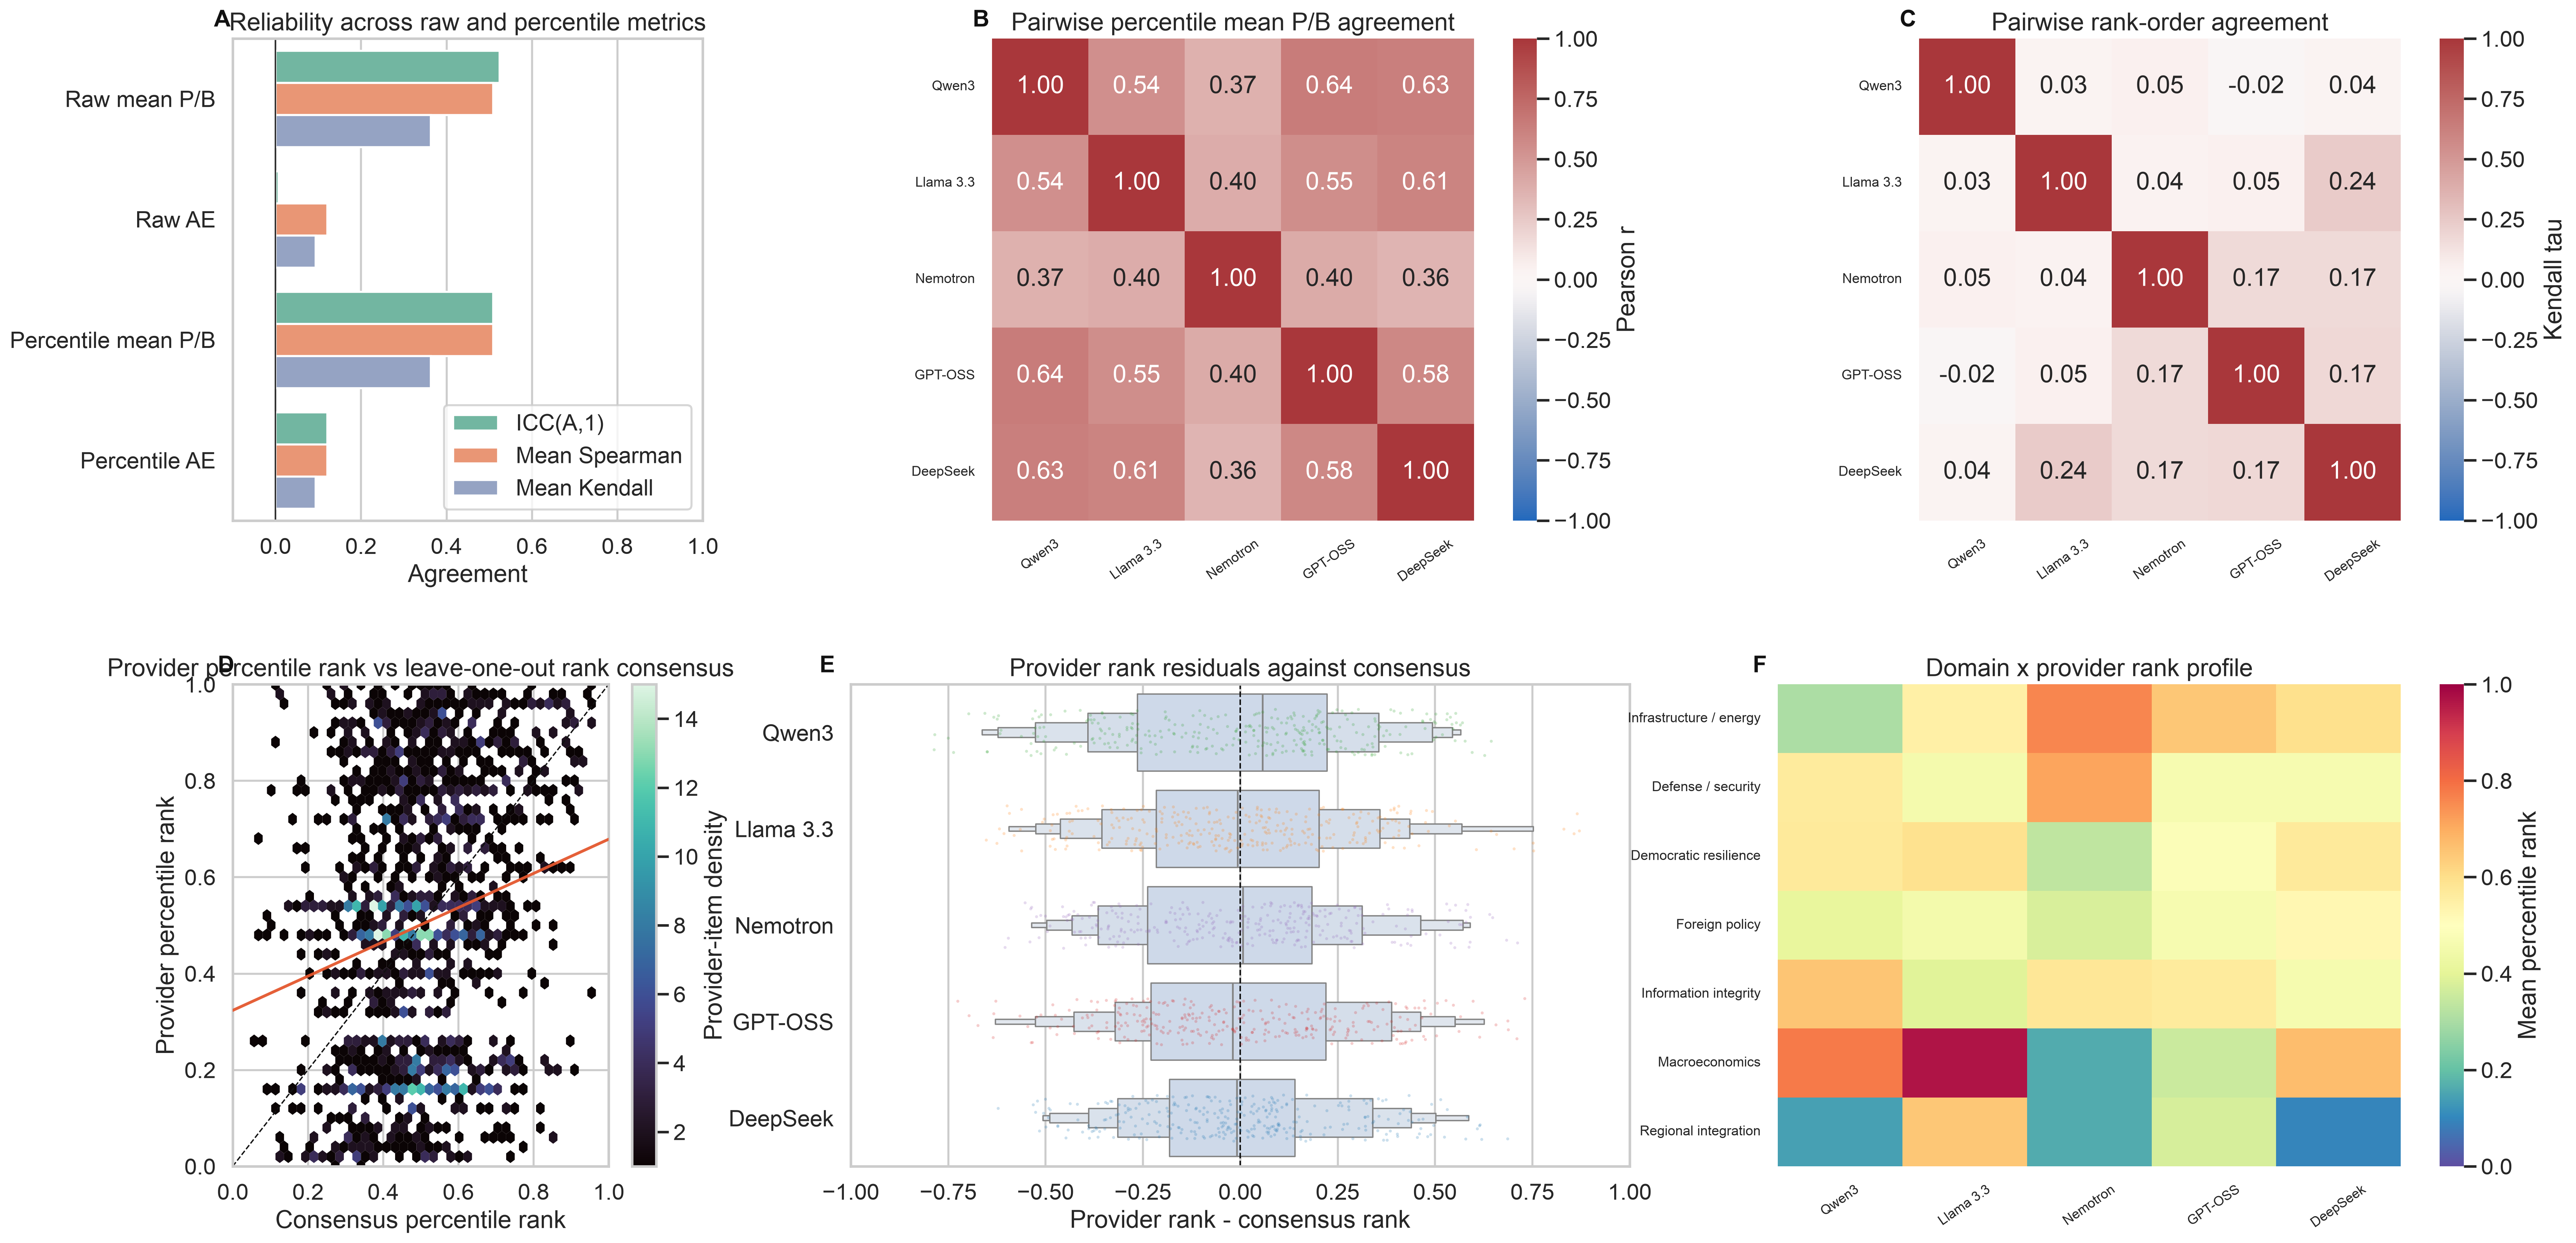
\includegraphics[width=0.9\linewidth]{../assets/figures/sup/SUP3_cross_provider_rank_robustness.png}
\apanote{Robustness of cross-provider agreement under raw, percentile, and rank transforms.
(A)~Reliability across metrics. (B)~Pairwise percentile mean-level agreement. (C)~Pairwise
rank-order agreement on the delta. (D)~Provider percentile rank against the leave-one-out consensus.
(E)~Provider rank residuals. (F)~Domain-by-provider rank profile. Level percentiles are moderately
reproducible (mean pairwise Spearman $= 0.51$); delta percentiles are not (Spearman $= 0.12$).}
\end{figure}

\clearpage

\begin{figure}[H]
\floatleft
\caption{Realized Integrated 10,000-scenario Sampling-design Diagnostics}
\label{fig:s4}
\vspace{2pt}
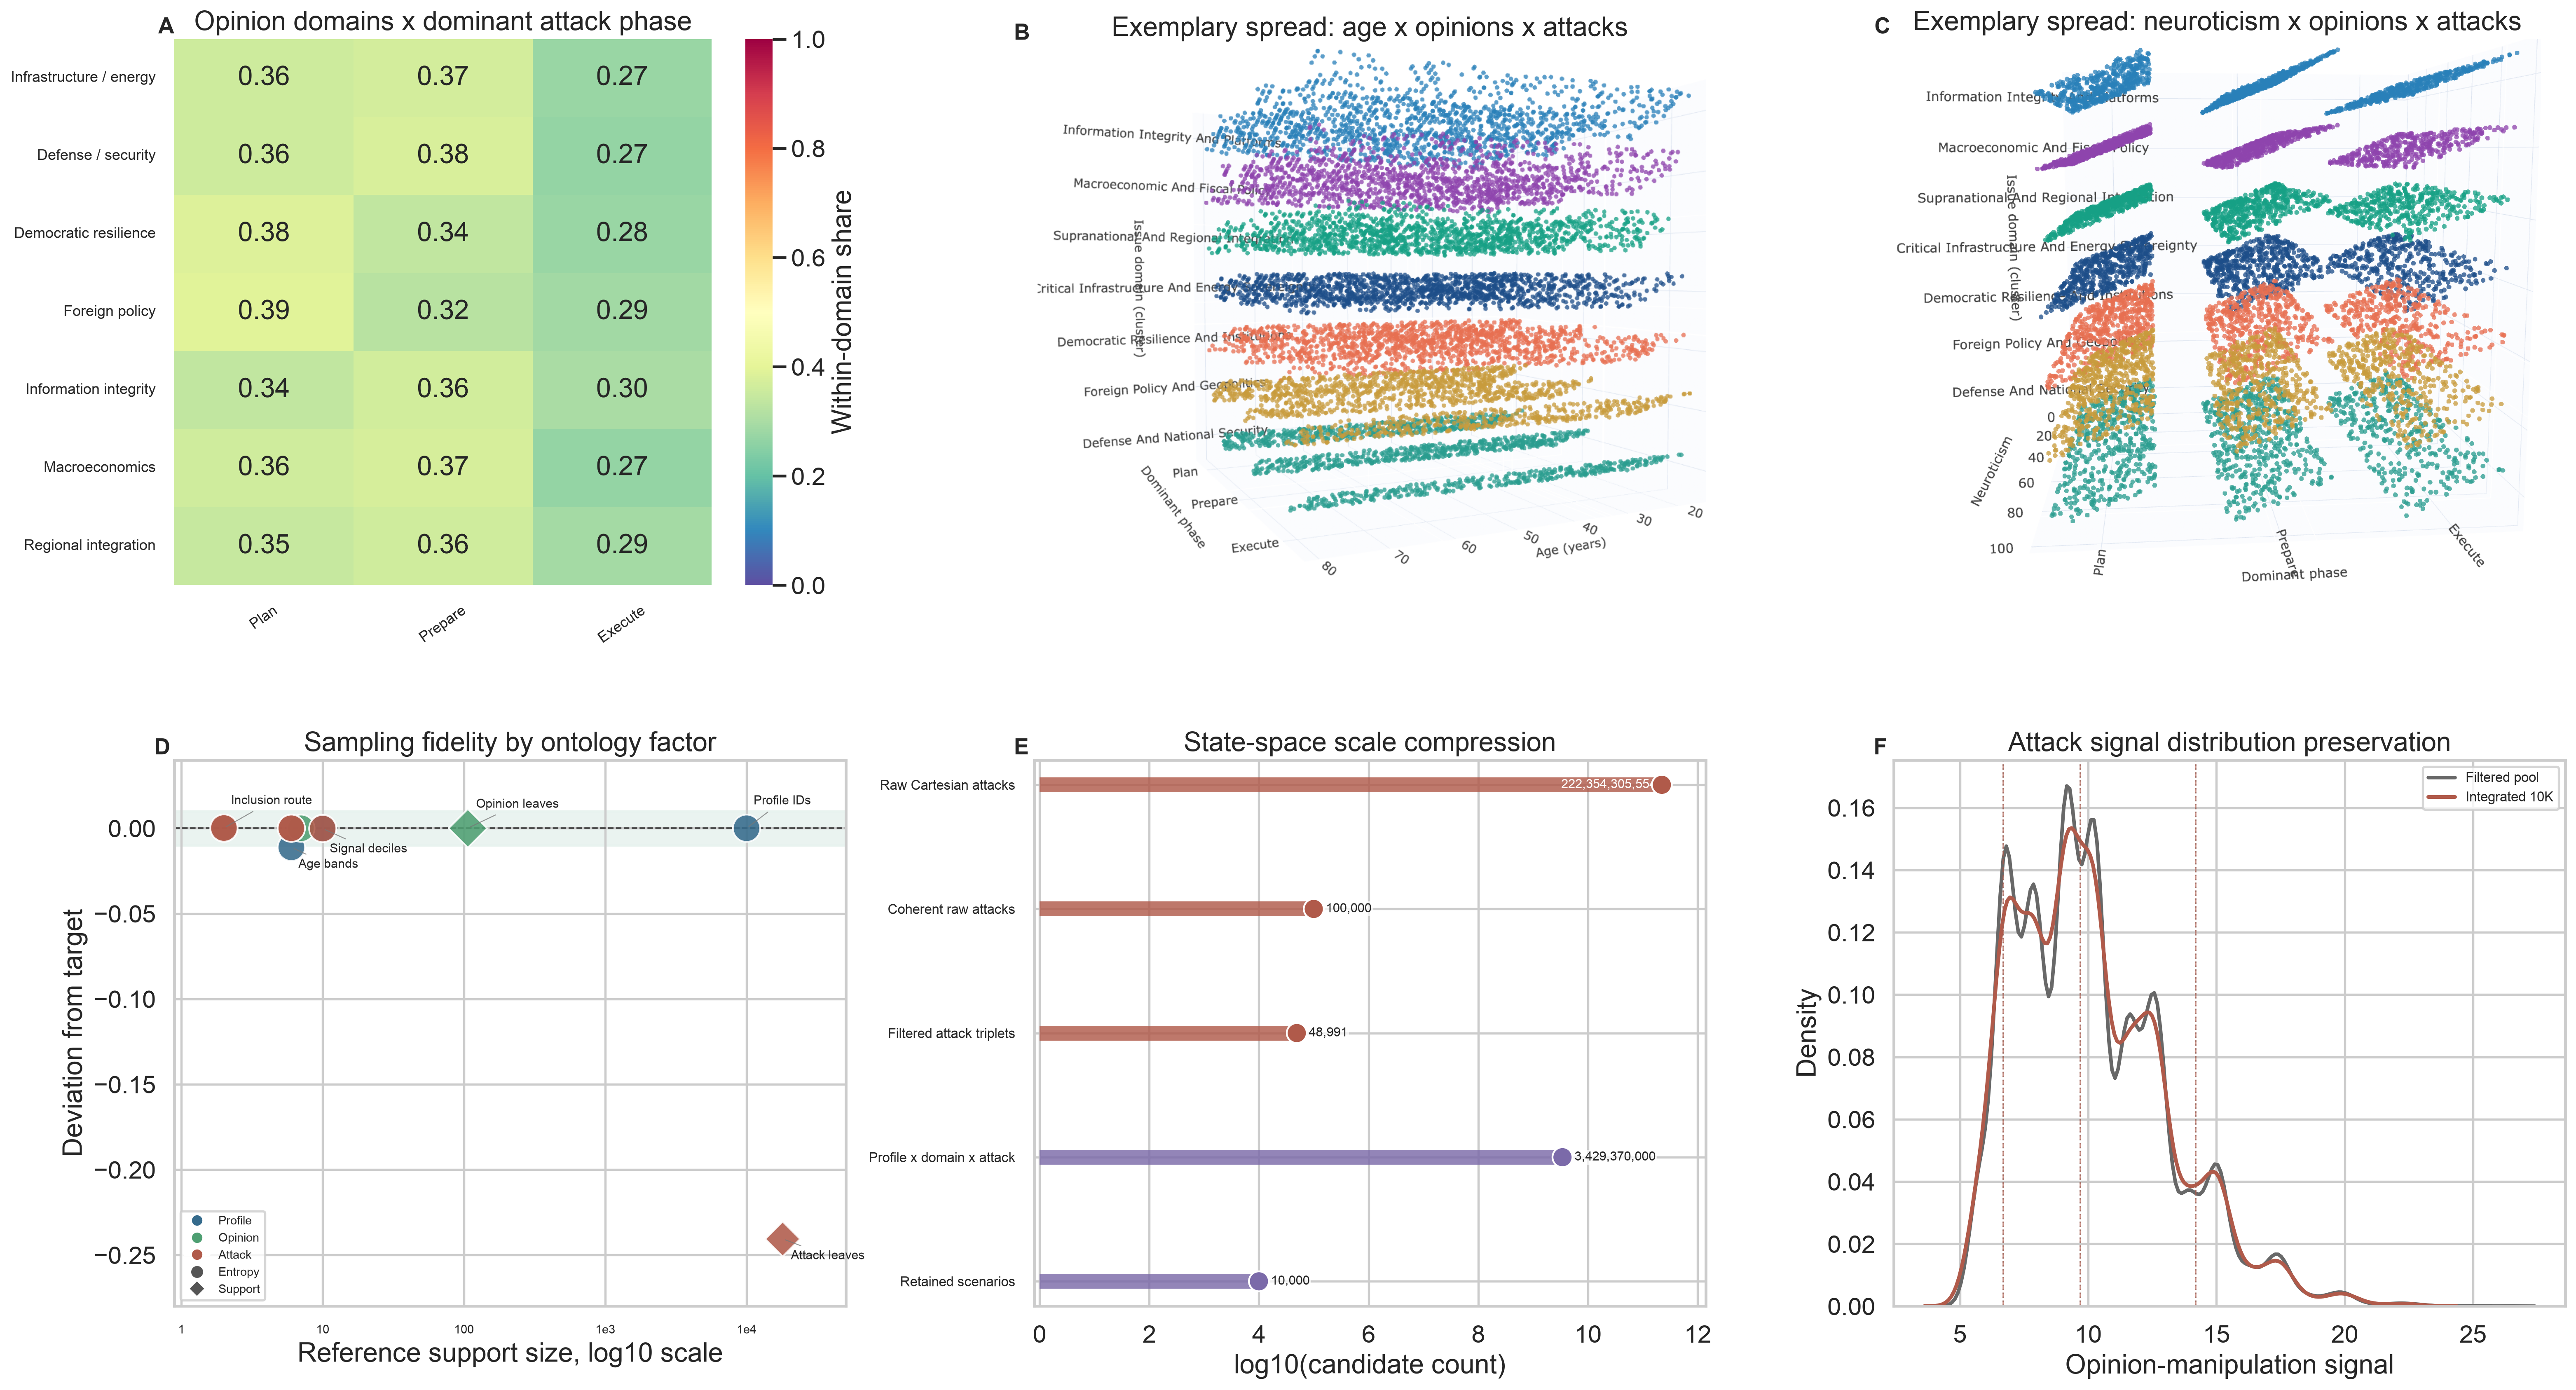
\includegraphics[width=0.95\linewidth]{../assets/figures/sup/SUP4_sampling_design_diagnostics.png}
\apanote{(A)~Within-domain share of the dominant attack phase, confirming attack-phase balance
across opinion domains. (B and C)~Exemplary spread of profile age and neuroticism across opinion
domains and attacks, showing that profile variation is distributed across the design rather than
concentrated. (D)~Sampling fidelity by ontology factor (deviation from the entropy or support
target against reference support size). (E)~Log-scale state-space compression from the raw
candidate spaces into the retained 10,000-scenario design. (F)~Preservation of the attack-signal
distribution relative to the filtered DISARM-red pool. Cross-ontology association is near zero,
supporting independent profile, opinion, and attack assignment.}
\end{figure}

\clearpage

\begin{figure}[H]
\floatleft
\caption{Per-domain Radars of Opinion-leaf Movability}
\label{fig:s5}
\vspace{2pt}
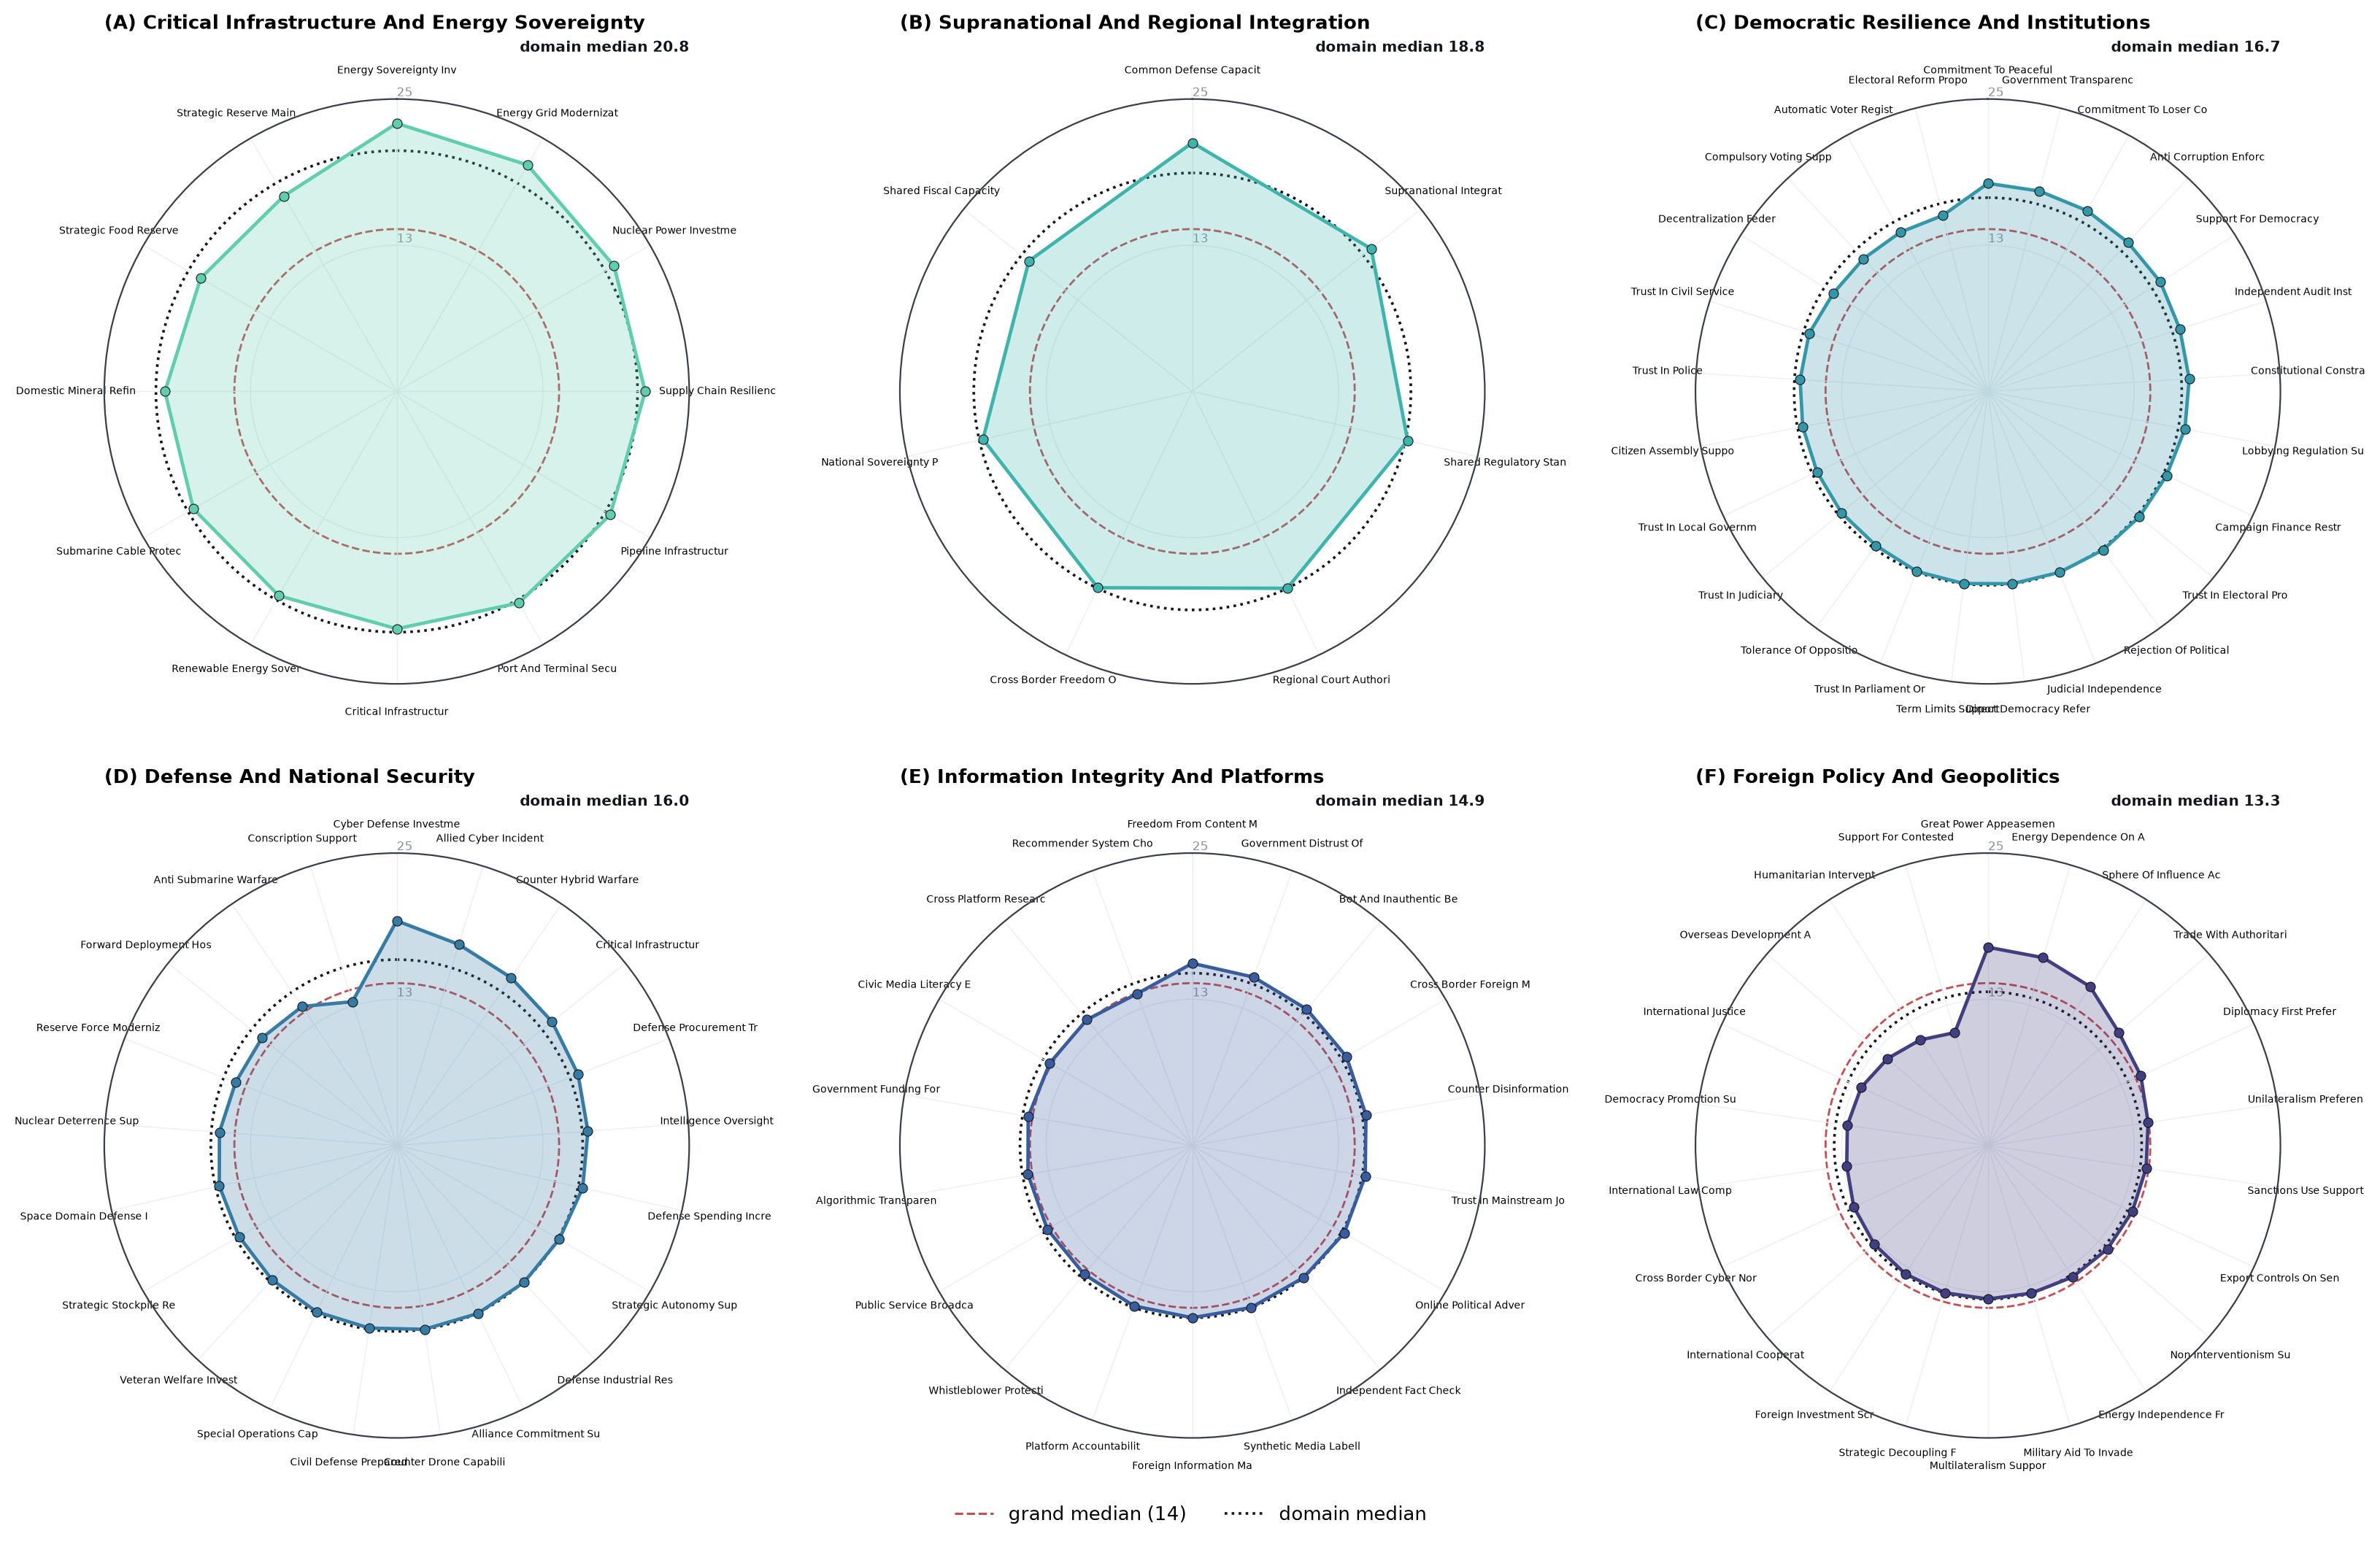
\includegraphics[width=0.95\linewidth]{../assets/figures/sup/SUP5_opinion_polar_hierarchy.png}
\apanote{One radar per issue domain (A to F): the domain's opinion leaves are the spokes and the
radius is each leaf's outlier-clipped mean adversarial effectivity (5th--95th percentile clip),
so the movability fingerprint of each domain's opinion set is legible at a glance. The dashed ring
marks the grand median ($+14$) and the radial scale is shared across panels. The
critical-infrastructure and supranational-integration domains have the widest profiles; information
integrity and defence the tightest.}
\end{figure}

\clearpage

\begin{figure}[H]
\floatleft
\caption{Opinion-cluster Structure With Within-domain Heterogeneity}
\label{fig:s6}
\vspace{2pt}
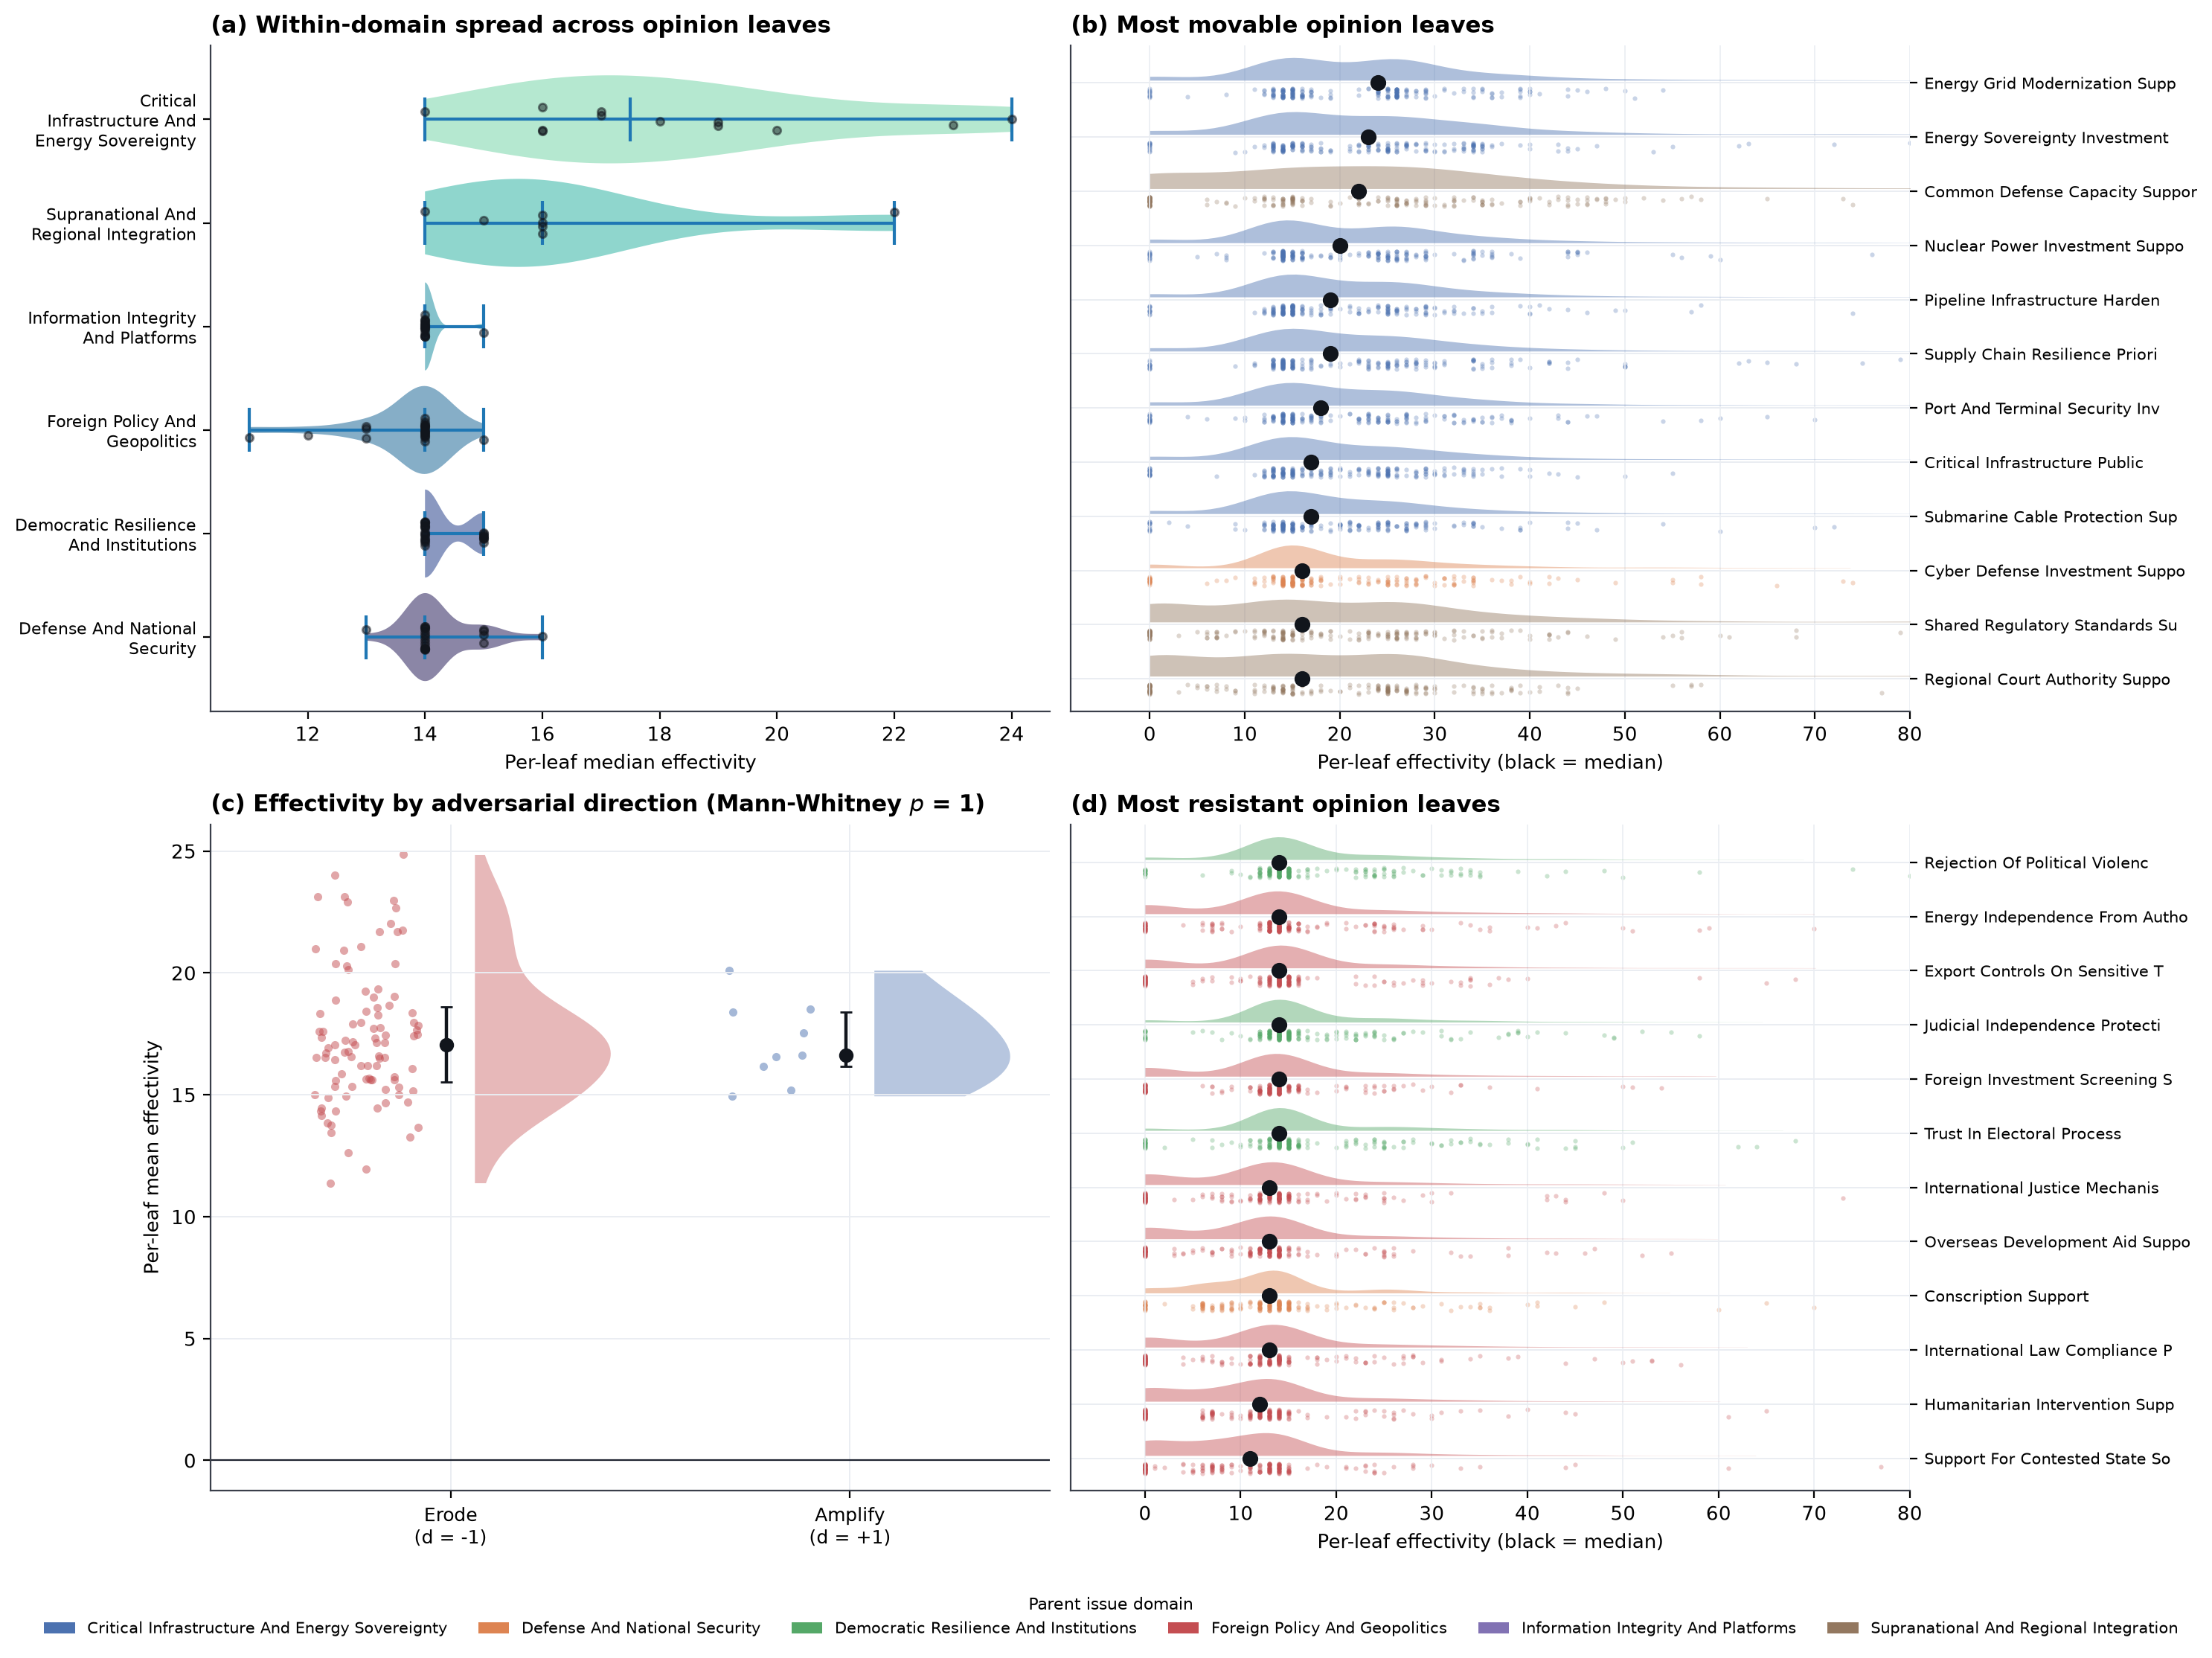
\includegraphics[width=0.94\linewidth]{../assets/figures/sup/SUP6_opinion_clusters.png}
\apanote{(a)~Within-domain spread of per-leaf median effectivity (each domain spans movable and
resistant leaves). (b)~The most movable and (d)~the most resistant individual opinion leaves, each
drawn as a per-leaf raincloud (a half-violin of the leaf's scenario-level effectivity with a black
median dot) coloured by parent issue domain. (c)~Effectivity by adversarial direction: amplify and
erode leaves do not differ (Mann-Whitney $p = 1$), so there is no directional asymmetry once
$d_\ell$ is encoded in the score.}
\end{figure}

\clearpage

\begin{figure}[H]
\floatleft
\caption{Domain-conditional Trait Moderation: Heatmap With Per-domain Radars}
\label{fig:s7}
\vspace{2pt}
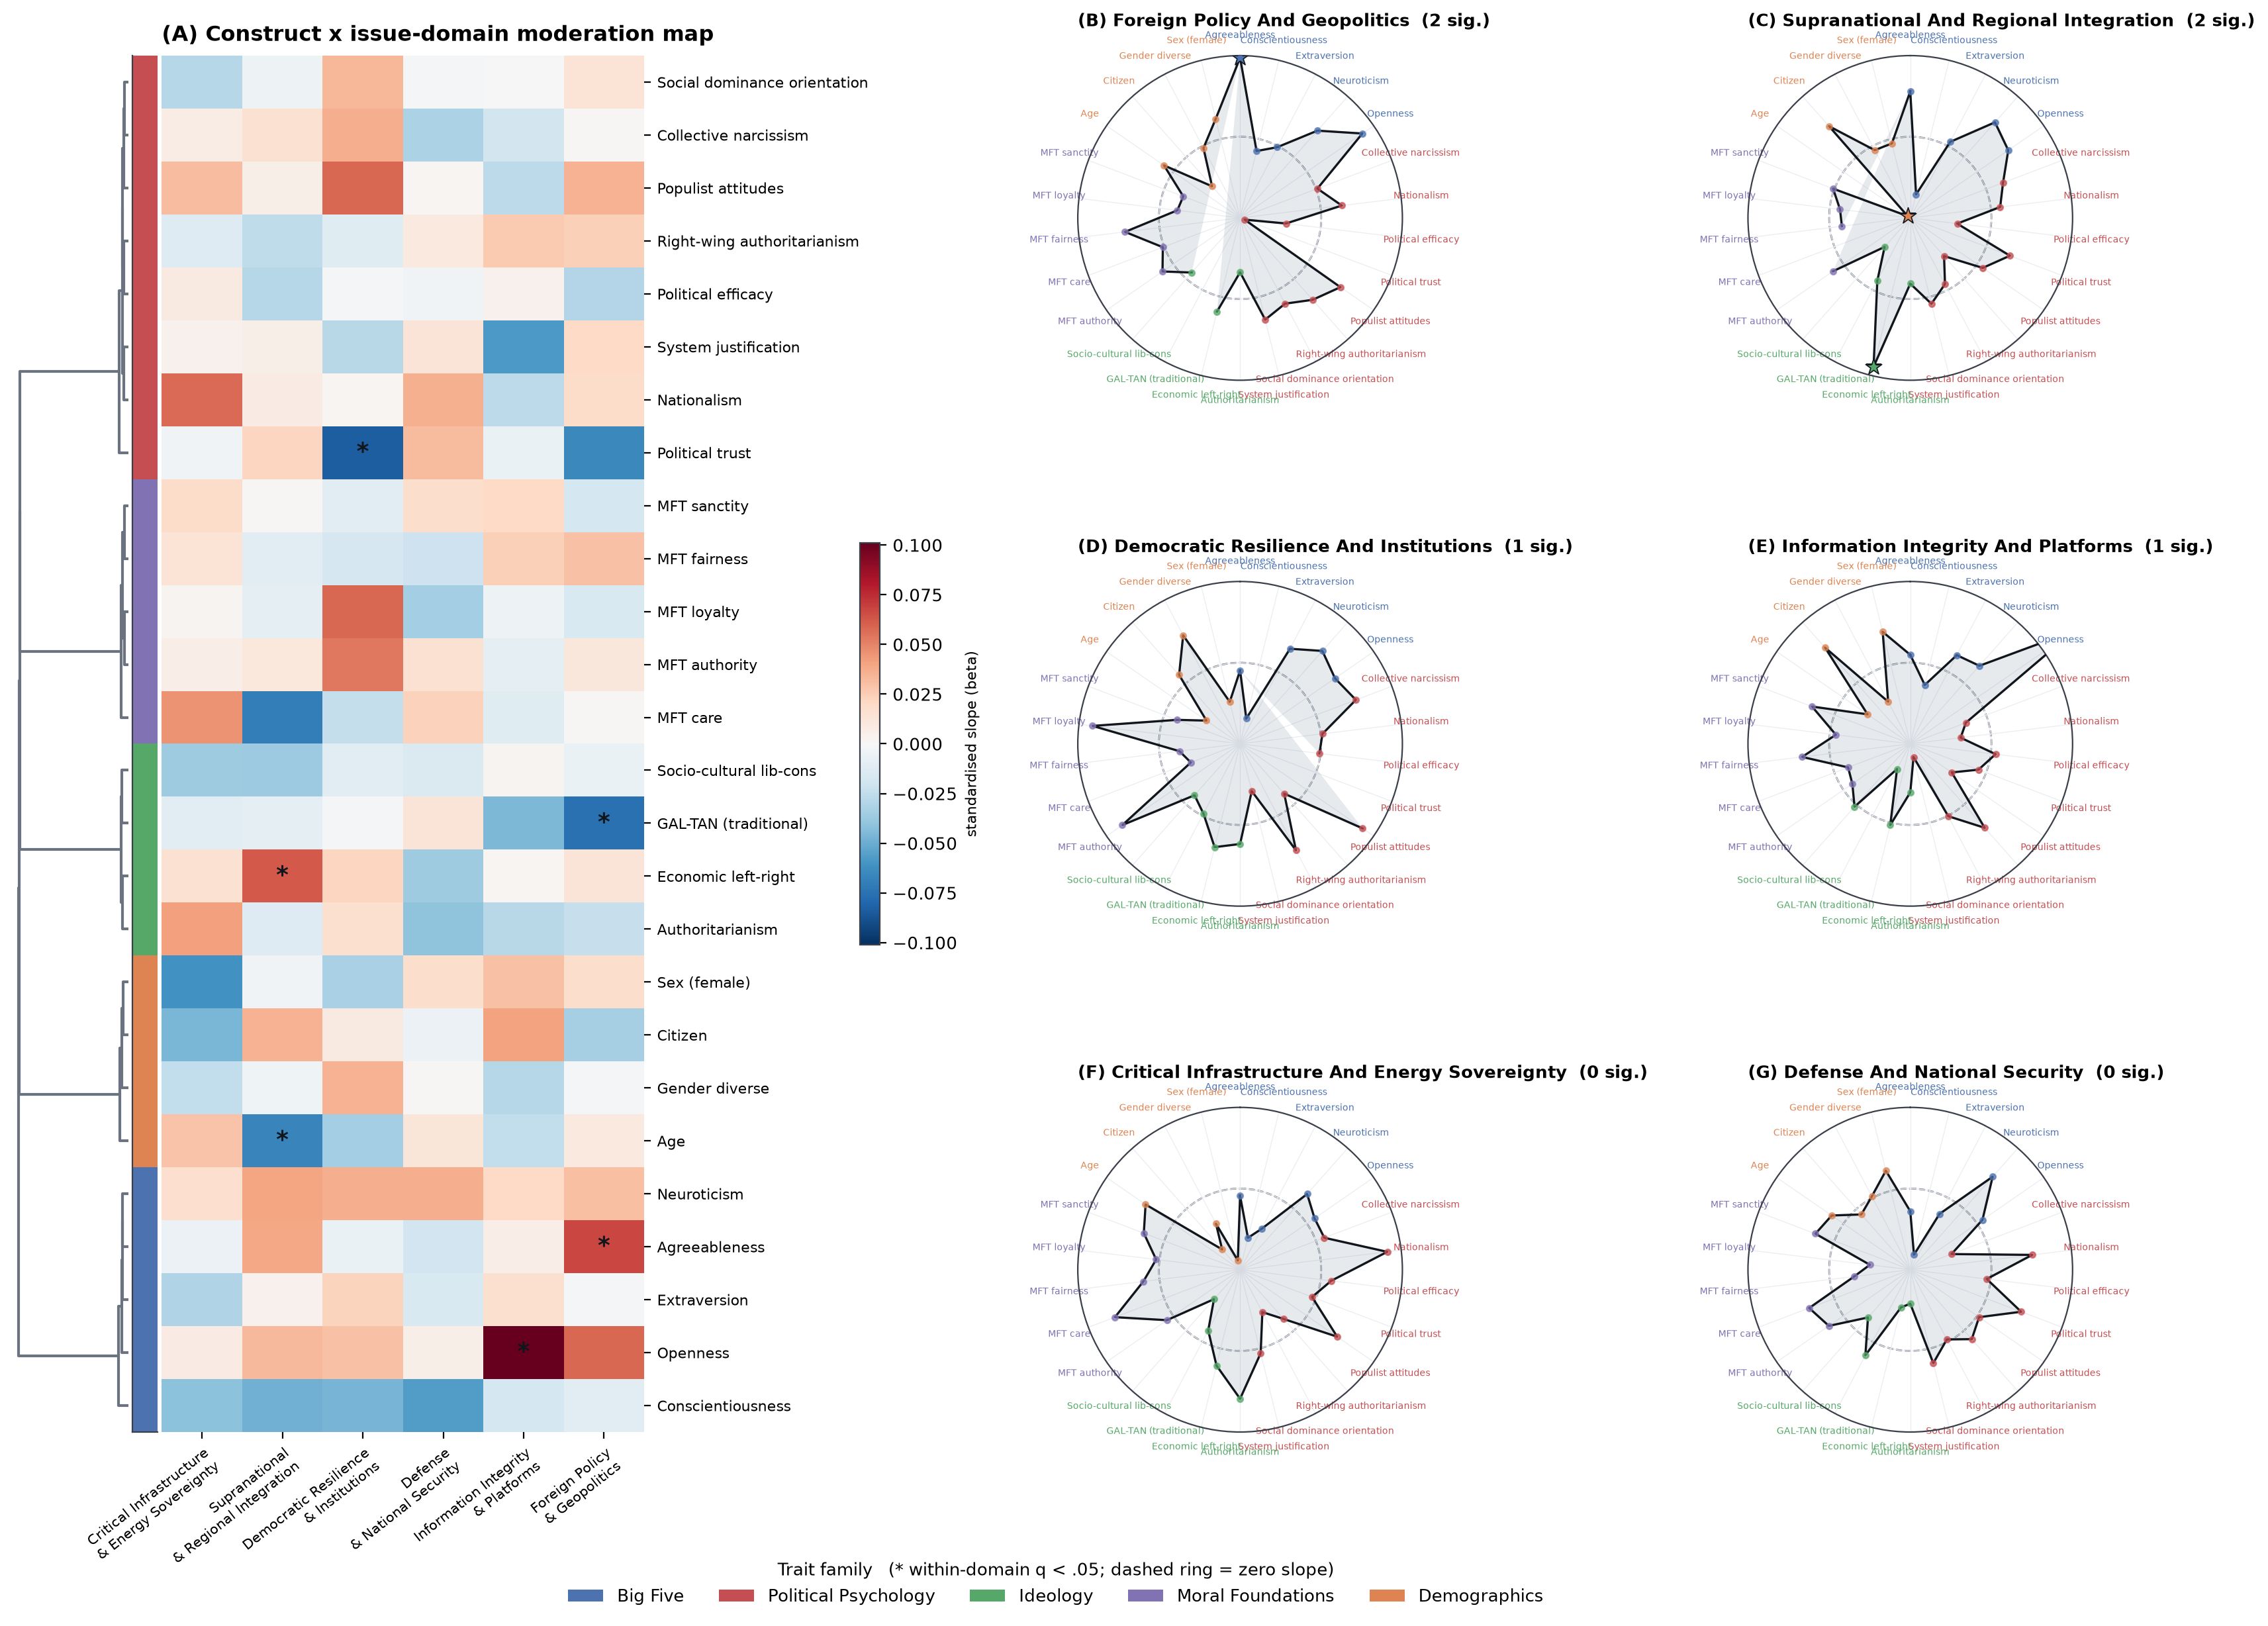
\includegraphics[width=0.99\linewidth]{../assets/figures/sup/SUP7_moderator_by_domain.png}
\apanote{(A)~The full construct-by-domain standardised within-domain moderation-slope heatmap, with
a family-grouped dendrogram on the trait axis and a factor-family colour strip (the dendrogram is
constrained to keep families together); cells significant at Benjamini-Hochberg $q<.05$ are starred
and domains are ordered by movability. (B to G)~One radar per issue domain showing the same
within-domain slopes as a moderation fingerprint, spokes grouped and coloured by family, with
significant constructs starred and a dashed zero-slope reference ring.}
\end{figure}

\clearpage
\suppheading{Supplementary Tables}
\renewcommand{\thetable}{S\arabic{table}}
\setcounter{table}{0}

\begin{table}[H]
\floatleft
\caption{Measurement Reliability by Outcome and Reliability Tier}
\label{tab:s1}
\vspace{2pt}
\begingroup\small
\textit{Panel A. Test-retest, primary model re-scored twice ($n=457$, $k=2$ iterations)}\par\vspace{2pt}
\begin{tabularx}{\linewidth}{@{}Ycccc@{}}
\toprule
Outcome & ICC(A,1) & ICC(A,$k$) & Pearson $r$ & Spearman $\rho$ \\
\midrule
Baseline opinion ($B$) & 0.79 & 0.89 & 0.80 & 0.77 \\
Post-attack opinion ($P$) & 0.79 & 0.88 & 0.79 & 0.77 \\
Signed delta ($P-B$) & 0.53 & 0.70 & 0.55 & 0.38 \\
Effectivity ($\mathrm{AE}$) & 0.16 & 0.28 & 0.17 & 0.17 \\
\bottomrule
\end{tabularx}

\vspace{6pt}
\textit{Panel B. Cross-provider, five independent model families ($n=311$, $k=5$ raters)}\par\vspace{2pt}
\begin{tabularx}{\linewidth}{@{}Yccc@{}}
\toprule
Outcome & ICC(A,1) & ICC(A,$k$) & Mean pairwise Spearman $\rho$ \\
\midrule
Baseline opinion ($B$) & 0.57 & 0.87 & 0.52 \\
Post-attack opinion ($P$) & 0.43 & 0.79 & 0.46 \\
Signed delta ($P-B$) & 0.03 & 0.13 & --- \\
Effectivity ($\mathrm{AE}$) & 0.01 & 0.03 & 0.12 \\
\bottomrule
\end{tabularx}
\endgroup
\apanote{Absolute-agreement intraclass correlations; ICC(A,1) is the reliability of a single
rater and ICC(A,$k$) that of the $k$-rater mean. The five cross-provider families are DeepSeek
V4 Flash, GPT-OSS 120B, Qwen3 32B, Nemotron 3 Nano 30B, and Llama 3.3 70B. Opinion levels are
reproducible and aggregate well across raters, whereas the direction-adjusted effectivity is
intrinsically noisier because a difference score amplifies level noise. Under a percentile
(rank) transform the cross-provider level agreement recovers to a mean pairwise Spearman of
0.51, while the delta percentile remains at 0.12, so aggregate and direction-level findings are
emphasised over fine-grained per-scenario delta magnitudes.}
\end{table}

\clearpage

\begin{table}[H]
\floatleft
\caption{Issue-domain Susceptibility Summary}
\label{tab:domains}
\vspace{2pt}
\begingroup\footnotesize
\begin{tabularx}{\linewidth}{@{}Y*{7}{c}@{}}
\toprule
Issue domain & Leaves & $n$ & Mdn & Mean & IQR (Q1, Q3) & \% toward goal & $|r_{\mathrm{rb}}|$ vs ref \\
\midrule
Critical Infrastructure and Energy Sovereignty & 12 & 1{,}429 & 19.0 & 22.5 & (14.3, 26.2) & 94.4 & 0.46 \\
Supranational and Regional Integration & 7 & 1{,}428 & 16.8 & 20.6 & (7.3, 27.4) & 81.2 & 0.22 \\
Democratic Resilience and Institutions & 25 & 1{,}429 & 14.3 & 17.7 & (13.5, 19.6) & 94.6 & 0.25 \\
Defense and National Security & 21 & 1{,}429 & 14.3 & 16.9 & (12.8, 19.0) & 92.5 & 0.20 \\
Information Integrity and Platforms & 18 & 1{,}428 & 14.0 & 15.7 & (13.1, 15.2) & 90.0 & 0.14 \\
Foreign Policy and Geopolitics & 22 & 1{,}429 & 13.5 & 14.7 & (10.1, 16.6) & 81.2 & ref \\
\bottomrule
\end{tabularx}
\endgroup
\apanote{Scenario-level adversarial effectivity on the 2,001-position scale, computed on the
independent scenario means after excluding the single-leaf macroeconomic domain. Columns:
number of directional opinion leaves, analysed scenarios, median (Mdn) and mean effectivity,
the interquartile range, the share of scenarios moving toward the attacker goal, and the
absolute rank-biserial effect of the scenario-level Mann-Whitney contrast against the
least-movable reference domain (foreign policy). Omnibus Kruskal-Wallis $H = 579.1$,
$p = 6.8\mathrm{e}{-123}$, $\varepsilon^2 = 0.067$.}
\end{table}

\clearpage

\begin{table}[H]
\floatleft
\caption{Pairwise Issue-domain Contrasts (Absolute Rank-biserial Effect)}
\label{tab:dompairs}
\vspace{2pt}
\begingroup\small
\begin{tabularx}{\linewidth}{@{}Xccccc@{}}
\toprule
 & SR & DR & DN & II & FP \\
\midrule
CI (most movable) & 0.11 & 0.30 & 0.33 & 0.41 & 0.46 \\
SR & & 0.07 & 0.10 & 0.16 & 0.22 \\
DR & & & 0.05 & 0.14 & 0.25 \\
DN & & & & 0.09 & 0.20 \\
II & & & & & 0.14 \\
\bottomrule
\end{tabularx}
\endgroup
\apanote{Absolute rank-biserial effect size for every pairwise scenario-level Mann-Whitney
contrast, ordered by movability. Domain codes: CI~=~Critical Infrastructure and Energy
Sovereignty, SR~=~Supranational and Regional Integration, DR~=~Democratic Resilience and
Institutions, DN~=~Defense and National Security, II~=~Information Integrity and Platforms,
FP~=~Foreign Policy and Geopolitics. All fifteen contrasts are significant after
Benjamini-Hochberg correction ($q<.05$); magnitude rises with separation in movability, and the
extreme CI-versus-FP contrast reaches 0.46.}
\end{table}

\clearpage

\begin{table}[H]
\floatleft
\caption{Full Cross-family Curated Moderator Model}
\label{tab:curatedfull}
\vspace{2pt}
\begingroup\small
\begin{tabularx}{\linewidth}{@{}Yp{2.1cm}ccc@{}}
\toprule
Moderator & Family & $\beta_{\text{std}}$ & 95\% CI & $q$ \\
\midrule
\textbf{Openness} & Big Five & $\mathbf{+0.042}$ & $[+0.020, +0.063]$ & \textbf{.004} \\
\textbf{Conscientiousness} & Big Five & $\mathbf{-0.035}$ & $[-0.055, -0.014]$ & \textbf{.013} \\
\textbf{Neuroticism} & Big Five & $\mathbf{+0.030}$ & $[+0.009, +0.050]$ & \textbf{.045} \\
Socio-cultural lib-cons & Ideology & $-0.022$ & $[-0.043, +0.000]$ & .323 \\
GAL-TAN (traditional) & Ideology & $-0.018$ & $[-0.039, +0.004]$ & .451 \\
Populist attitudes & Pol.\ psych. & $+0.017$ & $[-0.005, +0.039]$ & .451 \\
Agreeableness & Big Five & $+0.016$ & $[-0.005, +0.037]$ & .451 \\
Economic left-right & Ideology & $+0.015$ & $[-0.006, +0.036]$ & .451 \\
MFT authority & Moral Found. & $+0.015$ & $[-0.006, +0.035]$ & .451 \\
Nationalism & Pol.\ psych. & $+0.015$ & $[-0.007, +0.036]$ & .451 \\
Age & Demographics & $-0.014$ & $[-0.035, +0.007]$ & .451 \\
Political efficacy & Pol.\ psych. & $-0.012$ & $[-0.033, +0.009]$ & .563 \\
Political trust & Pol.\ psych. & $-0.010$ & $[-0.032, +0.012]$ & .713 \\
Sex (female) & Demographics & $-0.008$ & $[-0.029, +0.013]$ & .820 \\
MFT care & Moral Found. & $-0.008$ & $[-0.029, +0.013]$ & .820 \\
Collective narcissism & Pol.\ psych. & $+0.007$ & $[-0.014, +0.028]$ & .820 \\
Authoritarianism & Ideology & $-0.006$ & $[-0.027, +0.015]$ & .855 \\
Citizen & Demographics & $-0.004$ & $[-0.026, +0.017]$ & .912 \\
System justification & Pol.\ psych. & $-0.004$ & $[-0.025, +0.017]$ & .912 \\
Social dominance orientation & Pol.\ psych. & $-0.004$ & $[-0.025, +0.017]$ & .912 \\
Extraversion & Big Five & $-0.004$ & $[-0.025, +0.018]$ & .912 \\
MFT sanctity & Moral Found. & $+0.003$ & $[-0.018, +0.024]$ & .912 \\
MFT fairness & Moral Found. & $+0.003$ & $[-0.019, +0.024]$ & .912 \\
Gender diverse & Demographics & $+0.002$ & $[-0.019, +0.023]$ & .944 \\
Right-wing authoritarianism & Pol.\ psych. & $-0.001$ & $[-0.021, +0.020]$ & .982 \\
MFT loyalty & Moral Found. & $-0.000$ & $[-0.021, +0.021]$ & .998 \\
\bottomrule
\end{tabularx}
\endgroup
\apanote{All 26 curated constructs (one interpretable score per construct) entered jointly in a
single cross-family ordinary-least-squares model with HC3 robust standard errors ($n = 8{,}572$
scenarios, model $R^2 = 0.007$). Standardised slopes with 95\% confidence intervals, ranked by
absolute slope; $q$ values are Benjamini-Hochberg corrected across the model. Boldface marks the
three constructs surviving $q<.05$, all from the Big Five. Positive slopes indicate greater
movability.}
\end{table}

\clearpage

\begin{table}[H]
\floatleft
\caption{Big Five Facet-level Moderators Significant Within Family}
\label{tab:facets}
\vspace{2pt}
\begingroup\small
\begin{tabularx}{\linewidth}{@{}Yccc@{}}
\toprule
Construct (domain score and facets) & $\beta_{\text{std}}$ & 95\% CI & $q$ \\
\midrule
\textbf{Openness to Experience} & $+0.040$ & $[+0.019, +0.062]$ & .002 \\
\quad Values & $+0.041$ & $[+0.019, +0.063]$ & .002 \\
\quad Feelings & $+0.039$ & $[+0.018, +0.060]$ & .002 \\
\quad Aesthetics & $+0.037$ & $[+0.015, +0.058]$ & .004 \\
\quad Ideas & $+0.037$ & $[+0.015, +0.058]$ & .004 \\
\quad Fantasy & $+0.036$ & $[+0.014, +0.058]$ & .004 \\
\quad Actions & $+0.033$ & $[+0.012, +0.054]$ & .007 \\
\addlinespace
\textbf{Conscientiousness} & $-0.035$ & $[-0.056, -0.014]$ & .004 \\
\quad Self-Discipline & $-0.039$ & $[-0.060, -0.019]$ & .002 \\
\quad Achievement-Striving & $-0.036$ & $[-0.056, -0.015]$ & .004 \\
\quad Competence & $-0.032$ & $[-0.052, -0.011]$ & .009 \\
\quad Deliberation & $-0.030$ & $[-0.051, -0.010]$ & .011 \\
\quad Order & $-0.030$ & $[-0.051, -0.009]$ & .011 \\
\quad Dutifulness & $-0.027$ & $[-0.048, -0.006]$ & .024 \\
\addlinespace
\textbf{Neuroticism} & $+0.030$ & $[+0.009, +0.050]$ & .011 \\
\quad Impulsiveness & $+0.031$ & $[+0.010, +0.052]$ & .011 \\
\quad Anger / Hostility & $+0.028$ & $[+0.008, +0.049]$ & .016 \\
\quad Stress Vulnerability & $+0.027$ & $[+0.005, +0.048]$ & .026 \\
\quad Anxiety & $+0.025$ & $[+0.005, +0.046]$ & .030 \\
\quad Self-Consciousness & $+0.025$ & $[+0.004, +0.045]$ & .031 \\
\quad Depression & $+0.024$ & $[+0.003, +0.045]$ & .047 \\
\bottomrule
\end{tabularx}
\endgroup
\apanote{Standardised univariate slopes (HC3 robust standard errors, $n = 8{,}572$) for the Big
Five constructs and their facets that survive Benjamini-Hochberg correction within the Big Five
family. No facet of the political-psychology, ideology, moral-foundations, or demographic
families reached within-family significance. The facet structure shows that the three
domain-level effects are broad rather than driven by a single narrow facet: openness and its
intellect-oriented facets predict greater movability, conscientiousness and its
self-regulation facets predict resistance, and neuroticism and its negative-affect facets
predict greater movability.}
\end{table}

\clearpage

\begin{table}[H]
\floatleft
\caption{Significant Domain-conditional Trait Moderators}
\label{tab:bydomain}
\vspace{2pt}
\begingroup\small
\begin{tabularx}{\linewidth}{@{}Yp{3.0cm}cp{2.4cm}cc@{}}
\toprule
Issue domain & Moderator (family) & $\beta_{\text{std}}$ & 95\% CI & $p$ & $q$ \\
\midrule
Information Integrity and Platforms & Openness (Big Five) & $+0.101$ & $[+0.041, +0.161]$ & .001 & .005 \\
Democratic Resilience and Institutions & Political trust (Pol.\ psych.) & $-0.083$ & $[-0.137, -0.029]$ & .002 & .020 \\
Foreign Policy and Geopolitics & GAL-TAN, traditional (Ideology) & $-0.075$ & $[-0.130, -0.020]$ & .008 & .030 \\
Foreign Policy and Geopolitics & Agreeableness (Big Five) & $+0.068$ & $[+0.019, +0.116]$ & .006 & .031 \\
Supranational and Regional Integration & Age (Demographics) & $-0.067$ & $[-0.117, -0.017]$ & .009 & .009 \\
Supranational and Regional Integration & Economic left-right (Ideology) & $+0.062$ & $[+0.014, +0.110]$ & .012 & .047 \\
\bottomrule
\end{tabularx}
\endgroup
\apanote{Standardised within-domain moderation slopes from ordinary least squares with HC3 robust
standard errors ($n \approx 1{,}429$ scenarios per domain), Benjamini-Hochberg corrected within each
domain-by-family cell. Only slopes surviving $q<.05$ are listed; positive values indicate greater
movability.}
\end{table}

\clearpage

\begin{table}[H]
\floatleft
\caption{Production Run 1 Configuration and Provenance}
\label{tab:s4config}
\vspace{2pt}
\begingroup\small
\begin{tabularx}{\linewidth}{@{}p{0.25\linewidth}Y@{}}
\toprule
Component & Specification \\
\midrule
Scoring model & DeepSeek V4 Flash (\texttt{deepseek/deepseek-v4-flash}) via OpenRouter \\
Decoding & Temperature 0.15; reasoning disabled; fixed JSON schema; at most one repair pass \\
Scenarios & 10,000 (individual layer; network-exposure layer disabled) \\
Opinion measurements & 151,448 leaf scores (private baseline and post-attack) \\
Analysis scenarios & 8,572 (single-leaf macroeconomic domain excluded) \\
Opinion scale & Bipolar slider, $-1000$ to $+1000$ (2,001 positions) \\
Profile resolution & $\approx$159 features (full Big Five hierarchy, demographics,
political-psychology, ideology, moral foundations) \\
Outcome & Adversarial effectivity $\mathrm{AE} = (P-B)\,d$ \\
Unit of analysis & Scenario (leaf scores averaged within scenario before profile models) \\
Provenance & Seed 1001; raw per-call logs retained; $\approx$20,000 calls, 2 deterministic
fallbacks \\
\bottomrule
\end{tabularx}
\endgroup
\apanote{Exact run-level parameters for reproduction. The conceptual design decisions and their
rationale, framed against analytic flexibility, are given in the main text
(Table~\ref{tab:design}).}
\end{table}

\clearpage

\end{document}
